\documentclass[../DISSERTACAO_MAIN.tex]{subfiles}
\renewcommand{\thefigure}{S\arabic{figure}} 
\setcounter{figure}{0}
\renewcommand{\thetable}{S\arabic{table}}
\setcounter{table}{0}

\begin{document}
	
\begin{figure}
	\caption{Visualização da cobertura de montagem para todos os 14 mitogenomas de Pseudomyrmecinae fornecidos pelo software TABLET. }\label{fig:s1}
	\legend{O eixo X representa a posição dos nucleotídeos no mitogenoma, enquanto o Y corresponde à cobertura de reads. As espécies estão na seguinte ordem: A) P. concolor; B) P. dendroicus; C) P. elongatus; D) P. feralis E) P.ferrugineus; F) P. flavicornis; G) P. gracilis; H) P. janzeni; I) P. pallidus; J) P. particeps; K) P. peperi; L) P. veneficus. Picos de alta cobertura não são observados em nenhuma espécie e regiões de baixa cobertura estão presentes em G, H, J, K, L, M e N, coincidindo com regiões ricas em AT.}
	%\captionsetup[subfigure]{justification=justified,singlelinecheck=false}
	\vspace{.5cm}
	\begin{subfigure}[t]{\linewidth}
		\centering
		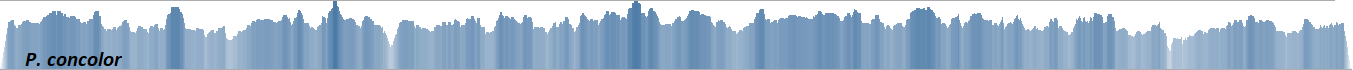
\includegraphics[width=\linewidth]{S1_A}
		\caption{\textit{P.concolor}}\label{fig:s1a}		
	\end{subfigure}
		\begin{subfigure}[t]{\linewidth}
		\centering
		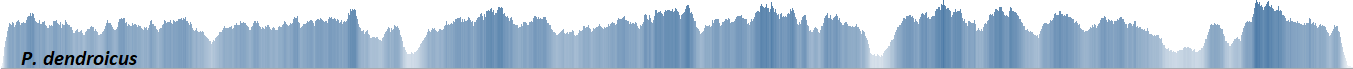
\includegraphics[width=\linewidth]{S1_B}
		\caption{}
	\end{subfigure}
	\begin{subfigure}[t]{\linewidth}
		\centering
		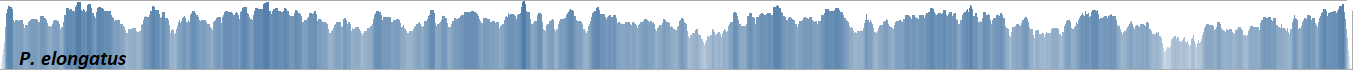
\includegraphics[width=\linewidth]{S1_C}
		\caption{}
	\end{subfigure}
	\begin{subfigure}[t]{\linewidth}
		\centering
		
\includegraphics[width=\linewidth]{S1_D}
		\caption{}		
	\end{subfigure}
	\begin{subfigure}[t]{\linewidth}
		\centering
		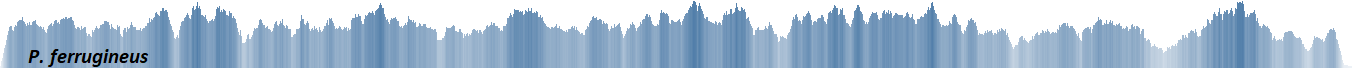
\includegraphics[width=\linewidth]{S1_E}
		\caption{}
	\end{subfigure}
	\begin{subfigure}[t]{\linewidth}
		\centering
		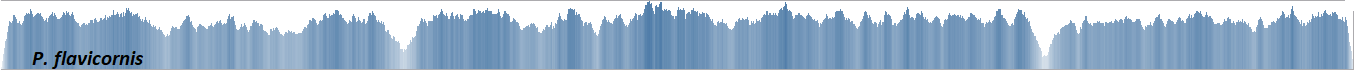
\includegraphics[width=\linewidth]{S1_F}
		\caption{}
	\end{subfigure}
	\begin{subfigure}[t]{\linewidth}
		\centering
		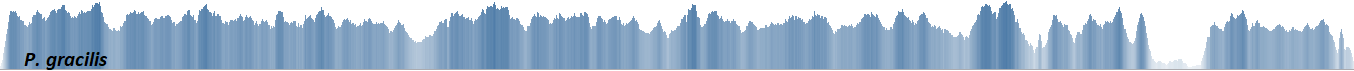
\includegraphics[width=\linewidth]{S1_G}
		\caption{}
	\end{subfigure}
	\begin{subfigure}[t]{\linewidth}
		\centering
		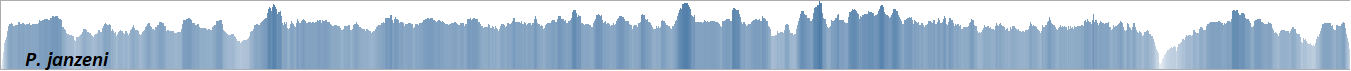
\includegraphics[width=\linewidth]{S1_H}
		\caption{}
	\end{subfigure}
\end{figure}

\begin{figure}\ContinuedFloat
	\begin{subfigure}[t]{\linewidth}
		\centering
		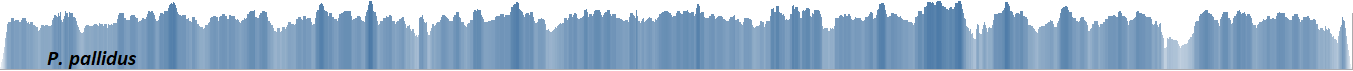
\includegraphics[width=\linewidth]{S1_I}
		\caption{}
	\end{subfigure}
	\begin{subfigure}[t]{\linewidth}
		\centering
		
\includegraphics[width=\linewidth]{S1_J}
		\caption{}
	\end{subfigure}
	\begin{subfigure}[t]{\linewidth}
		\centering
		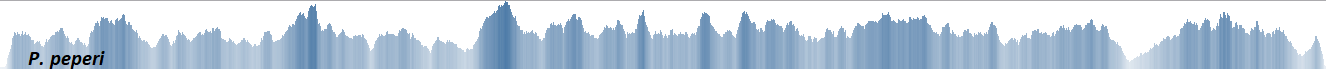
\includegraphics[width=\linewidth]{S1_K}
		\caption{}
	\end{subfigure}	
	\begin{subfigure}[t]{\linewidth}
		\centering
		
\includegraphics[width=\linewidth]{S1_L}
		\caption{}		
	\end{subfigure}
	\begin{subfigure}[t]{\linewidth}
		\centering
		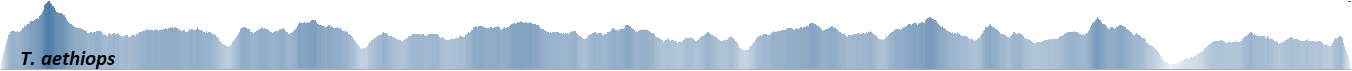
\includegraphics[width=\linewidth]{S1_M}
		\caption{}
	\end{subfigure}
	\begin{subfigure}[t]{\linewidth}
		\centering
		
\includegraphics[width=\linewidth]{S1_N}
		\caption{}
	\end{subfigure}
\end{figure}	
	
	\newpage
	
	\newgeometry{left=.5cm, right=.5cm}
	\centering
	\begin{longtable}{llllllllllllllllllllll}
		\caption{Anotação completa dos 14 genomas mitocondriais descritos nessa dissertação}\label{tab:s1}\\
			1            & \multicolumn{2}{l}{}        & \multicolumn{2}{l}{}        & \multicolumn{2}{l}{}            & \multicolumn{3}{l}{Pseudomyrmex 				gracilis} & \multicolumn{3}{l}{}      & \multicolumn{3}{l}{}        & \multicolumn{3}{l}{}            & \multicolumn{3}{l}{}         \\
			Gene         & \multicolumn{4}{l}{Position}                              & \multicolumn{5}{l}{Size}                                                        & \multicolumn{6}{l}{Codon}                               & \multicolumn{3}{l}{Intergenic}  & \multicolumn{3}{l}{}         \\
			& \multicolumn{2}{l}{From}    & \multicolumn{2}{l}{To}      & \multicolumn{2}{l}{Nucleotide}  & \multicolumn{3}{l}{Aminoacid}                 & \multicolumn{3}{l}{Start} & \multicolumn{3}{l}{Stop}    & \multicolumn{3}{l}{nucleotide}  & \multicolumn{3}{l}{}         \\
			COX1         & \multicolumn{2}{l}{1}       & \multicolumn{2}{l}{1533}    & \multicolumn{2}{l}{1533}        & \multicolumn{3}{l}{510}                       & \multicolumn{3}{l}{ATG}   & \multicolumn{3}{l}{TAA}     & \multicolumn{3}{l}{0}           & \multicolumn{3}{l}{}         \\
			tRNA(Leu)    & \multicolumn{2}{l}{1534}    & \multicolumn{2}{l}{1599}    & \multicolumn{2}{l}{66}          & \multicolumn{3}{l}{}                          & \multicolumn{3}{l}{}      & \multicolumn{3}{l}{}        & \multicolumn{3}{l}{0}           & \multicolumn{3}{l}{}         \\
			COX2         & \multicolumn{2}{l}{1600}    & \multicolumn{2}{l}{2271}    & \multicolumn{2}{l}{672}         & \multicolumn{3}{l}{223}                       & \multicolumn{3}{l}{ATC}   & \multicolumn{3}{l}{TAA}     & \multicolumn{3}{l}{16}          & \multicolumn{3}{l}{}         \\
			tRNA(Lys)    & \multicolumn{2}{l}{2288}    & \multicolumn{2}{l}{2359}    & \multicolumn{2}{l}{72}          & \multicolumn{3}{l}{}                          & \multicolumn{3}{l}{}      & \multicolumn{3}{l}{}        & \multicolumn{3}{l}{0}           & \multicolumn{3}{l}{}         \\
			tRNA(Asp)    & \multicolumn{2}{l}{2360}    & \multicolumn{2}{l}{2422}    & \multicolumn{2}{l}{63}          & \multicolumn{3}{l}{}                          & \multicolumn{3}{l}{}      & \multicolumn{3}{l}{}        & \multicolumn{3}{l}{0}           & \multicolumn{3}{l}{}         \\
			ATP8         & \multicolumn{2}{l}{2423}    & \multicolumn{2}{l}{2584}    & \multicolumn{2}{l}{162}         & \multicolumn{3}{l}{53}                        & \multicolumn{3}{l}{ATT}   & \multicolumn{3}{l}{TAA}     & \multicolumn{3}{l}{21}          & \multicolumn{3}{l}{}         \\
			ATP6         & \multicolumn{2}{l}{2606}    & \multicolumn{2}{l}{3272}    & \multicolumn{2}{l}{667}         & \multicolumn{3}{l}{222}                       & \multicolumn{3}{l}{ATG}   & \multicolumn{3}{l}{T-}      & \multicolumn{3}{l}{0}           & \multicolumn{3}{l}{}         \\
			COX3         & \multicolumn{2}{l}{3273}    & \multicolumn{2}{l}{4052}    & \multicolumn{2}{l}{780}         & \multicolumn{3}{l}{259}                       & \multicolumn{3}{l}{ATG}   & \multicolumn{3}{l}{TAA}     & \multicolumn{3}{l}{3}           & \multicolumn{3}{l}{}         \\
			tRNA(Gly)    & \multicolumn{2}{l}{4056}    & \multicolumn{2}{l}{4125}    & \multicolumn{2}{l}{70}          & \multicolumn{3}{l}{}                          & \multicolumn{3}{l}{}      & \multicolumn{3}{l}{}        & \multicolumn{3}{l}{3}           & \multicolumn{3}{l}{}         \\
			ND3          & \multicolumn{2}{l}{4129}    & \multicolumn{2}{l}{4479}    & \multicolumn{2}{l}{351}         & \multicolumn{3}{l}{116}                       & \multicolumn{3}{l}{ATG}   & \multicolumn{3}{l}{TAA}     & \multicolumn{3}{l}{6}           & \multicolumn{3}{l}{}         \\
			tRNA(Ala)    & \multicolumn{2}{l}{4486}    & \multicolumn{2}{l}{4547}    & \multicolumn{2}{l}{62}          & \multicolumn{3}{l}{}                          & \multicolumn{3}{l}{}      & \multicolumn{3}{l}{}        & \multicolumn{3}{l}{0}           & \multicolumn{3}{l}{}         \\
			tRNA(Arg)    & \multicolumn{2}{l}{4548}    & \multicolumn{2}{l}{4615}    & \multicolumn{2}{l}{68}          & \multicolumn{3}{l}{}                          & \multicolumn{3}{l}{}      & \multicolumn{3}{l}{}        & \multicolumn{3}{l}{2}           & \multicolumn{3}{l}{}         \\
			tRNA(Asn)    & \multicolumn{2}{l}{4618}    & \multicolumn{2}{l}{4684}    & \multicolumn{2}{l}{67}          & \multicolumn{3}{l}{}                          & \multicolumn{3}{l}{}      & \multicolumn{3}{l}{}        & \multicolumn{3}{l}{28}          & \multicolumn{3}{l}{}         \\
			tRNA(Ser)    & \multicolumn{2}{l}{4713}    & \multicolumn{2}{l}{4772}    & \multicolumn{2}{l}{60}          & \multicolumn{3}{l}{}                          & \multicolumn{3}{l}{}      & \multicolumn{3}{l}{}        & \multicolumn{3}{l}{5}           & \multicolumn{3}{l}{}         \\
			tRNA(Glu)    & \multicolumn{2}{l}{4778}    & \multicolumn{2}{l}{4850}    & \multicolumn{2}{l}{73}          & \multicolumn{3}{l}{}                          & \multicolumn{3}{l}{}      & \multicolumn{3}{l}{}        & \multicolumn{3}{l}{10}          & \multicolumn{3}{l}{}         \\
			tRNA(Phe)    & \multicolumn{2}{l}{4861}    & \multicolumn{2}{l}{4929}    & \multicolumn{2}{l}{69}          & \multicolumn{3}{l}{}                          & \multicolumn{3}{l}{}      & \multicolumn{3}{l}{}        & \multicolumn{3}{l}{39}          & \multicolumn{3}{l}{}         \\
			ND5          & \multicolumn{2}{l}{4969}    & \multicolumn{2}{l}{6633}    & \multicolumn{2}{l}{1665}        & \multicolumn{3}{l}{554}                       & \multicolumn{3}{l}{ATT}   & \multicolumn{3}{l}{TAA}     & \multicolumn{3}{l}{0}           & \multicolumn{3}{l}{}         \\
			tRNA(His)    & \multicolumn{2}{l}{6634}    & \multicolumn{2}{l}{6698}    & \multicolumn{2}{l}{65}          & \multicolumn{3}{l}{}                          & \multicolumn{3}{l}{}      & \multicolumn{3}{l}{}        & \multicolumn{3}{l}{0}           & \multicolumn{3}{l}{}         \\
			ND4          & \multicolumn{2}{l}{6699}    & \multicolumn{2}{l}{8022}    & \multicolumn{2}{l}{1324}        & \multicolumn{3}{l}{441}                       & \multicolumn{3}{l}{ATG}   & \multicolumn{3}{l}{T-}      & \multicolumn{3}{l}{0}           & \multicolumn{3}{l}{}         \\
			ND4L         & \multicolumn{2}{l}{8023}    & \multicolumn{2}{l}{8305}    & \multicolumn{2}{l}{283}         & \multicolumn{3}{l}{94}                        & \multicolumn{3}{l}{ATA}   & \multicolumn{3}{l}{T-}      & \multicolumn{3}{l}{27}          & \multicolumn{3}{l}{}         \\
			tRNA(Thr)    & \multicolumn{2}{l}{8333}    & \multicolumn{2}{l}{8398}    & \multicolumn{2}{l}{66}          & \multicolumn{3}{l}{}                          & \multicolumn{3}{l}{}      & \multicolumn{3}{l}{}        & \multicolumn{3}{l}{1}           & \multicolumn{3}{l}{}         \\
			tRNA(Pro)    & \multicolumn{2}{l}{8400}    & \multicolumn{2}{l}{8466}    & \multicolumn{2}{l}{67}          & \multicolumn{3}{l}{}                          & \multicolumn{3}{l}{}      & \multicolumn{3}{l}{}        & \multicolumn{3}{l}{20}          & \multicolumn{3}{l}{}         \\
			ND6          & \multicolumn{2}{l}{8487}    & \multicolumn{2}{l}{9018}    & \multicolumn{2}{l}{532}         & \multicolumn{3}{l}{177}                       & \multicolumn{3}{l}{ATG}   & \multicolumn{3}{l}{T-}      & \multicolumn{3}{l}{0}           & \multicolumn{3}{l}{}         \\
			CYTB         & \multicolumn{2}{l}{9019}    & \multicolumn{2}{l}{10139}   & \multicolumn{2}{l}{1120}        & \multicolumn{3}{l}{373}                       & \multicolumn{3}{l}{ATG}   & \multicolumn{3}{l}{TA-}     & \multicolumn{3}{l}{0}           & \multicolumn{3}{l}{}         \\
			tRNA(Ser)    & \multicolumn{2}{l}{10140}   & \multicolumn{2}{l}{10208}   & \multicolumn{2}{l}{69}          & \multicolumn{3}{l}{}                          & \multicolumn{3}{l}{}      & \multicolumn{3}{l}{}        & \multicolumn{3}{l}{11}          & \multicolumn{3}{l}{}         \\
			ND1          & \multicolumn{2}{l}{10220}   & \multicolumn{2}{l}{11170}   & \multicolumn{2}{l}{951}         & \multicolumn{3}{l}{316}                       & \multicolumn{3}{l}{ATT}   & \multicolumn{3}{l}{TAA}     & \multicolumn{3}{l}{0}           & \multicolumn{3}{l}{}         \\
			tRNA(Leu)    & \multicolumn{2}{l}{11171}   & \multicolumn{2}{l}{11238}   & \multicolumn{2}{l}{68}          & \multicolumn{3}{l}{}                          & \multicolumn{3}{l}{}      & \multicolumn{3}{l}{}        & \multicolumn{3}{l}{11}          & \multicolumn{3}{l}{}         \\
			16S 				rRNA & \multicolumn{2}{l}{11250}   & \multicolumn{2}{l}{12527}   & \multicolumn{2}{l}{1278}        & \multicolumn{3}{l}{}                          & \multicolumn{3}{l}{}      & \multicolumn{3}{l}{}        & \multicolumn{3}{l}{20}          & \multicolumn{3}{l}{}         \\
			tRNA(Val)    & \multicolumn{2}{l}{12548}   & \multicolumn{2}{l}{12615}   & \multicolumn{2}{l}{68}          & \multicolumn{3}{l}{}                          & \multicolumn{3}{l}{}      & \multicolumn{3}{l}{}        & \multicolumn{3}{l}{10}          & \multicolumn{3}{l}{}         \\
			12S 				rRNA & \multicolumn{2}{l}{12626}   & \multicolumn{2}{l}{13401}   & \multicolumn{2}{l}{776}         & \multicolumn{3}{l}{}                          & \multicolumn{3}{l}{}      & \multicolumn{3}{l}{}        & \multicolumn{3}{l}{628}         & \multicolumn{3}{l}{}         \\
			tRNA(Met)    & \multicolumn{2}{l}{14030}   & \multicolumn{2}{l}{14098}   & \multicolumn{2}{l}{69}          & \multicolumn{3}{l}{}                          & \multicolumn{3}{l}{}      & \multicolumn{3}{l}{}        & \multicolumn{3}{l}{0}           & \multicolumn{3}{l}{}         \\
			tRNA(Ile)    & \multicolumn{2}{l}{14099}   & \multicolumn{2}{l}{14165}   & \multicolumn{2}{l}{67}          & \multicolumn{3}{l}{}                          & \multicolumn{3}{l}{}      & \multicolumn{3}{l}{}        & \multicolumn{3}{l}{45}          & \multicolumn{3}{l}{}         \\
			tRNA(Gln)    & \multicolumn{2}{l}{14211}   & \multicolumn{2}{l}{14280}   & \multicolumn{2}{l}{70}          & \multicolumn{3}{l}{}                          & \multicolumn{3}{l}{}      & \multicolumn{3}{l}{}        & \multicolumn{3}{l}{61}          & \multicolumn{3}{l}{}         \\
			ND2          & \multicolumn{2}{l}{14342}   & \multicolumn{2}{l}{15303}   & \multicolumn{2}{l}{961}         & \multicolumn{3}{l}{320}                       & \multicolumn{3}{l}{ATT}   & \multicolumn{3}{l}{TA-}     & \multicolumn{3}{l}{0}           & \multicolumn{3}{l}{}         \\
			tRNA(Trp)    & \multicolumn{2}{l}{15304}   & \multicolumn{2}{l}{15369}   & \multicolumn{2}{l}{66}          & \multicolumn{3}{l}{}                          & \multicolumn{3}{l}{}      & \multicolumn{3}{l}{}        & \multicolumn{3}{l}{1}           & \multicolumn{3}{l}{}         \\
			tRNA(Cys)    & \multicolumn{2}{l}{15371}   & \multicolumn{2}{l}{15434}   & \multicolumn{2}{l}{64}          & \multicolumn{3}{l}{}                          & \multicolumn{3}{l}{}      & \multicolumn{3}{l}{}        & \multicolumn{3}{l}{38}          & \multicolumn{3}{l}{}         \\
			tRNA(Tyr)    & \multicolumn{2}{l}{15473}   & \multicolumn{2}{l}{15538}   & \multicolumn{2}{l}{66}          & \multicolumn{3}{l}{}                          & \multicolumn{3}{l}{}      & \multicolumn{3}{l}{}        & \multicolumn{3}{l}{166}         & \multicolumn{3}{l}{}         \\
			2            & \multicolumn{2}{l}{}        & \multicolumn{2}{l}{}        & \multicolumn{8}{l}{\begin{tabular}[c]{@{}l@{}}Pseudomyrmex\\   				concolor\end{tabular}}                   & \multicolumn{3}{l}{}        & \multicolumn{3}{l}{}            & \multicolumn{3}{l}{}         \\
			Gene         & \multicolumn{4}{l}{Position}                              & \multicolumn{5}{l}{Size}                                                        & \multicolumn{6}{l}{Codon}                               & \multicolumn{3}{l}{Intergenic}  & \multicolumn{3}{l}{}         \\
			& \multicolumn{2}{l}{From}    & \multicolumn{2}{l}{To}      & \multicolumn{2}{l}{Nucleotide}  & \multicolumn{3}{l}{Aminoacid}                 & \multicolumn{3}{l}{Start} & \multicolumn{3}{l}{Stop}    & \multicolumn{3}{l}{nucleotide}  & \multicolumn{3}{l}{}         \\
			COX1         & \multicolumn{2}{l}{1}       & \multicolumn{2}{l}{1533}    & \multicolumn{2}{l}{1533}        & \multicolumn{3}{l}{510}                       & \multicolumn{3}{l}{ATG}   & \multicolumn{3}{l}{TAA}     & \multicolumn{3}{l}{2}           & \multicolumn{3}{l}{}         \\
			tRNA(Leu)    & \multicolumn{2}{l}{1536}    & \multicolumn{2}{l}{1607}    & \multicolumn{2}{l}{72}          & \multicolumn{3}{l}{}                          & \multicolumn{3}{l}{}      & \multicolumn{3}{l}{}        & \multicolumn{3}{l}{0}           & \multicolumn{3}{l}{}         \\
			COX2         & \multicolumn{2}{l}{1608}    & \multicolumn{2}{l}{2285}    & \multicolumn{2}{l}{678}         & \multicolumn{3}{l}{225}                       & \multicolumn{3}{l}{ATA}   & \multicolumn{3}{l}{TAA}     & \multicolumn{3}{l}{60}          & \multicolumn{3}{l}{}         \\
			tRNA(Lys)    & \multicolumn{2}{l}{2346}    & \multicolumn{2}{l}{2415}    & \multicolumn{2}{l}{70}          & \multicolumn{3}{l}{}                          & \multicolumn{3}{l}{}      & \multicolumn{3}{l}{}        & \multicolumn{3}{l}{0}           & \multicolumn{3}{l}{}         \\
			tRNA(Asp)    & \multicolumn{2}{l}{2416}    & \multicolumn{2}{l}{2482}    & \multicolumn{2}{l}{67}          & \multicolumn{3}{l}{}                          & \multicolumn{3}{l}{}      & \multicolumn{3}{l}{}        & \multicolumn{3}{l}{0}           & \multicolumn{3}{l}{}         \\
			ATP8         & \multicolumn{2}{l}{2483}    & \multicolumn{2}{l}{2662}    & \multicolumn{2}{l}{180}         & \multicolumn{3}{l}{59}                        & \multicolumn{3}{l}{ATT}   & \multicolumn{3}{l}{TAA}     & \multicolumn{3}{l}{35}          & \multicolumn{3}{l}{}         \\
			ATP6         & \multicolumn{2}{l}{2698}    & \multicolumn{2}{l}{3361}    & \multicolumn{2}{l}{664}         & \multicolumn{3}{l}{221}                       & \multicolumn{3}{l}{ATG}   & \multicolumn{3}{l}{T-}      & \multicolumn{3}{l}{0}           & \multicolumn{3}{l}{}         \\
			COX3         & \multicolumn{2}{l}{3362}    & \multicolumn{2}{l}{4141}    & \multicolumn{2}{l}{780}         & \multicolumn{3}{l}{259}                       & \multicolumn{3}{l}{ATG}   & \multicolumn{3}{l}{TAA}     & \multicolumn{3}{l}{26}          & \multicolumn{3}{l}{}         \\
			tRNA(Gly)    & \multicolumn{2}{l}{4168}    & \multicolumn{2}{l}{4245}    & \multicolumn{2}{l}{78}          & \multicolumn{3}{l}{}                          & \multicolumn{3}{l}{}      & \multicolumn{3}{l}{}        & \multicolumn{3}{l}{4}           & \multicolumn{3}{l}{}         \\
			ND3          & \multicolumn{2}{l}{4250}    & \multicolumn{2}{l}{4597}    & \multicolumn{2}{l}{348}         & \multicolumn{3}{l}{115}                       & \multicolumn{3}{l}{ATG}   & \multicolumn{3}{l}{TAA}     & \multicolumn{3}{l}{71}          & \multicolumn{3}{l}{}         \\
			tRNA(Ala)    & \multicolumn{2}{l}{4669}    & \multicolumn{2}{l}{4737}    & \multicolumn{2}{l}{69}          & \multicolumn{3}{l}{}                          & \multicolumn{3}{l}{}      & \multicolumn{3}{l}{}        & \multicolumn{3}{l}{0}           & \multicolumn{3}{l}{}         \\
			tRNA(Arg)    & \multicolumn{2}{l}{4738}    & \multicolumn{2}{l}{4805}    & \multicolumn{2}{l}{68}          & \multicolumn{3}{l}{}                          & \multicolumn{3}{l}{}      & \multicolumn{3}{l}{}        & \multicolumn{3}{l}{7}           & \multicolumn{3}{l}{}         \\
			tRNA(Asn)    & \multicolumn{2}{l}{4813}    & \multicolumn{2}{l}{4879}    & \multicolumn{2}{l}{67}          & \multicolumn{3}{l}{}                          & \multicolumn{3}{l}{}      & \multicolumn{3}{l}{}        & \multicolumn{3}{l}{15}          & \multicolumn{3}{l}{}         \\
			tRNA(Ser)    & \multicolumn{2}{l}{4895}    & \multicolumn{2}{l}{4952}    & \multicolumn{2}{l}{58}          & \multicolumn{3}{l}{}                          & \multicolumn{3}{l}{}      & \multicolumn{3}{l}{}        & \multicolumn{3}{l}{19}          & \multicolumn{3}{l}{}         \\
			tRNA(Glu)    & \multicolumn{2}{l}{4972}    & \multicolumn{2}{l}{5044}    & \multicolumn{2}{l}{73}          & \multicolumn{3}{l}{}                          & \multicolumn{3}{l}{}      & \multicolumn{3}{l}{}        & \multicolumn{3}{l}{106}         & \multicolumn{3}{l}{}         \\
			tRNA(Phe)    & \multicolumn{2}{l}{5151}    & \multicolumn{2}{l}{5220}    & \multicolumn{2}{l}{70}          & \multicolumn{3}{l}{}                          & \multicolumn{3}{l}{}      & \multicolumn{3}{l}{}        & \multicolumn{3}{l}{3}           & \multicolumn{3}{l}{}         \\
			ND5          & \multicolumn{2}{l}{5224}    & \multicolumn{2}{l}{6885}    & \multicolumn{2}{l}{1662}        & \multicolumn{3}{l}{553}                       & \multicolumn{3}{l}{GTG}   & \multicolumn{3}{l}{TAA}     & \multicolumn{3}{l}{0}           & \multicolumn{3}{l}{}         \\
			tRNA(His)    & \multicolumn{2}{l}{6886}    & \multicolumn{2}{l}{6954}    & \multicolumn{2}{l}{69}          & \multicolumn{3}{l}{}                          & \multicolumn{3}{l}{}      & \multicolumn{3}{l}{}        & \multicolumn{3}{l}{6}           & \multicolumn{3}{l}{}         \\
			ND4          & \multicolumn{2}{l}{6961}    & \multicolumn{2}{l}{8283}    & \multicolumn{2}{l}{1323}        & \multicolumn{3}{l}{440}                       & \multicolumn{3}{l}{ATG}   & \multicolumn{3}{l}{TAA}     & \multicolumn{3}{l}{0}           & \multicolumn{3}{l}{}         \\
			ND4L         & \multicolumn{2}{l}{8284}    & \multicolumn{2}{l}{8566}    & \multicolumn{2}{l}{283}         & \multicolumn{3}{l}{94}                        & \multicolumn{3}{l}{ATA}   & \multicolumn{3}{l}{T-}      & \multicolumn{3}{l}{97}          & \multicolumn{3}{l}{}         \\
			tRNA(Thr)    & \multicolumn{2}{l}{8664}    & \multicolumn{2}{l}{8730}    & \multicolumn{2}{l}{67}          & \multicolumn{3}{l}{}                          & \multicolumn{3}{l}{}      & \multicolumn{3}{l}{}        & \multicolumn{3}{l}{26}          & \multicolumn{3}{l}{}         \\
			tRNA(Pro)    & \multicolumn{2}{l}{8757}    & \multicolumn{2}{l}{8823}    & \multicolumn{2}{l}{67}          & \multicolumn{3}{l}{}                          & \multicolumn{3}{l}{}      & \multicolumn{3}{l}{}        & \multicolumn{3}{l}{17}          & \multicolumn{3}{l}{}         \\
			ND6          & \multicolumn{2}{l}{8841}    & \multicolumn{2}{l}{9372}    & \multicolumn{2}{l}{532}         & \multicolumn{3}{l}{177}                       & \multicolumn{3}{l}{ATG}   & \multicolumn{3}{l}{T-}      & \multicolumn{3}{l}{0}           & \multicolumn{3}{l}{}         \\
			CYTB         & \multicolumn{2}{l}{9373}    & \multicolumn{2}{l}{10493}   & \multicolumn{2}{l}{1121}        & \multicolumn{3}{l}{373}                       & \multicolumn{3}{l}{ATG}   & \multicolumn{3}{l}{TA-}     & \multicolumn{3}{l}{0}           & \multicolumn{3}{l}{}         \\
			tRNA(Ser)    & \multicolumn{2}{l}{10494}   & \multicolumn{2}{l}{10563}   & \multicolumn{2}{l}{70}          & \multicolumn{3}{l}{}                          & \multicolumn{3}{l}{}      & \multicolumn{3}{l}{}        & \multicolumn{3}{l}{3}           & \multicolumn{3}{l}{}         \\
			ND1          & \multicolumn{2}{l}{10567}   & \multicolumn{2}{l}{11514}   & \multicolumn{2}{l}{948}         & \multicolumn{3}{l}{315}                       & \multicolumn{3}{l}{ATT}   & \multicolumn{3}{l}{TAG}     & \multicolumn{3}{l}{0}           & \multicolumn{3}{l}{}         \\
			tRNA(Leu)    & \multicolumn{2}{l}{11515}   & \multicolumn{2}{l}{11582}   & \multicolumn{2}{l}{68}          & \multicolumn{3}{l}{}                          & \multicolumn{3}{l}{}      & \multicolumn{3}{l}{}        & \multicolumn{3}{l}{7}           & \multicolumn{3}{l}{}         \\
			16S 				rRNA & \multicolumn{2}{l}{11590}   & \multicolumn{2}{l}{12880}   & \multicolumn{2}{l}{1291}        & \multicolumn{3}{l}{}                          & \multicolumn{3}{l}{}      & \multicolumn{3}{l}{}        & \multicolumn{3}{l}{0}           & \multicolumn{3}{l}{}         \\
			tRNA(Val)    & \multicolumn{2}{l}{12881}   & \multicolumn{2}{l}{12971}   & \multicolumn{2}{l}{91}          & \multicolumn{3}{l}{}                          & \multicolumn{3}{l}{}      & \multicolumn{3}{l}{}        & \multicolumn{3}{l}{2}           & \multicolumn{3}{l}{}         \\
			12S 				rRNA & \multicolumn{2}{l}{12974}   & \multicolumn{2}{l}{13760}   & \multicolumn{2}{l}{787}         & \multicolumn{3}{l}{}                          & \multicolumn{3}{l}{}      & \multicolumn{3}{l}{}        & \multicolumn{3}{l}{527}         & \multicolumn{3}{l}{}         \\
			tRNA(Met)    & \multicolumn{2}{l}{14288}   & \multicolumn{2}{l}{14357}   & \multicolumn{2}{l}{70}          & \multicolumn{3}{l}{}                          & \multicolumn{3}{l}{}      & \multicolumn{3}{l}{}        & \multicolumn{3}{l}{5}           & \multicolumn{3}{l}{}         \\
			tRNA(Ile)    & \multicolumn{2}{l}{14363}   & \multicolumn{2}{l}{14431}   & \multicolumn{2}{l}{69}          & \multicolumn{3}{l}{}                          & \multicolumn{3}{l}{}      & \multicolumn{3}{l}{}        & \multicolumn{3}{l}{40}          & \multicolumn{3}{l}{}         \\
			tRNA(Gln)    & \multicolumn{2}{l}{14472}   & \multicolumn{2}{l}{14546}   & \multicolumn{2}{l}{75}          & \multicolumn{3}{l}{}                          & \multicolumn{3}{l}{}      & \multicolumn{3}{l}{}        & \multicolumn{3}{l}{56}          & \multicolumn{3}{l}{}         \\
			ND2          & \multicolumn{2}{l}{14603}   & \multicolumn{2}{l}{15571}   & \multicolumn{2}{l}{969}         & \multicolumn{3}{l}{322}                       & \multicolumn{3}{l}{ATA}   & \multicolumn{3}{l}{TAA}     & \multicolumn{3}{l}{8}           & \multicolumn{3}{l}{}         \\
			tRNA(Trp)    & \multicolumn{2}{l}{15580}   & \multicolumn{2}{l}{15650}   & \multicolumn{2}{l}{71}          & \multicolumn{3}{l}{}                          & \multicolumn{3}{l}{}      & \multicolumn{3}{l}{}        & \multicolumn{3}{l}{20}          & \multicolumn{3}{l}{}         \\
			tRNA(Cys)    & \multicolumn{2}{l}{15671}   & \multicolumn{2}{l}{15733}   & \multicolumn{2}{l}{63}          & \multicolumn{3}{l}{}                          & \multicolumn{3}{l}{}      & \multicolumn{3}{l}{}        & \multicolumn{3}{l}{48}          & \multicolumn{3}{l}{}         \\
			tRNA(Tyr)    & \multicolumn{2}{l}{15782}   & \multicolumn{2}{l}{15850}   & \multicolumn{2}{l}{69}          & \multicolumn{3}{l}{}                          & \multicolumn{3}{l}{}      & \multicolumn{3}{l}{}        & \multicolumn{3}{l}{56}          & \multicolumn{3}{l}{}         \\
			3            & \multicolumn{2}{l}{}        & \multicolumn{2}{l}{}        & \multicolumn{8}{l}{\begin{tabular}[c]{@{}l@{}}Pseudomyrmex\\   				elongatus\end{tabular}}                  & \multicolumn{3}{l}{}        & \multicolumn{3}{l}{}            & \multicolumn{3}{l}{}         \\
			Gene         & \multicolumn{4}{l}{Position}                              & \multicolumn{5}{l}{Size}                                                        & \multicolumn{6}{l}{Codon}                               & \multicolumn{3}{l}{Intergenic}  & \multicolumn{3}{l}{}         \\
			& \multicolumn{2}{l}{From}    & \multicolumn{2}{l}{To}      & \multicolumn{2}{l}{Nucleotide}  & \multicolumn{3}{l}{Aminoacid}                 & \multicolumn{3}{l}{Start} & \multicolumn{3}{l}{Stop}    & \multicolumn{3}{l}{nucleotide}  & \multicolumn{3}{l}{}         \\
			COX1         & \multicolumn{2}{l}{1}       & \multicolumn{2}{l}{1531}    & \multicolumn{2}{l}{1531}        & \multicolumn{3}{l}{510}                       & \multicolumn{3}{l}{ATG}   & \multicolumn{3}{l}{T-}      & \multicolumn{3}{l}{0}           & \multicolumn{3}{l}{}         \\
			tRNA(Leu)    & \multicolumn{2}{l}{1532}    & \multicolumn{2}{l}{1599}    & \multicolumn{2}{l}{68}          & \multicolumn{3}{l}{}                          & \multicolumn{3}{l}{}      & \multicolumn{3}{l}{}        & \multicolumn{3}{l}{0}           & \multicolumn{3}{l}{}         \\
			COX2         & \multicolumn{2}{l}{1600}    & \multicolumn{2}{l}{2277}    & \multicolumn{2}{l}{678}         & \multicolumn{3}{l}{225}                       & \multicolumn{3}{l}{ATT}   & \multicolumn{3}{l}{TAA}     & \multicolumn{3}{l}{94}          & \multicolumn{3}{l}{}         \\
			tRNA(Lys)    & \multicolumn{2}{l}{2372}    & \multicolumn{2}{l}{2444}    & \multicolumn{2}{l}{73}          & \multicolumn{3}{l}{}                          & \multicolumn{3}{l}{}      & \multicolumn{3}{l}{}        & \multicolumn{3}{l}{0}           & \multicolumn{3}{l}{}         \\
			tRNA(Asp)    & \multicolumn{2}{l}{2445}    & \multicolumn{2}{l}{2513}    & \multicolumn{2}{l}{69}          & \multicolumn{3}{l}{}                          & \multicolumn{3}{l}{}      & \multicolumn{3}{l}{}        & \multicolumn{3}{l}{0}           & \multicolumn{3}{l}{}         \\
			ATP8         & \multicolumn{2}{l}{2514}    & \multicolumn{2}{l}{2690}    & \multicolumn{2}{l}{177}         & \multicolumn{3}{l}{58}                        & \multicolumn{3}{l}{ATT}   & \multicolumn{3}{l}{TAA}     & \multicolumn{3}{l}{165}         & \multicolumn{3}{l}{}         \\
			ATP6         & \multicolumn{2}{l}{2856}    & \multicolumn{2}{l}{3522}    & \multicolumn{2}{l}{667}         & \multicolumn{3}{l}{222}                       & \multicolumn{3}{l}{ATG}   & \multicolumn{3}{l}{T-}      & \multicolumn{3}{l}{0}           & \multicolumn{3}{l}{}         \\
			COX3         & \multicolumn{2}{l}{3523}    & \multicolumn{2}{l}{4302}    & \multicolumn{2}{l}{780}         & \multicolumn{3}{l}{259}                       & \multicolumn{3}{l}{ATG}   & \multicolumn{3}{l}{TAA}     & \multicolumn{3}{l}{15}          & \multicolumn{3}{l}{}         \\
			tRNA(Gly)    & \multicolumn{2}{l}{4318}    & \multicolumn{2}{l}{4385}    & \multicolumn{2}{l}{68}          & \multicolumn{3}{l}{}                          & \multicolumn{3}{l}{}      & \multicolumn{3}{l}{}        & \multicolumn{3}{l}{5}           & \multicolumn{3}{l}{}         \\
			ND3          & \multicolumn{2}{l}{4391}    & \multicolumn{2}{l}{4738}    & \multicolumn{2}{l}{348}         & \multicolumn{3}{l}{115}                       & \multicolumn{3}{l}{ATG}   & \multicolumn{3}{l}{TAA}     & \multicolumn{3}{l}{62}          & \multicolumn{3}{l}{}         \\
			tRNA(Ala)    & \multicolumn{2}{l}{4801}    & \multicolumn{2}{l}{4869}    & \multicolumn{2}{l}{69}          & \multicolumn{3}{l}{}                          & \multicolumn{3}{l}{}      & \multicolumn{3}{l}{}        & \multicolumn{3}{l}{0}           & \multicolumn{3}{l}{}         \\
			tRNA(Arg)    & \multicolumn{2}{l}{4870}    & \multicolumn{2}{l}{4937}    & \multicolumn{2}{l}{68}          & \multicolumn{3}{l}{}                          & \multicolumn{3}{l}{}      & \multicolumn{3}{l}{}        & \multicolumn{3}{l}{0}           & \multicolumn{3}{l}{}         \\
			tRNA(Asn)    & \multicolumn{2}{l}{4938}    & \multicolumn{2}{l}{5008}    & \multicolumn{2}{l}{71}          & \multicolumn{3}{l}{}                          & \multicolumn{3}{l}{}      & \multicolumn{3}{l}{}        & \multicolumn{3}{l}{9}           & \multicolumn{3}{l}{}         \\
			tRNA(Ser)    & \multicolumn{2}{l}{5018}    & \multicolumn{2}{l}{5079}    & \multicolumn{2}{l}{62}          & \multicolumn{3}{l}{}                          & \multicolumn{3}{l}{}      & \multicolumn{3}{l}{}        & \multicolumn{3}{l}{35}          & \multicolumn{3}{l}{}         \\
			tRNA(Glu)    & \multicolumn{2}{l}{5115}    & \multicolumn{2}{l}{5184}    & \multicolumn{2}{l}{70}          & \multicolumn{3}{l}{}                          & \multicolumn{3}{l}{}      & \multicolumn{3}{l}{}        & \multicolumn{3}{l}{159}         & \multicolumn{3}{l}{}         \\
			tRNA(Phe)    & \multicolumn{2}{l}{5344}    & \multicolumn{2}{l}{5412}    & \multicolumn{2}{l}{69}          & \multicolumn{3}{l}{}                          & \multicolumn{3}{l}{}      & \multicolumn{3}{l}{}        & \multicolumn{3}{l}{12}          & \multicolumn{3}{l}{}         \\
			ND5          & \multicolumn{2}{l}{5425}    & \multicolumn{2}{l}{7092}    & \multicolumn{2}{l}{1668}        & \multicolumn{3}{l}{555}                       & \multicolumn{3}{l}{ATG}   & \multicolumn{3}{l}{TAG}     & \multicolumn{3}{l}{0}           & \multicolumn{3}{l}{}         \\
			tRNA(His)    & \multicolumn{2}{l}{7093}    & \multicolumn{2}{l}{7159}    & \multicolumn{2}{l}{67}          & \multicolumn{3}{l}{}                          & \multicolumn{3}{l}{}      & \multicolumn{3}{l}{}        & \multicolumn{3}{l}{12}          & \multicolumn{3}{l}{}         \\
			ND4          & \multicolumn{2}{l}{7172}    & \multicolumn{2}{l}{8503}    & \multicolumn{2}{l}{1332}        & \multicolumn{3}{l}{443}                       & \multicolumn{3}{l}{ATG}   & \multicolumn{3}{l}{TAA}     & \multicolumn{3}{l}{0}           & \multicolumn{3}{l}{}         \\
			ND4L         & \multicolumn{2}{l}{8504}    & \multicolumn{2}{l}{8786}    & \multicolumn{2}{l}{283}         & \multicolumn{3}{l}{94}                        & \multicolumn{3}{l}{ATA}   & \multicolumn{3}{l}{T-}      & \multicolumn{3}{l}{129}         & \multicolumn{3}{l}{}         \\
			tRNA(Thr)    & \multicolumn{2}{l}{8916}    & \multicolumn{2}{l}{8984}    & \multicolumn{2}{l}{69}          & \multicolumn{3}{l}{}                          & \multicolumn{3}{l}{}      & \multicolumn{3}{l}{}        & \multicolumn{3}{l}{131}         & \multicolumn{3}{l}{}         \\
			tRNA(Pro)    & \multicolumn{2}{l}{9116}    & \multicolumn{2}{l}{9180}    & \multicolumn{2}{l}{65}          & \multicolumn{3}{l}{}                          & \multicolumn{3}{l}{}      & \multicolumn{3}{l}{}        & \multicolumn{3}{l}{136}         & \multicolumn{3}{l}{}         \\
			ND6          & \multicolumn{2}{l}{9317}    & \multicolumn{2}{l}{9848}    & \multicolumn{2}{l}{532}         & \multicolumn{3}{l}{177}                       & \multicolumn{3}{l}{ATG}   & \multicolumn{3}{l}{T-}      & \multicolumn{3}{l}{0}           & \multicolumn{3}{l}{}         \\
			CYTB         & \multicolumn{2}{l}{9849}    & \multicolumn{2}{l}{10964}   & \multicolumn{2}{l}{1116}        & \multicolumn{3}{l}{371}                       & \multicolumn{3}{l}{ATG}   & \multicolumn{3}{l}{TAG}     & \multicolumn{3}{l}{14}          & \multicolumn{3}{l}{}         \\
			tRNA(Ser)    & \multicolumn{2}{l}{10979}   & \multicolumn{2}{l}{11050}   & \multicolumn{2}{l}{72}          & \multicolumn{3}{l}{}                          & \multicolumn{3}{l}{}      & \multicolumn{3}{l}{}        & \multicolumn{3}{l}{604}         & \multicolumn{3}{l}{}         \\
			ND1          & \multicolumn{2}{l}{11655}   & \multicolumn{2}{l}{12605}   & \multicolumn{2}{l}{951}         & \multicolumn{3}{l}{316}                       & \multicolumn{3}{l}{ATG}   & \multicolumn{3}{l}{TAA}     & \multicolumn{3}{l}{0}           & \multicolumn{3}{l}{}         \\
			tRNA(Leu)    & \multicolumn{2}{l}{12606}   & \multicolumn{2}{l}{12672}   & \multicolumn{2}{l}{67}          & \multicolumn{3}{l}{}                          & \multicolumn{3}{l}{}      & \multicolumn{3}{l}{}        & \multicolumn{3}{l}{9}           & \multicolumn{3}{l}{}         \\
			16S 				rRNA & \multicolumn{2}{l}{12682}   & \multicolumn{2}{l}{14008}   & \multicolumn{2}{l}{1327}        & \multicolumn{3}{l}{}                          & \multicolumn{3}{l}{}      & \multicolumn{3}{l}{}        & \multicolumn{3}{l}{34}          & \multicolumn{3}{l}{}         \\
			tRNA(Val)    & \multicolumn{2}{l}{14043}   & \multicolumn{2}{l}{14097}   & \multicolumn{2}{l}{55}          & \multicolumn{3}{l}{}                          & \multicolumn{3}{l}{}      & \multicolumn{3}{l}{}        & \multicolumn{3}{l}{23}          & \multicolumn{3}{l}{}         \\
			12S 				rRNA & \multicolumn{2}{l}{14121}   & \multicolumn{2}{l}{14906}   & \multicolumn{2}{l}{786}         & \multicolumn{3}{l}{}                          & \multicolumn{3}{l}{}      & \multicolumn{3}{l}{}        & \multicolumn{3}{l}{697}         & \multicolumn{3}{l}{}         \\
			tRNA(Met)    & \multicolumn{2}{l}{15604}   & \multicolumn{2}{l}{15673}   & \multicolumn{2}{l}{70}          & \multicolumn{3}{l}{}                          & \multicolumn{3}{l}{}      & \multicolumn{3}{l}{}        & \multicolumn{3}{l}{6}           & \multicolumn{3}{l}{}         \\
			tRNA(Ile)    & \multicolumn{2}{l}{15680}   & \multicolumn{2}{l}{15747}   & \multicolumn{2}{l}{68}          & \multicolumn{3}{l}{}                          & \multicolumn{3}{l}{}      & \multicolumn{3}{l}{}        & \multicolumn{3}{l}{37}          & \multicolumn{3}{l}{}         \\
			tRNA(Gln)    & \multicolumn{2}{l}{15785}   & \multicolumn{2}{l}{15854}   & \multicolumn{2}{l}{70}          & \multicolumn{3}{l}{}                          & \multicolumn{3}{l}{}      & \multicolumn{3}{l}{}        & \multicolumn{3}{l}{72}          & \multicolumn{3}{l}{}         \\
			ND2          & \multicolumn{2}{l}{15927}   & \multicolumn{2}{l}{16892}   & \multicolumn{2}{l}{966}         & \multicolumn{3}{l}{321}                       & \multicolumn{3}{l}{ATA}   & \multicolumn{3}{l}{TAA}     & \multicolumn{3}{l}{2}           & \multicolumn{3}{l}{}         \\
			tRNA(Trp)    & \multicolumn{2}{l}{16895}   & \multicolumn{2}{l}{16964}   & \multicolumn{2}{l}{70}          & \multicolumn{3}{l}{}                          & \multicolumn{3}{l}{}      & \multicolumn{3}{l}{}        & \multicolumn{3}{l}{40}          & \multicolumn{3}{l}{}         \\
			tRNA(Cys)    & \multicolumn{2}{l}{17005}   & \multicolumn{2}{l}{17075}   & \multicolumn{2}{l}{71}          & \multicolumn{3}{l}{}                          & \multicolumn{3}{l}{}      & \multicolumn{3}{l}{}        & \multicolumn{3}{l}{92}          & \multicolumn{3}{l}{}         \\
			tRNA(Tyr)    & \multicolumn{2}{l}{17168}   & \multicolumn{2}{l}{17236}   & \multicolumn{2}{l}{69}          & \multicolumn{3}{l}{}                          & \multicolumn{3}{l}{}      & \multicolumn{3}{l}{}        & \multicolumn{3}{l}{68}          & \multicolumn{3}{l}{}         \\
			& \multicolumn{2}{l}{}        & \multicolumn{2}{l}{}        & \multicolumn{2}{l}{}            & \multicolumn{3}{l}{}                          & \multicolumn{3}{l}{}      & \multicolumn{3}{l}{}        & \multicolumn{3}{l}{}            & \multicolumn{3}{l}{}         \\
			& \multicolumn{2}{l}{}        & \multicolumn{2}{l}{}        & \multicolumn{2}{l}{}            & \multicolumn{3}{l}{}                          & \multicolumn{3}{l}{}      & \multicolumn{3}{l}{}        & \multicolumn{3}{l}{}            & \multicolumn{3}{l}{}         \\
			& \multicolumn{2}{l}{}        & \multicolumn{2}{l}{}        & \multicolumn{2}{l}{}            & \multicolumn{3}{l}{}                          & \multicolumn{3}{l}{}      & \multicolumn{3}{l}{}        & \multicolumn{3}{l}{}            & \multicolumn{3}{l}{}         \\
			4            & \multicolumn{2}{l}{}        & \multicolumn{2}{l}{}        & \multicolumn{8}{l}{\begin{tabular}[c]{@{}l@{}}Pseudomyrmex\\  dendroicus\end{tabular}}                      & \multicolumn{3}{l}{}        & \multicolumn{3}{l}{}            & \multicolumn{3}{l}{}         \\
			Gene         & \multicolumn{4}{l}{Position}                              & \multicolumn{5}{l}{Size}                                                        & \multicolumn{6}{l}{Codon}                               & \multicolumn{3}{l}{Intergenic}  & \multicolumn{3}{l}{}         \\
			& \multicolumn{2}{l}{From}    & \multicolumn{2}{l}{To}      & \multicolumn{2}{l}{Nucleotide}  & \multicolumn{3}{l}{Aminoacid}                 & \multicolumn{3}{l}{Start} & \multicolumn{3}{l}{Stop}    & \multicolumn{3}{l}{nucleotide}  & \multicolumn{3}{l}{}         \\
			COX1         & \multicolumn{2}{l}{1}       & \multicolumn{2}{l}{1533}    & \multicolumn{2}{l}{1533}        & \multicolumn{3}{l}{510}                       & \multicolumn{3}{l}{ATG}   & \multicolumn{3}{l}{TAA}     & \multicolumn{3}{l}{6}           & \multicolumn{3}{l}{}         \\
			tRNA(Leu)    & \multicolumn{2}{l}{1540}    & \multicolumn{2}{l}{1608}    & \multicolumn{2}{l}{69}          & \multicolumn{3}{l}{}                          & \multicolumn{3}{l}{}      & \multicolumn{3}{l}{}        & \multicolumn{3}{l}{0}           & \multicolumn{3}{l}{}         \\
			COX2         & \multicolumn{2}{l}{1609}    & \multicolumn{2}{l}{2286}    & \multicolumn{2}{l}{678}         & \multicolumn{3}{l}{225}                       & \multicolumn{3}{l}{ATT}   & \multicolumn{3}{l}{TAA}     & \multicolumn{3}{l}{88}          & \multicolumn{3}{l}{}         \\
			tRNA(Lys)    & \multicolumn{2}{l}{2375}    & \multicolumn{2}{l}{2446}    & \multicolumn{2}{l}{72}          & \multicolumn{3}{l}{}                          & \multicolumn{3}{l}{}      & \multicolumn{3}{l}{}        & \multicolumn{3}{l}{0}           & \multicolumn{3}{l}{}         \\
			tRNA(Asp)    & \multicolumn{2}{l}{2447}    & \multicolumn{2}{l}{2512}    & \multicolumn{2}{l}{66}          & \multicolumn{3}{l}{}                          & \multicolumn{3}{l}{}      & \multicolumn{3}{l}{}        & \multicolumn{3}{l}{0}           & \multicolumn{3}{l}{}         \\
			ATP8         & \multicolumn{2}{l}{2513}    & \multicolumn{2}{l}{2686}    & \multicolumn{2}{l}{174}         & \multicolumn{3}{l}{57}                        & \multicolumn{3}{l}{ATT}   & \multicolumn{3}{l}{TAA}     & \multicolumn{3}{l}{147}         & \multicolumn{3}{l}{}         \\
			ATP6         & \multicolumn{2}{l}{2834}    & \multicolumn{2}{l}{3500}    & \multicolumn{2}{l}{667}         & \multicolumn{3}{l}{222}                       & \multicolumn{3}{l}{ATG}   & \multicolumn{3}{l}{T-}      & \multicolumn{3}{l}{0}           & \multicolumn{3}{l}{}         \\
			COX3         & \multicolumn{2}{l}{3501}    & \multicolumn{2}{l}{4280}    & \multicolumn{2}{l}{780}         & \multicolumn{3}{l}{259}                       & \multicolumn{3}{l}{ATG}   & \multicolumn{3}{l}{TAA}     & \multicolumn{3}{l}{7}           & \multicolumn{3}{l}{}         \\
			tRNA(Gly)    & \multicolumn{2}{l}{4288}    & \multicolumn{2}{l}{4359}    & \multicolumn{2}{l}{72}          & \multicolumn{3}{l}{}                          & \multicolumn{3}{l}{}      & \multicolumn{3}{l}{}        & \multicolumn{3}{l}{2}           & \multicolumn{3}{l}{}         \\
			ND3          & \multicolumn{2}{l}{4362}    & \multicolumn{2}{l}{4709}    & \multicolumn{2}{l}{348}         & \multicolumn{3}{l}{115}                       & \multicolumn{3}{l}{ATG}   & \multicolumn{3}{l}{TAA}     & \multicolumn{3}{l}{71}          & \multicolumn{3}{l}{}         \\
			tRNA(Ala)    & \multicolumn{2}{l}{4781}    & \multicolumn{2}{l}{4848}    & \multicolumn{2}{l}{68}          & \multicolumn{3}{l}{}                          & \multicolumn{3}{l}{}      & \multicolumn{3}{l}{}        & \multicolumn{3}{l}{0}           & \multicolumn{3}{l}{}         \\
			tRNA(Arg)    & \multicolumn{2}{l}{4849}    & \multicolumn{2}{l}{4919}    & \multicolumn{2}{l}{71}          & \multicolumn{3}{l}{}                          & \multicolumn{3}{l}{}      & \multicolumn{3}{l}{}        & \multicolumn{3}{l}{6}           & \multicolumn{3}{l}{}         \\
			tRNA(Asn)    & \multicolumn{2}{l}{4926}    & \multicolumn{2}{l}{4994}    & \multicolumn{2}{l}{69}          & \multicolumn{3}{l}{}                          & \multicolumn{3}{l}{}      & \multicolumn{3}{l}{}        & \multicolumn{3}{l}{10}          & \multicolumn{3}{l}{}         \\
			tRNA(Ser)    & \multicolumn{2}{l}{5005}    & \multicolumn{2}{l}{5068}    & \multicolumn{2}{l}{64}          & \multicolumn{3}{l}{}                          & \multicolumn{3}{l}{}      & \multicolumn{3}{l}{}        & \multicolumn{3}{l}{40}          & \multicolumn{3}{l}{}         \\
			tRNA(Glu)    & \multicolumn{2}{l}{5109}    & \multicolumn{2}{l}{5178}    & \multicolumn{2}{l}{70}          & \multicolumn{3}{l}{}                          & \multicolumn{3}{l}{}      & \multicolumn{3}{l}{}        & \multicolumn{3}{l}{266}         & \multicolumn{3}{l}{}         \\
			tRNA(Phe)    & \multicolumn{2}{l}{5445}    & \multicolumn{2}{l}{5514}    & \multicolumn{2}{l}{70}          & \multicolumn{3}{l}{}                          & \multicolumn{3}{l}{}      & \multicolumn{3}{l}{}        & \multicolumn{3}{l}{10}          & \multicolumn{3}{l}{}         \\
			ND5          & \multicolumn{2}{l}{5525}    & \multicolumn{2}{l}{7192}    & \multicolumn{2}{l}{1668}        & \multicolumn{3}{l}{555}                       & \multicolumn{3}{l}{ATA}   & \multicolumn{3}{l}{TAA}     & \multicolumn{3}{l}{0}           & \multicolumn{3}{l}{}         \\
			tRNA(His)    & \multicolumn{2}{l}{7193}    & \multicolumn{2}{l}{7262}    & \multicolumn{2}{l}{70}          & \multicolumn{3}{l}{}                          & \multicolumn{3}{l}{}      & \multicolumn{3}{l}{}        & \multicolumn{3}{l}{25}          & \multicolumn{3}{l}{}         \\
			ND4          & \multicolumn{2}{l}{7288}    & \multicolumn{2}{l}{8625}    & \multicolumn{2}{l}{1338}        & \multicolumn{3}{l}{445}                       & \multicolumn{3}{l}{ATG}   & \multicolumn{3}{l}{TAA}     & \multicolumn{3}{l}{2}           & \multicolumn{3}{l}{}         \\
			ND4L         & \multicolumn{2}{l}{8628}    & \multicolumn{2}{l}{8908}    & \multicolumn{2}{l}{281}         & \multicolumn{3}{l}{94}                        & \multicolumn{3}{l}{ATT}   & \multicolumn{3}{l}{T-}      & \multicolumn{3}{l}{125}         & \multicolumn{3}{l}{}         \\
			tRNA(Thr)    & \multicolumn{2}{l}{9034}    & \multicolumn{2}{l}{9098}    & \multicolumn{2}{l}{65}          & \multicolumn{3}{l}{}                          & \multicolumn{3}{l}{}      & \multicolumn{3}{l}{}        & \multicolumn{3}{l}{112}         & \multicolumn{3}{l}{}         \\
			tRNA(Pro)    & \multicolumn{2}{l}{9211}    & \multicolumn{2}{l}{9278}    & \multicolumn{2}{l}{68}          & \multicolumn{3}{l}{}                          & \multicolumn{3}{l}{}      & \multicolumn{3}{l}{}        & \multicolumn{3}{l}{52}          & \multicolumn{3}{l}{}         \\
			ND6          & \multicolumn{2}{l}{9331}    & \multicolumn{2}{l}{9862}    & \multicolumn{2}{l}{532}         & \multicolumn{3}{l}{177}                       & \multicolumn{3}{l}{ATG}   & \multicolumn{3}{l}{T-}      & \multicolumn{3}{l}{0}           & \multicolumn{3}{l}{}         \\
			CYTB         & \multicolumn{2}{l}{9863}    & \multicolumn{2}{l}{10987}   & \multicolumn{2}{l}{1125}        & \multicolumn{3}{l}{374}                       & \multicolumn{3}{l}{ATG}   & \multicolumn{3}{l}{TAA}     & \multicolumn{3}{l}{7}           & \multicolumn{3}{l}{}         \\
			tRNA(Ser)    & \multicolumn{2}{l}{10995}   & \multicolumn{2}{l}{11062}   & \multicolumn{2}{l}{68}          & \multicolumn{3}{l}{}                          & \multicolumn{3}{l}{}      & \multicolumn{3}{l}{}        & \multicolumn{3}{l}{629}         & \multicolumn{3}{l}{}         \\
			ND1          & \multicolumn{2}{l}{11692}   & \multicolumn{2}{l}{12639}   & \multicolumn{2}{l}{948}         & \multicolumn{3}{l}{315}                       & \multicolumn{3}{l}{GTA}   & \multicolumn{3}{l}{TAA}     & \multicolumn{3}{l}{0}           & \multicolumn{3}{l}{}         \\
			tRNA(Leu)    & \multicolumn{2}{l}{12640}   & \multicolumn{2}{l}{12708}   & \multicolumn{2}{l}{69}          & \multicolumn{3}{l}{}                          & \multicolumn{3}{l}{}      & \multicolumn{3}{l}{}        & \multicolumn{3}{l}{12}          & \multicolumn{3}{l}{}         \\
			16S 				rRNA & \multicolumn{2}{l}{12721}   & \multicolumn{2}{l}{14079}   & \multicolumn{2}{l}{1359}        & \multicolumn{3}{l}{}                          & \multicolumn{3}{l}{}      & \multicolumn{3}{l}{}        & \multicolumn{3}{l}{24}          & \multicolumn{3}{l}{}         \\
			tRNA(Val)    & \multicolumn{2}{l}{14104}   & \multicolumn{2}{l}{14174}   & \multicolumn{2}{l}{71}          & \multicolumn{3}{l}{}                          & \multicolumn{3}{l}{}      & \multicolumn{3}{l}{}        & \multicolumn{3}{l}{6}           & \multicolumn{3}{l}{}         \\
			12S 				rRNA & \multicolumn{2}{l}{14181}   & \multicolumn{2}{l}{14966}   & \multicolumn{2}{l}{786}         & \multicolumn{3}{l}{}                          & \multicolumn{3}{l}{}      & \multicolumn{3}{l}{}        & \multicolumn{3}{l}{658}         & \multicolumn{3}{l}{}         \\
			tRNA(Met)    & \multicolumn{2}{l}{15625}   & \multicolumn{2}{l}{15693}   & \multicolumn{2}{l}{69}          & \multicolumn{3}{l}{}                          & \multicolumn{3}{l}{}      & \multicolumn{3}{l}{}        & \multicolumn{3}{l}{6}           & \multicolumn{3}{l}{}         \\
			tRNA(Ile)    & \multicolumn{2}{l}{15700}   & \multicolumn{2}{l}{15765}   & \multicolumn{2}{l}{66}          & \multicolumn{3}{l}{}                          & \multicolumn{3}{l}{}      & \multicolumn{3}{l}{}        & \multicolumn{3}{l}{118}         & \multicolumn{3}{l}{}         \\
			tRNA(Gln)    & \multicolumn{2}{l}{15884}   & \multicolumn{2}{l}{15956}   & \multicolumn{2}{l}{73}          & \multicolumn{3}{l}{}                          & \multicolumn{3}{l}{}      & \multicolumn{3}{l}{}        & \multicolumn{3}{l}{57}          & \multicolumn{3}{l}{}         \\
			ND2          & \multicolumn{2}{l}{16014}   & \multicolumn{2}{l}{16979}   & \multicolumn{2}{l}{966}         & \multicolumn{3}{l}{321}                       & \multicolumn{3}{l}{ATA}   & \multicolumn{3}{l}{TAA}     & \multicolumn{3}{l}{9}           & \multicolumn{3}{l}{}         \\
			tRNA(Trp)    & \multicolumn{2}{l}{16989}   & \multicolumn{2}{l}{17058}   & \multicolumn{2}{l}{70}          & \multicolumn{3}{l}{}                          & \multicolumn{3}{l}{}      & \multicolumn{3}{l}{}        & \multicolumn{3}{l}{17}          & \multicolumn{3}{l}{}         \\
			tRNA(Cys)    & \multicolumn{2}{l}{17076}   & \multicolumn{2}{l}{17148}   & \multicolumn{2}{l}{73}          & \multicolumn{3}{l}{}                          & \multicolumn{3}{l}{}      & \multicolumn{3}{l}{}        & \multicolumn{3}{l}{72}          & \multicolumn{3}{l}{}         \\
			tRNA(Tyr)    & \multicolumn{2}{l}{17221}   & \multicolumn{2}{l}{17288}   & \multicolumn{2}{l}{68}          & \multicolumn{3}{l}{}                          & \multicolumn{3}{l}{}      & \multicolumn{3}{l}{}        & \multicolumn{3}{l}{74}          & \multicolumn{3}{l}{}         \\
			5            & \multicolumn{2}{l}{}        & \multicolumn{2}{l}{}        & \multicolumn{8}{l}{\begin{tabular}[c]{@{}l@{}}Pseudomyrmex\\  feralis\end{tabular}}                         & \multicolumn{3}{l}{}        & \multicolumn{3}{l}{}            & \multicolumn{3}{l}{}         \\
			Gene         & \multicolumn{4}{l}{Position}                              & \multicolumn{5}{l}{Size}                                                        & \multicolumn{6}{l}{Codon}                               & \multicolumn{3}{l}{Intergenic}  & \multicolumn{3}{l}{}         \\
			& \multicolumn{2}{l}{From}    & \multicolumn{2}{l}{To}      & \multicolumn{2}{l}{Nucleotide}  & \multicolumn{3}{l}{Aminoacid}                 & \multicolumn{3}{l}{Start} & \multicolumn{3}{l}{Stop}    & \multicolumn{3}{l}{nucleotide}  & \multicolumn{3}{l}{}         \\
			COX1         & \multicolumn{2}{l}{1}       & \multicolumn{2}{l}{1533}    & \multicolumn{2}{l}{1533}        & \multicolumn{3}{l}{510}                       & \multicolumn{3}{l}{ATG}   & \multicolumn{3}{l}{TAA}     & \multicolumn{3}{l}{1}           & \multicolumn{3}{l}{}         \\
			tRNA(Leu)    & \multicolumn{2}{l}{1535}    & \multicolumn{2}{l}{1605}    & \multicolumn{2}{l}{71}          & \multicolumn{3}{l}{}                          & \multicolumn{3}{l}{}      & \multicolumn{3}{l}{}        & \multicolumn{3}{l}{0}           & \multicolumn{3}{l}{}         \\
			COX2         & \multicolumn{2}{l}{1606}    & \multicolumn{2}{l}{2283}    & \multicolumn{2}{l}{678}         & \multicolumn{3}{l}{225}                       & \multicolumn{3}{l}{ATT}   & \multicolumn{3}{l}{TAA}     & \multicolumn{3}{l}{166}         & \multicolumn{3}{l}{}         \\
			tRNA(Lys)    & \multicolumn{2}{l}{2450}    & \multicolumn{2}{l}{2523}    & \multicolumn{2}{l}{74}          & \multicolumn{3}{l}{}                          & \multicolumn{3}{l}{}      & \multicolumn{3}{l}{}        & \multicolumn{3}{l}{14}          & \multicolumn{3}{l}{}         \\
			tRNA(Asp)    & \multicolumn{2}{l}{2538}    & \multicolumn{2}{l}{2605}    & \multicolumn{2}{l}{68}          & \multicolumn{3}{l}{}                          & \multicolumn{3}{l}{}      & \multicolumn{3}{l}{}        & \multicolumn{3}{l}{0}           & \multicolumn{3}{l}{}         \\
			ATP8         & \multicolumn{2}{l}{2606}    & \multicolumn{2}{l}{2836}    & \multicolumn{2}{l}{231}         & \multicolumn{3}{l}{76}                        & \multicolumn{3}{l}{ATA}   & \multicolumn{3}{l}{TAA}     & \multicolumn{3}{l}{426}         & \multicolumn{3}{l}{}         \\
			ATP6         & \multicolumn{2}{l}{3263}    & \multicolumn{2}{l}{3931}    & \multicolumn{2}{l}{669}         & \multicolumn{3}{l}{222}                       & \multicolumn{3}{l}{ATG}   & \multicolumn{3}{l}{TAA}     & \multicolumn{3}{l}{27}          & \multicolumn{3}{l}{}         \\
			COX3         & \multicolumn{2}{l}{3959}    & \multicolumn{2}{l}{4744}    & \multicolumn{2}{l}{786}         & \multicolumn{3}{l}{261}                       & \multicolumn{3}{l}{ATG}   & \multicolumn{3}{l}{TAA}     & \multicolumn{3}{l}{175}         & \multicolumn{3}{l}{}         \\
			tRNA(Gly)    & \multicolumn{2}{l}{4920}    & \multicolumn{2}{l}{4992}    & \multicolumn{2}{l}{73}          & \multicolumn{3}{l}{}                          & \multicolumn{3}{l}{}      & \multicolumn{3}{l}{}        & \multicolumn{3}{l}{3}           & \multicolumn{3}{l}{}         \\
			ND3          & \multicolumn{2}{l}{4996}    & \multicolumn{2}{l}{5343}    & \multicolumn{2}{l}{348}         & \multicolumn{3}{l}{115}                       & \multicolumn{3}{l}{ATG}   & \multicolumn{3}{l}{TAA}     & \multicolumn{3}{l}{302}         & \multicolumn{3}{l}{}         \\
			tRNA(Ala)    & \multicolumn{2}{l}{5646}    & \multicolumn{2}{l}{5709}    & \multicolumn{2}{l}{64}          & \multicolumn{3}{l}{}                          & \multicolumn{3}{l}{}      & \multicolumn{3}{l}{}        & \multicolumn{3}{l}{0}           & \multicolumn{3}{l}{}         \\
			tRNA(Arg)    & \multicolumn{2}{l}{5710}    & \multicolumn{2}{l}{5776}    & \multicolumn{2}{l}{67}          & \multicolumn{3}{l}{}                          & \multicolumn{3}{l}{}      & \multicolumn{3}{l}{}        & \multicolumn{3}{l}{72}          & \multicolumn{3}{l}{}         \\
			tRNA(Asn)    & \multicolumn{2}{l}{5849}    & \multicolumn{2}{l}{5921}    & \multicolumn{2}{l}{73}          & \multicolumn{3}{l}{}                          & \multicolumn{3}{l}{}      & \multicolumn{3}{l}{}        & \multicolumn{3}{l}{119}         & \multicolumn{3}{l}{}         \\
			tRNA(Ser)    & \multicolumn{2}{l}{6041}    & \multicolumn{2}{l}{6101}    & \multicolumn{2}{l}{61}          & \multicolumn{3}{l}{}                          & \multicolumn{3}{l}{}      & \multicolumn{3}{l}{}        & \multicolumn{3}{l}{225}         & \multicolumn{3}{l}{}         \\
			tRNA(Glu)    & \multicolumn{2}{l}{6327}    & \multicolumn{2}{l}{6400}    & \multicolumn{2}{l}{74}          & \multicolumn{3}{l}{}                          & \multicolumn{3}{l}{}      & \multicolumn{3}{l}{}        & \multicolumn{3}{l}{105}         & \multicolumn{3}{l}{}         \\
			tRNA(Phe)    & \multicolumn{2}{l}{6506}    & \multicolumn{2}{l}{6573}    & \multicolumn{2}{l}{68}          & \multicolumn{3}{l}{}                          & \multicolumn{3}{l}{}      & \multicolumn{3}{l}{}        & \multicolumn{3}{l}{79}          & \multicolumn{3}{l}{}         \\
			ND5          & \multicolumn{2}{l}{6653}    & \multicolumn{2}{l}{8314}    & \multicolumn{2}{l}{1662}        & \multicolumn{3}{l}{553}                       & \multicolumn{3}{l}{ATT}   & \multicolumn{3}{l}{TAA}     & \multicolumn{3}{l}{0}           & \multicolumn{3}{l}{}         \\
			tRNA(His)    & \multicolumn{2}{l}{8315}    & \multicolumn{2}{l}{8383}    & \multicolumn{2}{l}{69}          & \multicolumn{3}{l}{}                          & \multicolumn{3}{l}{}      & \multicolumn{3}{l}{}        & \multicolumn{3}{l}{11}          & \multicolumn{3}{l}{}         \\
			ND4          & \multicolumn{2}{l}{8395}    & \multicolumn{2}{l}{9717}    & \multicolumn{2}{l}{1323}        & \multicolumn{3}{l}{440}                       & \multicolumn{3}{l}{ATG}   & \multicolumn{3}{l}{TAG}     & \multicolumn{3}{l}{52}          & \multicolumn{3}{l}{}         \\
			ND4L         & \multicolumn{2}{l}{9770}    & \multicolumn{2}{l}{10054}   & \multicolumn{2}{l}{285}         & \multicolumn{3}{l}{94}                        & \multicolumn{3}{l}{ATA}   & \multicolumn{3}{l}{TAG}     & \multicolumn{3}{l}{294}         & \multicolumn{3}{l}{}         \\
			tRNA(Thr)    & \multicolumn{2}{l}{10349}   & \multicolumn{2}{l}{10423}   & \multicolumn{2}{l}{75}          & \multicolumn{3}{l}{}                          & \multicolumn{3}{l}{}      & \multicolumn{3}{l}{}        & \multicolumn{3}{l}{361}         & \multicolumn{3}{l}{}         \\
			tRNA(Pro)    & \multicolumn{2}{l}{10785}   & \multicolumn{2}{l}{10853}   & \multicolumn{2}{l}{69}          & \multicolumn{3}{l}{}                          & \multicolumn{3}{l}{}      & \multicolumn{3}{l}{}        & \multicolumn{3}{l}{87}          & \multicolumn{3}{l}{}         \\
			ND6          & \multicolumn{2}{l}{10941}   & \multicolumn{2}{l}{11474}   & \multicolumn{2}{l}{534}         & \multicolumn{3}{l}{177}                       & \multicolumn{3}{l}{ATG}   & \multicolumn{3}{l}{TAA}     & \multicolumn{3}{l}{7}           & \multicolumn{3}{l}{}         \\
			CYTB         & \multicolumn{2}{l}{11482}   & \multicolumn{2}{l}{12600}   & \multicolumn{2}{l}{1119}        & \multicolumn{3}{l}{372}                       & \multicolumn{3}{l}{ATG}   & \multicolumn{3}{l}{TAA}     & \multicolumn{3}{l}{13}          & \multicolumn{3}{l}{}         \\
			tRNA(Ser)    & \multicolumn{2}{l}{12614}   & \multicolumn{2}{l}{12682}   & \multicolumn{2}{l}{69}          & \multicolumn{3}{l}{}                          & \multicolumn{3}{l}{}      & \multicolumn{3}{l}{}        & \multicolumn{3}{l}{139}         & \multicolumn{3}{l}{}         \\
			ND1          & \multicolumn{2}{l}{12822}   & \multicolumn{2}{l}{13766}   & \multicolumn{2}{l}{945}         & \multicolumn{3}{l}{314}                       & \multicolumn{3}{l}{ATT}   & \multicolumn{3}{l}{TAA}     & \multicolumn{3}{l}{0}           & \multicolumn{3}{l}{}         \\
			tRNA(Leu)    & \multicolumn{2}{l}{13767}   & \multicolumn{2}{l}{13834}   & \multicolumn{2}{l}{68}          & \multicolumn{3}{l}{}                          & \multicolumn{3}{l}{}      & \multicolumn{3}{l}{}        & \multicolumn{3}{l}{0}           & \multicolumn{3}{l}{}         \\
			16S 				rRNA & \multicolumn{2}{l}{13835}   & \multicolumn{2}{l}{15174}   & \multicolumn{2}{l}{1340}        & \multicolumn{3}{l}{}                          & \multicolumn{3}{l}{}      & \multicolumn{3}{l}{}        & \multicolumn{3}{l}{0}           & \multicolumn{3}{l}{}         \\
			tRNA(Val)    & \multicolumn{2}{l}{15175}   & \multicolumn{2}{l}{15246}   & \multicolumn{2}{l}{72}          & \multicolumn{3}{l}{}                          & \multicolumn{3}{l}{}      & \multicolumn{3}{l}{}        & \multicolumn{3}{l}{7}           & \multicolumn{3}{l}{}         \\
			12S 				rRNA & \multicolumn{2}{l}{15254}   & \multicolumn{2}{l}{16049}   & \multicolumn{2}{l}{796}         & \multicolumn{3}{l}{}                          & \multicolumn{3}{l}{}      & \multicolumn{3}{l}{}        & \multicolumn{3}{l}{566}         & \multicolumn{3}{l}{}         \\
			tRNA(Met)    & \multicolumn{2}{l}{16616}   & \multicolumn{2}{l}{16686}   & \multicolumn{2}{l}{71}          & \multicolumn{3}{l}{}                          & \multicolumn{3}{l}{}      & \multicolumn{3}{l}{}        & \multicolumn{3}{l}{10}          & \multicolumn{3}{l}{}         \\
			tRNA(Ile)    & \multicolumn{2}{l}{16697}   & \multicolumn{2}{l}{16767}   & \multicolumn{2}{l}{71}          & \multicolumn{3}{l}{}                          & \multicolumn{3}{l}{}      & \multicolumn{3}{l}{}        & \multicolumn{3}{l}{161}         & \multicolumn{3}{l}{}         \\
			tRNA(Gln)    & \multicolumn{2}{l}{16929}   & \multicolumn{2}{l}{17000}   & \multicolumn{2}{l}{72}          & \multicolumn{3}{l}{}                          & \multicolumn{3}{l}{}      & \multicolumn{3}{l}{}        & \multicolumn{3}{l}{69}          & \multicolumn{3}{l}{}         \\
			ND2          & \multicolumn{2}{l}{17070}   & \multicolumn{2}{l}{18038}   & \multicolumn{2}{l}{969}         & \multicolumn{3}{l}{322}                       & \multicolumn{3}{l}{ATA}   & \multicolumn{3}{l}{TAA}     & \multicolumn{3}{l}{2}           & \multicolumn{3}{l}{}         \\
			tRNA(Trp)    & \multicolumn{2}{l}{18041}   & \multicolumn{2}{l}{18111}   & \multicolumn{2}{l}{71}          & \multicolumn{3}{l}{}                          & \multicolumn{3}{l}{}      & \multicolumn{3}{l}{}        & \multicolumn{3}{l}{229}         & \multicolumn{3}{l}{}         \\
			tRNA(Cys)    & \multicolumn{2}{l}{18341}   & \multicolumn{2}{l}{18412}   & \multicolumn{2}{l}{72}          & \multicolumn{3}{l}{}                          & \multicolumn{3}{l}{}      & \multicolumn{3}{l}{}        & \multicolumn{3}{l}{137}         & \multicolumn{3}{l}{}         \\
			tRNA(Tyr)    & \multicolumn{2}{l}{18550}   & \multicolumn{2}{l}{18618}   & \multicolumn{2}{l}{69}          & \multicolumn{3}{l}{}                          & \multicolumn{3}{l}{}      & \multicolumn{3}{l}{}        & \multicolumn{3}{l}{217}         & \multicolumn{3}{l}{}         \\
			6            &                & \multicolumn{2}{l}{}      & \multicolumn{8}{l}{\begin{tabular}[c]{@{}l@{}}Pseudomyrmex\\  ferrugineus\end{tabular}}                            & \multicolumn{3}{l}{}      & \multicolumn{3}{l}{}            & \multicolumn{4}{l}{}                   \\
			Gene         & \multicolumn{3}{l}{Position}               & \multicolumn{5}{l}{Size}                                                       & \multicolumn{6}{l}{Codon}                                     & \multicolumn{3}{l}{Intergenic}  & \multicolumn{4}{l}{Strand}             \\
			& From           & \multicolumn{2}{l}{To}    & \multicolumn{2}{l}{Nucleotide} & \multicolumn{3}{l}{Aminoacid}                 & \multicolumn{3}{l}{Start}         & \multicolumn{3}{l}{Stop}  & \multicolumn{3}{l}{nucleotide}  & \multicolumn{4}{l}{}                   \\
			COX1         & 1              & \multicolumn{2}{l}{1533}  & \multicolumn{2}{l}{1533}       & \multicolumn{3}{l}{510}                       & \multicolumn{3}{l}{ATG}           & \multicolumn{3}{l}{TAA}   & \multicolumn{3}{l}{7}           & \multicolumn{4}{l}{+}                  \\
			tRNA(Leu)    & 1541           & \multicolumn{2}{l}{1611}  & \multicolumn{2}{l}{71}         & \multicolumn{3}{l}{}                          & \multicolumn{3}{l}{}              & \multicolumn{3}{l}{}      & \multicolumn{3}{l}{0}           & \multicolumn{4}{l}{+}                  \\
			COX2         & 1612           & \multicolumn{2}{l}{2289}  & \multicolumn{2}{l}{678}        & \multicolumn{3}{l}{225}                       & \multicolumn{3}{l}{ATT}           & \multicolumn{3}{l}{TAA}   & \multicolumn{3}{l}{399}         & \multicolumn{4}{l}{+}                  \\
			tRNA(Lys)    & 2689           & \multicolumn{2}{l}{2760}  & \multicolumn{2}{l}{72}         & \multicolumn{3}{l}{}                          & \multicolumn{3}{l}{}              & \multicolumn{3}{l}{}      & \multicolumn{3}{l}{6}           & \multicolumn{4}{l}{+}                  \\
			tRNA(Asp)    & 2767           & \multicolumn{2}{l}{2833}  & \multicolumn{2}{l}{67}         & \multicolumn{3}{l}{}                          & \multicolumn{3}{l}{}              & \multicolumn{3}{l}{}      & \multicolumn{3}{l}{0}           & \multicolumn{4}{l}{+}                  \\
			ATP8         & 2834           & \multicolumn{2}{l}{3049}  & \multicolumn{2}{l}{216}        & \multicolumn{3}{l}{71}                        & \multicolumn{3}{l}{ATA}           & \multicolumn{3}{l}{TAA}   & \multicolumn{3}{l}{481}         & \multicolumn{4}{l}{+}                  \\
			ATP6         & 3531           & \multicolumn{2}{l}{4199}  & \multicolumn{2}{l}{669}        & \multicolumn{3}{l}{222}                       & \multicolumn{3}{l}{ATG}           & \multicolumn{3}{l}{TAA}   & \multicolumn{3}{l}{46}          & \multicolumn{4}{l}{+}                  \\
			COX3         & 4246           & \multicolumn{2}{l}{5028}  & \multicolumn{2}{l}{783}        & \multicolumn{3}{l}{260}                       & \multicolumn{3}{l}{ATG}           & \multicolumn{3}{l}{TAA}   & \multicolumn{3}{l}{274}         & \multicolumn{4}{l}{+}                  \\
			tRNA(Gly)    & 5303           & \multicolumn{2}{l}{5371}  & \multicolumn{2}{l}{69}         & \multicolumn{3}{l}{}                          & \multicolumn{3}{l}{}              & \multicolumn{3}{l}{}      & \multicolumn{3}{l}{3}           & \multicolumn{4}{l}{+}                  \\
			ND3          & 5375           & \multicolumn{2}{l}{5722}  & \multicolumn{2}{l}{348}        & \multicolumn{3}{l}{115}                       & \multicolumn{3}{l}{ATG}           & \multicolumn{3}{l}{TAA}   & \multicolumn{3}{l}{92}          & \multicolumn{4}{l}{+}                  \\
			tRNA(Ala)    & 5815           & \multicolumn{2}{l}{5889}  & \multicolumn{2}{l}{75}         & \multicolumn{3}{l}{}                          & \multicolumn{3}{l}{}              & \multicolumn{3}{l}{}      & \multicolumn{3}{l}{0}           & \multicolumn{4}{l}{+}                  \\
			tRNA(Arg)    & 5890           & \multicolumn{2}{l}{5954}  & \multicolumn{2}{l}{65}         & \multicolumn{3}{l}{}                          & \multicolumn{3}{l}{}              & \multicolumn{3}{l}{}      & \multicolumn{3}{l}{53}          & \multicolumn{4}{l}{+}                  \\
			tRNA(Asn)    & 6008           & \multicolumn{2}{l}{6075}  & \multicolumn{2}{l}{68}         & \multicolumn{3}{l}{}                          & \multicolumn{3}{l}{}              & \multicolumn{3}{l}{}      & \multicolumn{3}{l}{316}         & \multicolumn{4}{l}{+}                  \\
			tRNA(Ser)    & 6392           & \multicolumn{2}{l}{6453}  & \multicolumn{2}{l}{62}         & \multicolumn{3}{l}{}                          & \multicolumn{3}{l}{}              & \multicolumn{3}{l}{}      & \multicolumn{3}{l}{202}         & \multicolumn{4}{l}{+}                  \\
			tRNA(Glu)    & 6656           & \multicolumn{2}{l}{6727}  & \multicolumn{2}{l}{72}         & \multicolumn{3}{l}{}                          & \multicolumn{3}{l}{}              & \multicolumn{3}{l}{}      & \multicolumn{3}{l}{166}         & \multicolumn{4}{l}{+}                  \\
			tRNA(Phe)    & 6894           & \multicolumn{2}{l}{6963}  & \multicolumn{2}{l}{70}         & \multicolumn{3}{l}{}                          & \multicolumn{3}{l}{}              & \multicolumn{3}{l}{}      & \multicolumn{3}{l}{0}           & \multicolumn{4}{l}{-}                  \\
			ND5          & 6964           & \multicolumn{2}{l}{8627}  & \multicolumn{2}{l}{1664}       & \multicolumn{3}{l}{554}                       & \multicolumn{3}{l}{ATA}           & \multicolumn{3}{l}{TA-}   & \multicolumn{3}{l}{0}           & \multicolumn{4}{l}{-}                  \\
			tRNA(His)    & 8628           & \multicolumn{2}{l}{8696}  & \multicolumn{2}{l}{69}         & \multicolumn{3}{l}{}                          & \multicolumn{3}{l}{}              & \multicolumn{3}{l}{}      & \multicolumn{3}{l}{9}           & \multicolumn{4}{l}{-}                  \\
			ND4          & 8706           & \multicolumn{2}{l}{10031} & \multicolumn{2}{l}{1326}       & \multicolumn{3}{l}{441}                       & \multicolumn{3}{l}{ATG}           & \multicolumn{3}{l}{TAA}   & \multicolumn{3}{l}{47}          & \multicolumn{4}{l}{-}                  \\
			ND4L         & 10079          & \multicolumn{2}{l}{10363} & \multicolumn{2}{l}{285}        & \multicolumn{3}{l}{94}                        & \multicolumn{3}{l}{ATA}           & \multicolumn{3}{l}{TAA}   & \multicolumn{3}{l}{99}          & \multicolumn{4}{l}{-}                  \\
			tRNA(Thr)    & 10463          & \multicolumn{2}{l}{10534} & \multicolumn{2}{l}{72}         & \multicolumn{3}{l}{}                          & \multicolumn{3}{l}{}              & \multicolumn{3}{l}{}      & \multicolumn{3}{l}{83}          & \multicolumn{4}{l}{+}                  \\
			tRNA(Pro)    & 10618          & \multicolumn{2}{l}{10686} & \multicolumn{2}{l}{69}         & \multicolumn{3}{l}{}                          & \multicolumn{3}{l}{}              & \multicolumn{3}{l}{}      & \multicolumn{3}{l}{63}          & \multicolumn{4}{l}{-}                  \\
			ND6          & 10750          & \multicolumn{2}{l}{11283} & \multicolumn{2}{l}{534}        & \multicolumn{3}{l}{177}                       & \multicolumn{3}{l}{ATG}           & \multicolumn{3}{l}{TAA}   & \multicolumn{3}{l}{12}          & \multicolumn{4}{l}{+}                  \\
			CYTB         & 11296          & \multicolumn{2}{l}{12411} & \multicolumn{2}{l}{1116}       & \multicolumn{3}{l}{371}                       & \multicolumn{3}{l}{ATG}           & \multicolumn{3}{l}{TAA}   & \multicolumn{3}{l}{18}          & \multicolumn{4}{l}{+}                  \\
			tRNA(Ser)    & 12430          & \multicolumn{2}{l}{12498} & \multicolumn{2}{l}{69}         & \multicolumn{3}{l}{}                          & \multicolumn{3}{l}{}              & \multicolumn{3}{l}{}      & \multicolumn{3}{l}{101}         & \multicolumn{4}{l}{+}                  \\
			ND1          & 12600          & \multicolumn{2}{l}{13544} & \multicolumn{2}{l}{945}        & \multicolumn{3}{l}{314}                       & \multicolumn{3}{l}{GTT}           & \multicolumn{3}{l}{TAA}   & \multicolumn{3}{l}{0}           & \multicolumn{4}{l}{-}                  \\
			tRNA(Leu)    & 13545          & \multicolumn{2}{l}{13616} & \multicolumn{2}{l}{72}         & \multicolumn{3}{l}{}                          & \multicolumn{3}{l}{}              & \multicolumn{3}{l}{}      & \multicolumn{3}{l}{0}           & \multicolumn{4}{l}{-}                  \\
			16S 				rRNA & 13617          & \multicolumn{2}{l}{14956} & \multicolumn{2}{l}{1340}       & \multicolumn{3}{l}{}                          & \multicolumn{3}{l}{}              & \multicolumn{3}{l}{}      & \multicolumn{3}{l}{0}           & \multicolumn{4}{l}{-}                  \\
			tRNA(Val)    & 14957          & \multicolumn{2}{l}{15027} & \multicolumn{2}{l}{71}         & \multicolumn{3}{l}{}                          & \multicolumn{3}{l}{}              & \multicolumn{3}{l}{}      & \multicolumn{3}{l}{46}          & \multicolumn{4}{l}{-}                  \\
			12S 				rRNA & 15074          & \multicolumn{2}{l}{15866} & \multicolumn{2}{l}{793}        & \multicolumn{3}{l}{}                          & \multicolumn{3}{l}{}              & \multicolumn{3}{l}{}      & \multicolumn{3}{l}{572}         & \multicolumn{4}{l}{-}                  \\
			tRNA(Met)    & 16439          & \multicolumn{2}{l}{16511} & \multicolumn{2}{l}{73}         & \multicolumn{3}{l}{}                          & \multicolumn{3}{l}{}              & \multicolumn{3}{l}{}      & \multicolumn{3}{l}{8}           & \multicolumn{4}{l}{+}                  \\
			tRNA(Ile)    & 16520          & \multicolumn{2}{l}{16587} & \multicolumn{2}{l}{68}         & \multicolumn{3}{l}{}                          & \multicolumn{3}{l}{}              & \multicolumn{3}{l}{}      & \multicolumn{3}{l}{94}          & \multicolumn{4}{l}{+}                  \\
			tRNA(Gln)    & 16682          & \multicolumn{2}{l}{16750} & \multicolumn{2}{l}{69}         & \multicolumn{3}{l}{}                          & \multicolumn{3}{l}{}              & \multicolumn{3}{l}{}      & \multicolumn{3}{l}{65}          & \multicolumn{4}{l}{-}                  \\
			ND2          & 16816          & \multicolumn{2}{l}{17784} & \multicolumn{2}{l}{969}        & \multicolumn{3}{l}{322}                       & \multicolumn{3}{l}{ATA}           & \multicolumn{3}{l}{TAA}   & \multicolumn{3}{l}{0}           & \multicolumn{4}{l}{+}                  \\
			tRNA(Trp)    & 17785          & \multicolumn{2}{l}{17853} & \multicolumn{2}{l}{69}         & \multicolumn{3}{l}{}                          & \multicolumn{3}{l}{}              & \multicolumn{3}{l}{}      & \multicolumn{3}{l}{140}         & \multicolumn{4}{l}{+}                  \\
			tRNA(Cys)    & 17994          & \multicolumn{2}{l}{18060} & \multicolumn{2}{l}{67}         & \multicolumn{3}{l}{}                          & \multicolumn{3}{l}{}              & \multicolumn{3}{l}{}      & \multicolumn{3}{l}{106}         & \multicolumn{4}{l}{-}                  \\
			tRNA(Tyr)    & 18167          & \multicolumn{2}{l}{18236} & \multicolumn{2}{l}{70}         & \multicolumn{3}{l}{}                          & \multicolumn{3}{l}{}              & \multicolumn{3}{l}{}      & \multicolumn{3}{l}{244}         & \multicolumn{4}{l}{-}                  \\
			7            &                & \multicolumn{2}{l}{}      & \multicolumn{8}{l}{\begin{tabular}[c]{@{}l@{}}Pseudomyrmex\\  flavicornis\end{tabular}}                            & \multicolumn{3}{l}{}      & \multicolumn{3}{l}{}            & \multicolumn{4}{l}{}                   \\
			Gene         & \multicolumn{3}{l}{Position}               & \multicolumn{5}{l}{Size}                                                       & \multicolumn{6}{l}{Codon}                                     & \multicolumn{3}{l}{Intergenic}  & \multicolumn{4}{l}{Strand}             \\
			& From           & \multicolumn{2}{l}{To}    & \multicolumn{2}{l}{Nucleotide} & \multicolumn{3}{l}{Aminoacid}                 & \multicolumn{3}{l}{Start}         & \multicolumn{3}{l}{Stop}  & \multicolumn{3}{l}{nucleotide}  & \multicolumn{4}{l}{}                   \\
			COX1         & 1              & \multicolumn{2}{l}{1533}  & \multicolumn{2}{l}{1533}       & \multicolumn{3}{l}{510}                       & \multicolumn{3}{l}{ATG}           & \multicolumn{3}{l}{TAA}   & \multicolumn{3}{l}{7}           & \multicolumn{4}{l}{+}                  \\
			tRNA(Leu)    & 1541           & \multicolumn{2}{l}{1611}  & \multicolumn{2}{l}{71}         & \multicolumn{3}{l}{}                          & \multicolumn{3}{l}{}              & \multicolumn{3}{l}{}      & \multicolumn{3}{l}{0}           & \multicolumn{4}{l}{+}                  \\
			COX2         & 1612           & \multicolumn{2}{l}{2289}  & \multicolumn{2}{l}{678}        & \multicolumn{3}{l}{225}                       & \multicolumn{3}{l}{ATT}           & \multicolumn{3}{l}{TAA}   & \multicolumn{3}{l}{412}         & \multicolumn{4}{l}{+}                  \\
			tRNA(Lys)    & 2702           & \multicolumn{2}{l}{2773}  & \multicolumn{2}{l}{72}         & \multicolumn{3}{l}{}                          & \multicolumn{3}{l}{}              & \multicolumn{3}{l}{}      & \multicolumn{3}{l}{6}           & \multicolumn{4}{l}{+}                  \\
			tRNA(Asp)    & 2780           & \multicolumn{2}{l}{2848}  & \multicolumn{2}{l}{69}         & \multicolumn{3}{l}{}                          & \multicolumn{3}{l}{}              & \multicolumn{3}{l}{}      & \multicolumn{3}{l}{0}           & \multicolumn{4}{l}{+}                  \\
			ATP8         & 2849           & \multicolumn{2}{l}{3064}  & \multicolumn{2}{l}{216}        & \multicolumn{3}{l}{71}                        & \multicolumn{3}{l}{ATT}           & \multicolumn{3}{l}{TAA}   & \multicolumn{3}{l}{474}         & \multicolumn{4}{l}{+}                  \\
			ATP6         & 3539           & \multicolumn{2}{l}{4207}  & \multicolumn{2}{l}{669}        & \multicolumn{3}{l}{222}                       & \multicolumn{3}{l}{ATG}           & \multicolumn{3}{l}{TAA}   & \multicolumn{3}{l}{46}          & \multicolumn{4}{l}{+}                  \\
			COX3         & 4254           & \multicolumn{2}{l}{5036}  & \multicolumn{2}{l}{783}        & \multicolumn{3}{l}{260}                       & \multicolumn{3}{l}{ATG}           & \multicolumn{3}{l}{TAG}   & \multicolumn{3}{l}{272}         & \multicolumn{4}{l}{+}                  \\
			tRNA(Gly)    & 5309           & \multicolumn{2}{l}{5377}  & \multicolumn{2}{l}{69}         & \multicolumn{3}{l}{}                          & \multicolumn{3}{l}{}              & \multicolumn{3}{l}{}      & \multicolumn{3}{l}{3}           & \multicolumn{4}{l}{+}                  \\
			ND3          & 5381           & \multicolumn{2}{l}{5728}  & \multicolumn{2}{l}{348}        & \multicolumn{3}{l}{115}                       & \multicolumn{3}{l}{ATG}           & \multicolumn{3}{l}{TAA}   & \multicolumn{3}{l}{94}          & \multicolumn{4}{l}{+}                  \\
			tRNA(Ala)    & 5823           & \multicolumn{2}{l}{5901}  & \multicolumn{2}{l}{79}         & \multicolumn{3}{l}{}                          & \multicolumn{3}{l}{}              & \multicolumn{3}{l}{}      & \multicolumn{3}{l}{-2}          & \multicolumn{4}{l}{+}                  \\
			tRNA(Arg)    & 5900           & \multicolumn{2}{l}{5968}  & \multicolumn{2}{l}{69}         & \multicolumn{3}{l}{}                          & \multicolumn{3}{l}{}              & \multicolumn{3}{l}{}      & \multicolumn{3}{l}{51}          & \multicolumn{4}{l}{+}                  \\
			tRNA(Asn)    & 6020           & \multicolumn{2}{l}{6087}  & \multicolumn{2}{l}{68}         & \multicolumn{3}{l}{}                          & \multicolumn{3}{l}{}              & \multicolumn{3}{l}{}      & \multicolumn{3}{l}{306}         & \multicolumn{4}{l}{+}                  \\
			tRNA(Ser)    & 6394           & \multicolumn{2}{l}{6455}  & \multicolumn{2}{l}{62}         & \multicolumn{3}{l}{}                          & \multicolumn{3}{l}{}              & \multicolumn{3}{l}{}      & \multicolumn{3}{l}{209}         & \multicolumn{4}{l}{+}                  \\
			tRNA(Glu)    & 6665           & \multicolumn{2}{l}{6736}  & \multicolumn{2}{l}{72}         & \multicolumn{3}{l}{}                          & \multicolumn{3}{l}{}              & \multicolumn{3}{l}{}      & \multicolumn{3}{l}{165}         & \multicolumn{4}{l}{+}                  \\
			tRNA(Phe)    & 6902           & \multicolumn{2}{l}{6968}  & \multicolumn{2}{l}{67}         & \multicolumn{3}{l}{}                          & \multicolumn{3}{l}{}              & \multicolumn{3}{l}{}      & \multicolumn{3}{l}{0}           & \multicolumn{4}{l}{-}                  \\
			ND5          & 6969           & \multicolumn{2}{l}{8632}  & \multicolumn{2}{l}{1664}       & \multicolumn{3}{l}{554}                       & \multicolumn{3}{l}{ATA}           & \multicolumn{3}{l}{TA-}   & \multicolumn{3}{l}{0}           & \multicolumn{4}{l}{-}                  \\
			tRNA(His)    & 8633           & \multicolumn{2}{l}{8701}  & \multicolumn{2}{l}{69}         & \multicolumn{3}{l}{}                          & \multicolumn{3}{l}{}              & \multicolumn{3}{l}{}      & \multicolumn{3}{l}{9}           & \multicolumn{4}{l}{-}                  \\
			ND4          & 8711           & \multicolumn{2}{l}{10036} & \multicolumn{2}{l}{1326}       & \multicolumn{3}{l}{441}                       & \multicolumn{3}{l}{ATG}           & \multicolumn{3}{l}{TAA}   & \multicolumn{3}{l}{47}          & \multicolumn{4}{l}{-}                  \\
			ND4L         & 10084          & \multicolumn{2}{l}{10368} & \multicolumn{2}{l}{285}        & \multicolumn{3}{l}{94}                        & \multicolumn{3}{l}{ATA}           & \multicolumn{3}{l}{AAT}   & \multicolumn{3}{l}{98}          & \multicolumn{4}{l}{-}                  \\
			tRNA(Thr)    & 10467          & \multicolumn{2}{l}{10538} & \multicolumn{2}{l}{72}         & \multicolumn{3}{l}{}                          & \multicolumn{3}{l}{}              & \multicolumn{3}{l}{}      & \multicolumn{3}{l}{80}          & \multicolumn{4}{l}{+}                  \\
			tRNA(Pro)    & 10619          & \multicolumn{2}{l}{10687} & \multicolumn{2}{l}{69}         & \multicolumn{3}{l}{}                          & \multicolumn{3}{l}{}              & \multicolumn{3}{l}{}      & \multicolumn{3}{l}{70}          & \multicolumn{4}{l}{-}                  \\
			ND6          & 10758          & \multicolumn{2}{l}{11291} & \multicolumn{2}{l}{534}        & \multicolumn{3}{l}{177}                       & \multicolumn{3}{l}{ATG}           & \multicolumn{3}{l}{TAA}   & \multicolumn{3}{l}{12}          & \multicolumn{4}{l}{+}                  \\
			CYTB         & 11304          & \multicolumn{2}{l}{12419} & \multicolumn{2}{l}{1116}       & \multicolumn{3}{l}{371}                       & \multicolumn{3}{l}{ATG}           & \multicolumn{3}{l}{TAA}   & \multicolumn{3}{l}{20}          & \multicolumn{4}{l}{+}                  \\
			tRNA(Ser)    & 12440          & \multicolumn{2}{l}{12510} & \multicolumn{2}{l}{71}         & \multicolumn{3}{l}{}                          & \multicolumn{3}{l}{}              & \multicolumn{3}{l}{}      & \multicolumn{3}{l}{102}         & \multicolumn{4}{l}{+}                  \\
			ND1          & 12613          & \multicolumn{2}{l}{13557} & \multicolumn{2}{l}{945}        & \multicolumn{3}{l}{314}                       & \multicolumn{3}{l}{GTT}           & \multicolumn{3}{l}{TAA}   & \multicolumn{3}{l}{0}           & \multicolumn{4}{l}{-}                  \\
			tRNA(Leu)    & 13558          & \multicolumn{2}{l}{13629} & \multicolumn{2}{l}{72}         & \multicolumn{3}{l}{}                          & \multicolumn{3}{l}{}              & \multicolumn{3}{l}{}      & \multicolumn{3}{l}{0}           & \multicolumn{4}{l}{-}                  \\
			16S 				rRNA & 13630          & \multicolumn{2}{l}{14968} & \multicolumn{2}{l}{1339}       & \multicolumn{3}{l}{}                          & \multicolumn{3}{l}{}              & \multicolumn{3}{l}{}      & \multicolumn{3}{l}{0}           & \multicolumn{4}{l}{-}                  \\
			tRNA(Val)    & 14969          & \multicolumn{2}{l}{15039} & \multicolumn{2}{l}{71}         & \multicolumn{3}{l}{}                          & \multicolumn{3}{l}{}              & \multicolumn{3}{l}{}      & \multicolumn{3}{l}{44}          & \multicolumn{4}{l}{-}                  \\
			12S 				rRNA & 15084          & \multicolumn{2}{l}{15879} & \multicolumn{2}{l}{796}        & \multicolumn{3}{l}{}                          & \multicolumn{3}{l}{}              & \multicolumn{3}{l}{}      & \multicolumn{3}{l}{570}         & \multicolumn{4}{l}{-}                  \\
			tRNA(Met)    & 16450          & \multicolumn{2}{l}{16522} & \multicolumn{2}{l}{73}         & \multicolumn{3}{l}{}                          & \multicolumn{3}{l}{}              & \multicolumn{3}{l}{}      & \multicolumn{3}{l}{8}           & \multicolumn{4}{l}{+}                  \\
			tRNA(Ile)    & 16531          & \multicolumn{2}{l}{16598} & \multicolumn{2}{l}{68}         & \multicolumn{3}{l}{}                          & \multicolumn{3}{l}{}              & \multicolumn{3}{l}{}      & \multicolumn{3}{l}{88}          & \multicolumn{4}{l}{+}                  \\
			tRNA(Gln)    & 16687          & \multicolumn{2}{l}{16755} & \multicolumn{2}{l}{69}         & \multicolumn{3}{l}{}                          & \multicolumn{3}{l}{}              & \multicolumn{3}{l}{}      & \multicolumn{3}{l}{67}          & \multicolumn{4}{l}{-}                  \\
			ND2          & 16823          & \multicolumn{2}{l}{17791} & \multicolumn{2}{l}{969}        & \multicolumn{3}{l}{322}                       & \multicolumn{3}{l}{ATA}           & \multicolumn{3}{l}{TAA}   & \multicolumn{3}{l}{0}           & \multicolumn{4}{l}{+}                  \\
			tRNA(Trp)    & 17792          & \multicolumn{2}{l}{17860} & \multicolumn{2}{l}{69}         & \multicolumn{3}{l}{}                          & \multicolumn{3}{l}{}              & \multicolumn{3}{l}{}      & \multicolumn{3}{l}{142}         & \multicolumn{4}{l}{+}                  \\
			tRNA(Cys)    & 18003          & \multicolumn{2}{l}{18069} & \multicolumn{2}{l}{67}         & \multicolumn{3}{l}{}                          & \multicolumn{3}{l}{}              & \multicolumn{3}{l}{}      & \multicolumn{3}{l}{111}         & \multicolumn{4}{l}{-}                  \\
			tRNA(Tyr)    & 18181          & \multicolumn{2}{l}{18250} & \multicolumn{2}{l}{70}         & \multicolumn{3}{l}{}                          & \multicolumn{3}{l}{}              & \multicolumn{3}{l}{}      & \multicolumn{3}{l}{248}         & \multicolumn{4}{l}{-}                  \\
			8            &                & \multicolumn{2}{l}{}      & \multicolumn{8}{l}{\begin{tabular}[c]{@{}l@{}}Pseudomyrmex\\  janzeni\end{tabular}}                                & \multicolumn{3}{l}{}      & \multicolumn{3}{l}{}            & \multicolumn{4}{l}{}                   \\
			Gene         & \multicolumn{3}{l}{Position}               & \multicolumn{5}{l}{Size}                                                       & \multicolumn{6}{l}{Codon}                                     & \multicolumn{3}{l}{Intergenic}  & \multicolumn{4}{l}{Strand}             \\
			& From           & \multicolumn{2}{l}{To}    & \multicolumn{2}{l}{Nucleotide} & \multicolumn{3}{l}{Aminoacid}                 & \multicolumn{3}{l}{Start}         & \multicolumn{3}{l}{Stop}  & \multicolumn{3}{l}{nucleotide}  & \multicolumn{4}{l}{}                   \\
			COX1         & 1              & \multicolumn{2}{l}{1533}  & \multicolumn{2}{l}{1533}       & \multicolumn{3}{l}{510}                       & \multicolumn{3}{l}{ATG}           & \multicolumn{3}{l}{TAA}   & \multicolumn{3}{l}{7}           & \multicolumn{4}{l}{+}                  \\
			tRNA(Leu)    & 1541           & \multicolumn{2}{l}{1611}  & \multicolumn{2}{l}{71}         & \multicolumn{3}{l}{}                          & \multicolumn{3}{l}{}              & \multicolumn{3}{l}{}      & \multicolumn{3}{l}{0}           & \multicolumn{4}{l}{+}                  \\
			COX2         & 1612           & \multicolumn{2}{l}{2289}  & \multicolumn{2}{l}{678}        & \multicolumn{3}{l}{225}                       & \multicolumn{3}{l}{ATT}           & \multicolumn{3}{l}{TAA}   & \multicolumn{3}{l}{337}         & \multicolumn{4}{l}{+}                  \\
			tRNA(Lys)    & 2627           & \multicolumn{2}{l}{2698}  & \multicolumn{2}{l}{72}         & \multicolumn{3}{l}{}                          & \multicolumn{3}{l}{}              & \multicolumn{3}{l}{}      & \multicolumn{3}{l}{6}           & \multicolumn{4}{l}{+}                  \\
			tRNA(Asp)    & 2705           & \multicolumn{2}{l}{2773}  & \multicolumn{2}{l}{69}         & \multicolumn{3}{l}{}                          & \multicolumn{3}{l}{}              & \multicolumn{3}{l}{}      & \multicolumn{3}{l}{0}           & \multicolumn{4}{l}{+}                  \\
			ATP8         & 2774           & \multicolumn{2}{l}{2989}  & \multicolumn{2}{l}{216}        & \multicolumn{3}{l}{71}                        & \multicolumn{3}{l}{ATC}           & \multicolumn{3}{l}{TAA}   & \multicolumn{3}{l}{481}         & \multicolumn{4}{l}{+}                  \\
			ATP6         & 3471           & \multicolumn{2}{l}{4139}  & \multicolumn{2}{l}{669}        & \multicolumn{3}{l}{222}                       & \multicolumn{3}{l}{ATG}           & \multicolumn{3}{l}{TAA}   & \multicolumn{3}{l}{38}          & \multicolumn{4}{l}{+}                  \\
			COX3         & 4178           & \multicolumn{2}{l}{4960}  & \multicolumn{2}{l}{783}        & \multicolumn{3}{l}{260}                       & \multicolumn{3}{l}{ATG}           & \multicolumn{3}{l}{TAA}   & \multicolumn{3}{l}{217}         & \multicolumn{4}{l}{+}                  \\
			tRNA(Gly)    & 5178           & \multicolumn{2}{l}{5246}  & \multicolumn{2}{l}{69}         & \multicolumn{3}{l}{}                          & \multicolumn{3}{l}{}              & \multicolumn{3}{l}{}      & \multicolumn{3}{l}{3}           & \multicolumn{4}{l}{+}                  \\
			ND3          & 5250           & \multicolumn{2}{l}{5597}  & \multicolumn{2}{l}{348}        & \multicolumn{3}{l}{115}                       & \multicolumn{3}{l}{ATG}           & \multicolumn{3}{l}{TAA}   & \multicolumn{3}{l}{95}          & \multicolumn{4}{l}{+}                  \\
			tRNA(Ala)    & 5693           & \multicolumn{2}{l}{5771}  & \multicolumn{2}{l}{79}         & \multicolumn{3}{l}{}                          & \multicolumn{3}{l}{}              & \multicolumn{3}{l}{}      & \multicolumn{3}{l}{-2}          & \multicolumn{4}{l}{+}                  \\
			tRNA(Arg)    & 5770           & \multicolumn{2}{l}{5836}  & \multicolumn{2}{l}{67}         & \multicolumn{3}{l}{}                          & \multicolumn{3}{l}{}              & \multicolumn{3}{l}{}      & \multicolumn{3}{l}{46}          & \multicolumn{4}{l}{+}                  \\
			tRNA(Asn)    & 5883           & \multicolumn{2}{l}{5960}  & \multicolumn{2}{l}{78}         & \multicolumn{3}{l}{}                          & \multicolumn{3}{l}{}              & \multicolumn{3}{l}{}      & \multicolumn{3}{l}{307}         & \multicolumn{4}{l}{+}                  \\
			tRNA(Ser)    & 6268           & \multicolumn{2}{l}{6329}  & \multicolumn{2}{l}{62}         & \multicolumn{3}{l}{}                          & \multicolumn{3}{l}{}              & \multicolumn{3}{l}{}      & \multicolumn{3}{l}{194}         & \multicolumn{4}{l}{+}                  \\
			tRNA(Glu)    & 6524           & \multicolumn{2}{l}{6595}  & \multicolumn{2}{l}{72}         & \multicolumn{3}{l}{}                          & \multicolumn{3}{l}{}              & \multicolumn{3}{l}{}      & \multicolumn{3}{l}{172}         & \multicolumn{4}{l}{+}                  \\
			tRNA(Phe)    & 6768           & \multicolumn{2}{l}{6834}  & \multicolumn{2}{l}{67}         & \multicolumn{3}{l}{}                          & \multicolumn{3}{l}{}              & \multicolumn{3}{l}{}      & \multicolumn{3}{l}{0}           & \multicolumn{4}{l}{-}                  \\
			ND5          & 6835           & \multicolumn{2}{l}{8498}  & \multicolumn{2}{l}{1664}       & \multicolumn{3}{l}{554}                       & \multicolumn{3}{l}{ATA}           & \multicolumn{3}{l}{TA-}   & \multicolumn{3}{l}{0}           & \multicolumn{4}{l}{-}                  \\
			tRNA(His)    & 8499           & \multicolumn{2}{l}{8565}  & \multicolumn{2}{l}{67}         & \multicolumn{3}{l}{}                          & \multicolumn{3}{l}{}              & \multicolumn{3}{l}{}      & \multicolumn{3}{l}{10}          & \multicolumn{4}{l}{-}                  \\
			ND4          & 8576           & \multicolumn{2}{l}{9901}  & \multicolumn{2}{l}{1326}       & \multicolumn{3}{l}{441}                       & \multicolumn{3}{l}{ATG}           & \multicolumn{3}{l}{TAA}   & \multicolumn{3}{l}{48}          & \multicolumn{4}{l}{-}                  \\
			ND4L         & 9950           & \multicolumn{2}{l}{10234} & \multicolumn{2}{l}{285}        & \multicolumn{3}{l}{94}                        & \multicolumn{3}{l}{ATA}           & \multicolumn{3}{l}{TAA}   & \multicolumn{3}{l}{91}          & \multicolumn{4}{l}{-}                  \\
			tRNA(Thr)    & 10326          & \multicolumn{2}{l}{10397} & \multicolumn{2}{l}{72}         & \multicolumn{3}{l}{}                          & \multicolumn{3}{l}{}              & \multicolumn{3}{l}{}      & \multicolumn{3}{l}{75}          & \multicolumn{4}{l}{+}                  \\
			tRNA(Pro)    & 10473          & \multicolumn{2}{l}{10541} & \multicolumn{2}{l}{69}         & \multicolumn{3}{l}{}                          & \multicolumn{3}{l}{}              & \multicolumn{3}{l}{}      & \multicolumn{3}{l}{65}          & \multicolumn{4}{l}{-}                  \\
			ND6          & 10607          & \multicolumn{2}{l}{11140} & \multicolumn{2}{l}{534}        & \multicolumn{3}{l}{177}                       & \multicolumn{3}{l}{ATG}           & \multicolumn{3}{l}{TAA}   & \multicolumn{3}{l}{14}          & \multicolumn{4}{l}{+}                  \\
			CYTB         & 11155          & \multicolumn{2}{l}{12270} & \multicolumn{2}{l}{1116}       & \multicolumn{3}{l}{371}                       & \multicolumn{3}{l}{ATG}           & \multicolumn{3}{l}{TAA}   & \multicolumn{3}{l}{20}          & \multicolumn{4}{l}{+}                  \\
			tRNA(Ser)    & 12291          & \multicolumn{2}{l}{12359} & \multicolumn{2}{l}{69}         & \multicolumn{3}{l}{}                          & \multicolumn{3}{l}{}              & \multicolumn{3}{l}{}      & \multicolumn{3}{l}{102}         & \multicolumn{4}{l}{+}                  \\
			ND1          & 12462          & \multicolumn{2}{l}{13406} & \multicolumn{2}{l}{945}        & \multicolumn{3}{l}{314}                       & \multicolumn{3}{l}{}              & \multicolumn{3}{l}{TAA}   & \multicolumn{3}{l}{0}           & \multicolumn{4}{l}{-}                  \\
			tRNA(Leu)    & 13407          & \multicolumn{2}{l}{13478} & \multicolumn{2}{l}{72}         & \multicolumn{3}{l}{}                          & \multicolumn{3}{l}{}              & \multicolumn{3}{l}{}      & \multicolumn{3}{l}{0}           & \multicolumn{4}{l}{-}                  \\
			16S 				rRNA & 13479          & \multicolumn{2}{l}{14816} & \multicolumn{2}{l}{1338}       & \multicolumn{3}{l}{}                          & \multicolumn{3}{l}{}              & \multicolumn{3}{l}{}      & \multicolumn{3}{l}{0}           & \multicolumn{4}{l}{-}                  \\
			tRNA(Val)    & 14817          & \multicolumn{2}{l}{14887} & \multicolumn{2}{l}{71}         & \multicolumn{3}{l}{}                          & \multicolumn{3}{l}{}              & \multicolumn{3}{l}{}      & \multicolumn{3}{l}{44}          & \multicolumn{4}{l}{-}                  \\
			12S 				rRNA & 14932          & \multicolumn{2}{l}{15726} & \multicolumn{2}{l}{795}        & \multicolumn{3}{l}{}                          & \multicolumn{3}{l}{}              & \multicolumn{3}{l}{}      & \multicolumn{3}{l}{571}         & \multicolumn{4}{l}{-}                  \\
			tRNA(Met)    & 16298          & \multicolumn{2}{l}{16370} & \multicolumn{2}{l}{73}         & \multicolumn{3}{l}{}                          & \multicolumn{3}{l}{}              & \multicolumn{3}{l}{}      & \multicolumn{3}{l}{8}           & \multicolumn{4}{l}{+}                  \\
			tRNA(Ile)    & 16379          & \multicolumn{2}{l}{16446} & \multicolumn{2}{l}{68}         & \multicolumn{3}{l}{}                          & \multicolumn{3}{l}{}              & \multicolumn{3}{l}{}      & \multicolumn{3}{l}{93}          & \multicolumn{4}{l}{+}                  \\
			tRNA(Gln)    & 16540          & \multicolumn{2}{l}{16608} & \multicolumn{2}{l}{69}         & \multicolumn{3}{l}{}                          & \multicolumn{3}{l}{}              & \multicolumn{3}{l}{}      & \multicolumn{3}{l}{67}          & \multicolumn{4}{l}{-}                  \\
			ND2          & 16676          & \multicolumn{2}{l}{17644} & \multicolumn{2}{l}{969}        & \multicolumn{3}{l}{322}                       & \multicolumn{3}{l}{ATA}           & \multicolumn{3}{l}{TAA}   & \multicolumn{3}{l}{0}           & \multicolumn{4}{l}{+}                  \\
			tRNA(Trp)    & 17645          & \multicolumn{2}{l}{17713} & \multicolumn{2}{l}{69}         & \multicolumn{3}{l}{}                          & \multicolumn{3}{l}{}              & \multicolumn{3}{l}{}      & \multicolumn{3}{l}{143}         & \multicolumn{4}{l}{+}                  \\
			tRNA(Cys)    & 17857          & \multicolumn{2}{l}{17923} & \multicolumn{2}{l}{67}         & \multicolumn{3}{l}{}                          & \multicolumn{3}{l}{}              & \multicolumn{3}{l}{}      & \multicolumn{3}{l}{121}         & \multicolumn{4}{l}{-}                  \\
			tRNA(Tyr)    & 18045          & \multicolumn{2}{l}{18114} & \multicolumn{2}{l}{70}         & \multicolumn{3}{l}{}                          & \multicolumn{3}{l}{}              & \multicolumn{3}{l}{}      & \multicolumn{3}{l}{266}         & \multicolumn{4}{l}{-}                  \\
			9            &                & \multicolumn{2}{l}{}      & \multicolumn{8}{l}{\begin{tabular}[c]{@{}l@{}}Pseudomyrmex\\  palidus\end{tabular}}                                & \multicolumn{3}{l}{}      & \multicolumn{3}{l}{}            & \multicolumn{4}{l}{}                   \\
			Gene         & \multicolumn{3}{l}{Position}               & \multicolumn{5}{l}{Size}                                                       & \multicolumn{6}{l}{Codon}                                     & \multicolumn{3}{l}{Intergenic}  & \multicolumn{4}{l}{Strand}             \\
			& From           & \multicolumn{2}{l}{To}    & \multicolumn{2}{l}{Nucleotide} & \multicolumn{3}{l}{Aminoacid}                 & \multicolumn{3}{l}{Start}         & \multicolumn{3}{l}{Stop}  & \multicolumn{3}{l}{nucleotide}  & \multicolumn{4}{l}{}                   \\
			COX1         & 1              & \multicolumn{2}{l}{1533}  & \multicolumn{2}{l}{1533}       & \multicolumn{3}{l}{510}                       & \multicolumn{3}{l}{ATG}           & \multicolumn{3}{l}{TAA}   & \multicolumn{3}{l}{47}          & \multicolumn{4}{l}{+}                  \\
			tRNA(Leu)    & 1581           & \multicolumn{2}{l}{1649}  & \multicolumn{2}{l}{69}         & \multicolumn{3}{l}{}                          & \multicolumn{3}{l}{}              & \multicolumn{3}{l}{}      & \multicolumn{3}{l}{0}           & \multicolumn{4}{l}{+}                  \\
			COX2         & 1650           & \multicolumn{2}{l}{2330}  & \multicolumn{2}{l}{681}        & \multicolumn{3}{l}{226}                       & \multicolumn{3}{l}{ATT}           & \multicolumn{3}{l}{TAA}   & \multicolumn{3}{l}{84}          & \multicolumn{4}{l}{+}                  \\
			tRNA(Lys)    & 2415           & \multicolumn{2}{l}{2485}  & \multicolumn{2}{l}{71}         & \multicolumn{3}{l}{}                          & \multicolumn{3}{l}{}              & \multicolumn{3}{l}{}      & \multicolumn{3}{l}{31}          & \multicolumn{4}{l}{+}                  \\
			tRNA(Asp)    & 2517           & \multicolumn{2}{l}{2590}  & \multicolumn{2}{l}{74}         & \multicolumn{3}{l}{}                          & \multicolumn{3}{l}{}              & \multicolumn{3}{l}{}      & \multicolumn{3}{l}{0}           & \multicolumn{4}{l}{+}                  \\
			ATP8         & 2591           & \multicolumn{2}{l}{2767}  & \multicolumn{2}{l}{177}        & \multicolumn{3}{l}{58}                        & \multicolumn{3}{l}{ATA}           & \multicolumn{3}{l}{TAA}   & \multicolumn{3}{l}{116}         & \multicolumn{4}{l}{+}                  \\
			ATP6         & 2884           & \multicolumn{2}{l}{3552}  & \multicolumn{2}{l}{669}        & \multicolumn{3}{l}{222}                       & \multicolumn{3}{l}{ATG}           & \multicolumn{3}{l}{TAA}   & \multicolumn{3}{l}{87}          & \multicolumn{4}{l}{+}                  \\
			COX3         & 3640           & \multicolumn{2}{l}{4419}  & \multicolumn{2}{l}{780}        & \multicolumn{3}{l}{259}                       & \multicolumn{3}{l}{ATG}           & \multicolumn{3}{l}{TAG}   & \multicolumn{3}{l}{117}         & \multicolumn{4}{l}{+}                  \\
			tRNA(Gly)    & 4537           & \multicolumn{2}{l}{4609}  & \multicolumn{2}{l}{73}         & \multicolumn{3}{l}{}                          & \multicolumn{3}{l}{}              & \multicolumn{3}{l}{}      & \multicolumn{3}{l}{5}           & \multicolumn{4}{l}{+}                  \\
			ND3          & 4615           & \multicolumn{2}{l}{4962}  & \multicolumn{2}{l}{348}        & \multicolumn{3}{l}{115}                       & \multicolumn{3}{l}{ATG}           & \multicolumn{3}{l}{TAA}   & \multicolumn{3}{l}{70}          & \multicolumn{4}{l}{+}                  \\
			tRNA(Ala)    & 5033           & \multicolumn{2}{l}{5099}  & \multicolumn{2}{l}{67}         & \multicolumn{3}{l}{}                          & \multicolumn{3}{l}{}              & \multicolumn{3}{l}{}      & \multicolumn{3}{l}{0}           & \multicolumn{4}{l}{+}                  \\
			tRNA(Arg)    & 5100           & \multicolumn{2}{l}{5164}  & \multicolumn{2}{l}{65}         & \multicolumn{3}{l}{}                          & \multicolumn{3}{l}{}              & \multicolumn{3}{l}{}      & \multicolumn{3}{l}{25}          & \multicolumn{4}{l}{+}                  \\
			tRNA(Asn)    & 5190           & \multicolumn{2}{l}{5256}  & \multicolumn{2}{l}{67}         & \multicolumn{3}{l}{}                          & \multicolumn{3}{l}{}              & \multicolumn{3}{l}{}      & \multicolumn{3}{l}{191}         & \multicolumn{4}{l}{+}                  \\
			tRNA(Ser)    & 5448           & \multicolumn{2}{l}{5508}  & \multicolumn{2}{l}{61}         & \multicolumn{3}{l}{}                          & \multicolumn{3}{l}{}              & \multicolumn{3}{l}{}      & \multicolumn{3}{l}{108}         & \multicolumn{4}{l}{+}                  \\
			tRNA(Glu)    & 5617           & \multicolumn{2}{l}{5689}  & \multicolumn{2}{l}{73}         & \multicolumn{3}{l}{}                          & \multicolumn{3}{l}{}              & \multicolumn{3}{l}{}      & \multicolumn{3}{l}{107}         & \multicolumn{4}{l}{+}                  \\
			tRNA(Phe)    & 5797           & \multicolumn{2}{l}{5865}  & \multicolumn{2}{l}{69}         & \multicolumn{3}{l}{}                          & \multicolumn{3}{l}{}              & \multicolumn{3}{l}{}      & \multicolumn{3}{l}{6}           & \multicolumn{4}{l}{-}                  \\
			ND5          & 5872           & \multicolumn{2}{l}{7545}  & \multicolumn{2}{l}{1674}       & \multicolumn{3}{l}{557}                       & \multicolumn{3}{l}{ATT}           & \multicolumn{3}{l}{TAG}   & \multicolumn{3}{l}{0}           & \multicolumn{4}{l}{-}                  \\
			tRNA(His)    & 7546           & \multicolumn{2}{l}{7610}  & \multicolumn{2}{l}{65}         & \multicolumn{3}{l}{}                          & \multicolumn{3}{l}{}              & \multicolumn{3}{l}{}      & \multicolumn{3}{l}{8}           & \multicolumn{4}{l}{-}                  \\
			ND4          & 7619           & \multicolumn{2}{l}{8953}  & \multicolumn{2}{l}{1335}       & \multicolumn{3}{l}{444}                       & \multicolumn{3}{l}{ATG}           & \multicolumn{3}{l}{TAA}   & \multicolumn{3}{l}{0}           & \multicolumn{4}{l}{-}                  \\
			ND4L         & 8954           & \multicolumn{2}{l}{9236}  & \multicolumn{2}{l}{283}        & \multicolumn{3}{l}{94}                        & \multicolumn{3}{l}{ATT}           & \multicolumn{3}{l}{T-}    & \multicolumn{3}{l}{155}         & \multicolumn{4}{l}{-}                  \\
			tRNA(Thr)    & 9392           & \multicolumn{2}{l}{9461}  & \multicolumn{2}{l}{70}         & \multicolumn{3}{l}{}                          & \multicolumn{3}{l}{}              & \multicolumn{3}{l}{}      & \multicolumn{3}{l}{21}          & \multicolumn{4}{l}{+}                  \\
			tRNA(Pro)    & 9483           & \multicolumn{2}{l}{9551}  & \multicolumn{2}{l}{69}         & \multicolumn{3}{l}{}                          & \multicolumn{3}{l}{}              & \multicolumn{3}{l}{}      & \multicolumn{3}{l}{41}          & \multicolumn{4}{l}{-}                  \\
			ND6          & 9593           & \multicolumn{2}{l}{10121} & \multicolumn{2}{l}{529}        & \multicolumn{3}{l}{176}                       & \multicolumn{3}{l}{ATG}           & \multicolumn{3}{l}{T-}    & \multicolumn{3}{l}{0}           & \multicolumn{4}{l}{+}                  \\
			CYTB         & 10122          & \multicolumn{2}{l}{11240} & \multicolumn{2}{l}{1119}       & \multicolumn{3}{l}{372}                       & \multicolumn{3}{l}{ATG}           & \multicolumn{3}{l}{TAA}   & \multicolumn{3}{l}{11}          & \multicolumn{4}{l}{+}                  \\
			tRNA(Ser)    & 11252          & \multicolumn{2}{l}{11320} & \multicolumn{2}{l}{69}         & \multicolumn{3}{l}{}                          & \multicolumn{3}{l}{}              & \multicolumn{3}{l}{}      & \multicolumn{3}{l}{184}         & \multicolumn{4}{l}{+}                  \\
			ND1          & 11505          & \multicolumn{2}{l}{12449} & \multicolumn{2}{l}{945}        & \multicolumn{3}{l}{314}                       & \multicolumn{3}{l}{ATA}           & \multicolumn{3}{l}{TAA}   & \multicolumn{3}{l}{0}           & \multicolumn{4}{l}{-}                  \\
			tRNA(Leu)    & 12450          & \multicolumn{2}{l}{12517} & \multicolumn{2}{l}{68}         & \multicolumn{3}{l}{}                          & \multicolumn{3}{l}{}              & \multicolumn{3}{l}{}      & \multicolumn{3}{l}{0}           & \multicolumn{4}{l}{-}                  \\
			16S 				rRNA & 12518          & \multicolumn{2}{l}{13853} & \multicolumn{2}{l}{1336}       & \multicolumn{3}{l}{}                          & \multicolumn{3}{l}{}              & \multicolumn{3}{l}{}      & \multicolumn{3}{l}{0}           & \multicolumn{4}{l}{-}                  \\
			tRNA(Val)    & 13854          & \multicolumn{2}{l}{13924} & \multicolumn{2}{l}{71}         & \multicolumn{3}{l}{}                          & \multicolumn{3}{l}{}              & \multicolumn{3}{l}{}      & \multicolumn{3}{l}{7}           & \multicolumn{4}{l}{-}                  \\
			12S 				rRNA & 13932          & \multicolumn{2}{l}{14726} & \multicolumn{2}{l}{795}        & \multicolumn{3}{l}{}                          & \multicolumn{3}{l}{}              & \multicolumn{3}{l}{}      & \multicolumn{3}{l}{650}         & \multicolumn{4}{l}{-}                  \\
			tRNA(Met)    & 15377          & \multicolumn{2}{l}{15444} & \multicolumn{2}{l}{68}         & \multicolumn{3}{l}{}                          & \multicolumn{3}{l}{}              & \multicolumn{3}{l}{}      & \multicolumn{3}{l}{2}           & \multicolumn{4}{l}{+}                  \\
			tRNA(Ile)    & 15447          & \multicolumn{2}{l}{15512} & \multicolumn{2}{l}{66}         & \multicolumn{3}{l}{}                          & \multicolumn{3}{l}{}              & \multicolumn{3}{l}{}      & \multicolumn{3}{l}{9}           & \multicolumn{4}{l}{+}                  \\
			tRNA(Gln)    & 15522          & \multicolumn{2}{l}{15593} & \multicolumn{2}{l}{72}         & \multicolumn{3}{l}{}                          & \multicolumn{3}{l}{}              & \multicolumn{3}{l}{}      & \multicolumn{3}{l}{53}          & \multicolumn{4}{l}{-}                  \\
			ND2          & 15647          & \multicolumn{2}{l}{16615} & \multicolumn{2}{l}{969}        & \multicolumn{3}{l}{322}                       & \multicolumn{3}{l}{ATA}           & \multicolumn{3}{l}{TAA}   & \multicolumn{3}{l}{17}          & \multicolumn{4}{l}{+}                  \\
			tRNA(Trp)    & 16633          & \multicolumn{2}{l}{16703} & \multicolumn{2}{l}{71}         & \multicolumn{3}{l}{}                          & \multicolumn{3}{l}{}              & \multicolumn{3}{l}{}      & \multicolumn{3}{l}{25}          & \multicolumn{4}{l}{+}                  \\
			tRNA(Cys)    & 16729          & \multicolumn{2}{l}{16795} & \multicolumn{2}{l}{67}         & \multicolumn{3}{l}{}                          & \multicolumn{3}{l}{}              & \multicolumn{3}{l}{}      & \multicolumn{3}{l}{99}          & \multicolumn{4}{l}{-}                  \\
			tRNA(Tyr)    & 16895          & \multicolumn{2}{l}{16959} & \multicolumn{2}{l}{65}         & \multicolumn{3}{l}{}                          & \multicolumn{3}{l}{}              & \multicolumn{3}{l}{}      & \multicolumn{3}{l}{158}         & \multicolumn{4}{l}{-}                  \\
			10           &                & \multicolumn{2}{l}{}      & \multicolumn{8}{l}{\begin{tabular}[c]{@{}l@{}}Pseudomyrmex\\  particeps\end{tabular}}                              & \multicolumn{3}{l}{}      & \multicolumn{3}{l}{}            & \multicolumn{4}{l}{}                   \\
			Gene         & \multicolumn{3}{l}{Position}               & \multicolumn{5}{l}{Size}                                                       & \multicolumn{6}{l}{Codon}                                     & \multicolumn{3}{l}{Intergenic}  & \multicolumn{4}{l}{Strand}             \\
			& From           & \multicolumn{2}{l}{To}    & \multicolumn{2}{l}{Nucleotide} & \multicolumn{3}{l}{Aminoacid}                 & \multicolumn{3}{l}{Start}         & \multicolumn{3}{l}{Stop}  & \multicolumn{3}{l}{nucleotide}  & \multicolumn{4}{l}{}                   \\
			COX1         & 1              & \multicolumn{2}{l}{1533}  & \multicolumn{2}{l}{1533}       & \multicolumn{3}{l}{510}                       & \multicolumn{3}{l}{ATG}           & \multicolumn{3}{l}{TAA}   & \multicolumn{3}{l}{5}           & \multicolumn{4}{l}{+}                  \\
			tRNA(Leu)    & 1539           & \multicolumn{2}{l}{1610}  & \multicolumn{2}{l}{72}         & \multicolumn{3}{l}{}                          & \multicolumn{3}{l}{}              & \multicolumn{3}{l}{}      & \multicolumn{3}{l}{0}           & \multicolumn{4}{l}{+}                  \\
			COX2         & 1611           & \multicolumn{2}{l}{2291}  & \multicolumn{2}{l}{681}        & \multicolumn{3}{l}{226}                       & \multicolumn{3}{l}{ATT}           & \multicolumn{3}{l}{TAA}   & \multicolumn{3}{l}{219}         & \multicolumn{4}{l}{+}                  \\
			tRNA(Lys)    & 2511           & \multicolumn{2}{l}{2580}  & \multicolumn{2}{l}{70}         & \multicolumn{3}{l}{}                          & \multicolumn{3}{l}{}              & \multicolumn{3}{l}{}      & \multicolumn{3}{l}{4}           & \multicolumn{4}{l}{+}                  \\
			tRNA(Asp)    & 2585           & \multicolumn{2}{l}{2651}  & \multicolumn{2}{l}{67}         & \multicolumn{3}{l}{}                          & \multicolumn{3}{l}{}              & \multicolumn{3}{l}{}      & \multicolumn{3}{l}{0}           & \multicolumn{4}{l}{+}                  \\
			ATP8         & 2652           & \multicolumn{2}{l}{2849}  & \multicolumn{2}{l}{198}        & \multicolumn{3}{l}{65}                        & \multicolumn{3}{l}{ATA}           & \multicolumn{3}{l}{TAG}   & \multicolumn{3}{l}{363}         & \multicolumn{4}{l}{+}                  \\
			ATP6         & 3213           & \multicolumn{2}{l}{3881}  & \multicolumn{2}{l}{669}        & \multicolumn{3}{l}{222}                       & \multicolumn{3}{l}{ATG}           & \multicolumn{3}{l}{TAA}   & \multicolumn{3}{l}{10}          & \multicolumn{4}{l}{+}                  \\
			COX3         & 3892           & \multicolumn{2}{l}{4671}  & \multicolumn{2}{l}{780}        & \multicolumn{3}{l}{259}                       & \multicolumn{3}{l}{ATG}           & \multicolumn{3}{l}{TAA}   & \multicolumn{3}{l}{177}         & \multicolumn{4}{l}{+}                  \\
			tRNA(Gly)    & 4849           & \multicolumn{2}{l}{4915}  & \multicolumn{2}{l}{67}         & \multicolumn{3}{l}{}                          & \multicolumn{3}{l}{}              & \multicolumn{3}{l}{}      & \multicolumn{3}{l}{0}           & \multicolumn{4}{l}{+}                  \\
			ND3          & 4916           & \multicolumn{2}{l}{5263}  & \multicolumn{2}{l}{348}        & \multicolumn{3}{l}{115}                       & \multicolumn{3}{l}{ATA}           & \multicolumn{3}{l}{TAA}   & \multicolumn{3}{l}{468}         & \multicolumn{4}{l}{+}                  \\
			tRNA(Ala)    & 5732           & \multicolumn{2}{l}{5801}  & \multicolumn{2}{l}{70}         & \multicolumn{3}{l}{}                          & \multicolumn{3}{l}{}              & \multicolumn{3}{l}{}      & \multicolumn{3}{l}{-2}          & \multicolumn{4}{l}{+}                  \\
			tRNA(Arg)    & 5800           & \multicolumn{2}{l}{5866}  & \multicolumn{2}{l}{67}         & \multicolumn{3}{l}{}                          & \multicolumn{3}{l}{}              & \multicolumn{3}{l}{}      & \multicolumn{3}{l}{33}          & \multicolumn{4}{l}{+}                  \\
			tRNA(Asn)    & 5900           & \multicolumn{2}{l}{5970}  & \multicolumn{2}{l}{71}         & \multicolumn{3}{l}{}                          & \multicolumn{3}{l}{}              & \multicolumn{3}{l}{}      & \multicolumn{3}{l}{169}         & \multicolumn{4}{l}{+}                  \\
			tRNA(Ser)    & 6140           & \multicolumn{2}{l}{6199}  & \multicolumn{2}{l}{60}         & \multicolumn{3}{l}{}                          & \multicolumn{3}{l}{}              & \multicolumn{3}{l}{}      & \multicolumn{3}{l}{151}         & \multicolumn{4}{l}{+}                  \\
			tRNA(Glu)    & 6351           & \multicolumn{2}{l}{6425}  & \multicolumn{2}{l}{75}         & \multicolumn{3}{l}{}                          & \multicolumn{3}{l}{}              & \multicolumn{3}{l}{}      & \multicolumn{3}{l}{36}          & \multicolumn{4}{l}{+}                  \\
			tRNA(Phe)    & 6462           & \multicolumn{2}{l}{6527}  & \multicolumn{2}{l}{66}         & \multicolumn{3}{l}{}                          & \multicolumn{3}{l}{}              & \multicolumn{3}{l}{}      & \multicolumn{3}{l}{4}           & \multicolumn{4}{l}{-}                  \\
			ND5          & 6532           & \multicolumn{2}{l}{8196}  & \multicolumn{2}{l}{1665}       & \multicolumn{3}{l}{554}                       & \multicolumn{3}{l}{ATA}           & \multicolumn{3}{l}{TAA}   & \multicolumn{3}{l}{0}           & \multicolumn{4}{l}{-}                  \\
			tRNA(His)    & 8197           & \multicolumn{2}{l}{8268}  & \multicolumn{2}{l}{72}         & \multicolumn{3}{l}{}                          & \multicolumn{3}{l}{}              & \multicolumn{3}{l}{}      & \multicolumn{3}{l}{11}          & \multicolumn{4}{l}{-}                  \\
			ND4          & 8280           & \multicolumn{2}{l}{9602}  & \multicolumn{2}{l}{1323}       & \multicolumn{3}{l}{440}                       & \multicolumn{3}{l}{ATG}           & \multicolumn{3}{l}{TAG}   & \multicolumn{3}{l}{23}          & \multicolumn{4}{l}{-}                  \\
			ND4L         & 9626           & \multicolumn{2}{l}{9910}  & \multicolumn{2}{l}{285}        & \multicolumn{3}{l}{94}                        & \multicolumn{3}{l}{ATA}           & \multicolumn{3}{l}{TAA}   & \multicolumn{3}{l}{189}         & \multicolumn{4}{l}{-}                  \\
			tRNA(Thr)    & 10100          & \multicolumn{2}{l}{10166} & \multicolumn{2}{l}{67}         & \multicolumn{3}{l}{}                          & \multicolumn{3}{l}{}              & \multicolumn{3}{l}{}      & \multicolumn{3}{l}{353}         & \multicolumn{4}{l}{+}                  \\
			tRNA(Pro)    & 10520          & \multicolumn{2}{l}{10591} & \multicolumn{2}{l}{72}         & \multicolumn{3}{l}{}                          & \multicolumn{3}{l}{}              & \multicolumn{3}{l}{}      & \multicolumn{3}{l}{77}          & \multicolumn{4}{l}{-}                  \\
			ND6          & 10669          & \multicolumn{2}{l}{11205} & \multicolumn{2}{l}{537}        & \multicolumn{3}{l}{178}                       & \multicolumn{3}{l}{ATG}           & \multicolumn{3}{l}{TAA}   & \multicolumn{3}{l}{7}           & \multicolumn{4}{l}{+}                  \\
			CYTB         & 11213          & \multicolumn{2}{l}{12331} & \multicolumn{2}{l}{1119}       & \multicolumn{3}{l}{372}                       & \multicolumn{3}{l}{ATG}           & \multicolumn{3}{l}{TAA}   & \multicolumn{3}{l}{30}          & \multicolumn{4}{l}{+}                  \\
			tRNA(Ser)    & 12362          & \multicolumn{2}{l}{12430} & \multicolumn{2}{l}{69}         & \multicolumn{3}{l}{}                          & \multicolumn{3}{l}{}              & \multicolumn{3}{l}{}      & \multicolumn{3}{l}{48}          & \multicolumn{4}{l}{+}                  \\
			ND1          & 12479          & \multicolumn{2}{l}{13423} & \multicolumn{2}{l}{945}        & \multicolumn{3}{l}{314}                       & \multicolumn{3}{l}{ATT}           & \multicolumn{3}{l}{TAA}   & \multicolumn{3}{l}{0}           & \multicolumn{4}{l}{-}                  \\
			tRNA(Leu)    & 13424          & \multicolumn{2}{l}{13498} & \multicolumn{2}{l}{75}         & \multicolumn{3}{l}{}                          & \multicolumn{3}{l}{}              & \multicolumn{3}{l}{}      & \multicolumn{3}{l}{0}           & \multicolumn{4}{l}{-}                  \\
			16S 				rRNA & 13499          & \multicolumn{2}{l}{14823} & \multicolumn{2}{l}{1325}       & \multicolumn{3}{l}{}                          & \multicolumn{3}{l}{}              & \multicolumn{3}{l}{}      & \multicolumn{3}{l}{0}           & \multicolumn{4}{l}{-}                  \\
			tRNA(Val)    & 14824          & \multicolumn{2}{l}{14892} & \multicolumn{2}{l}{69}         & \multicolumn{3}{l}{}                          & \multicolumn{3}{l}{}              & \multicolumn{3}{l}{}      & \multicolumn{3}{l}{27}          & \multicolumn{4}{l}{-}                  \\
			12S 				rRNA & 14920          & \multicolumn{2}{l}{15692} & \multicolumn{2}{l}{773}        & \multicolumn{3}{l}{}                          & \multicolumn{3}{l}{}              & \multicolumn{3}{l}{}      & \multicolumn{3}{l}{562}         & \multicolumn{4}{l}{-}                  \\
			tRNA(Met)    & 16255          & \multicolumn{2}{l}{16323} & \multicolumn{2}{l}{69}         & \multicolumn{3}{l}{}                          & \multicolumn{3}{l}{}              & \multicolumn{3}{l}{}      & \multicolumn{3}{l}{10}          & \multicolumn{4}{l}{+}                  \\
			tRNA(Ile)    & 16334          & \multicolumn{2}{l}{16398} & \multicolumn{2}{l}{65}         & \multicolumn{3}{l}{}                          & \multicolumn{3}{l}{}              & \multicolumn{3}{l}{}      & \multicolumn{3}{l}{264}         & \multicolumn{4}{l}{+}                  \\
			tRNA(Gln)    & 16663          & \multicolumn{2}{l}{16735} & \multicolumn{2}{l}{73}         & \multicolumn{3}{l}{}                          & \multicolumn{3}{l}{}              & \multicolumn{3}{l}{}      & \multicolumn{3}{l}{67}          & \multicolumn{4}{l}{-}                  \\
			ND2          & 16803          & \multicolumn{2}{l}{17769} & \multicolumn{2}{l}{967}        & \multicolumn{3}{l}{322}                       & \multicolumn{3}{l}{ATA}           & \multicolumn{3}{l}{T-}    & \multicolumn{3}{l}{0}           & \multicolumn{4}{l}{+}                  \\
			tRNA(Trp)    & 17770          & \multicolumn{2}{l}{17837} & \multicolumn{2}{l}{68}         & \multicolumn{3}{l}{}                          & \multicolumn{3}{l}{}              & \multicolumn{3}{l}{}      & \multicolumn{3}{l}{192}         & \multicolumn{4}{l}{+}                  \\
			tRNA(Cys)    & 18030          & \multicolumn{2}{l}{18098} & \multicolumn{2}{l}{69}         & \multicolumn{3}{l}{}                          & \multicolumn{3}{l}{}              & \multicolumn{3}{l}{}      & \multicolumn{3}{l}{106}         & \multicolumn{4}{l}{-}                  \\
			tRNA(Tyr)    & 18205          & \multicolumn{2}{l}{18275} & \multicolumn{2}{l}{71}         & \multicolumn{3}{l}{}                          & \multicolumn{3}{l}{}              & \multicolumn{3}{l}{}      & \multicolumn{3}{l}{249}         & \multicolumn{4}{l}{-}                  \\
			11           &                & \multicolumn{2}{l}{}      & \multicolumn{8}{l}{\begin{tabular}[c]{@{}l@{}}Pseudomyrmex\\  peperi\end{tabular}}                                 & \multicolumn{3}{l}{}      & \multicolumn{3}{l}{}            & \multicolumn{4}{l}{}                   \\
			Gene         & \multicolumn{3}{l}{Position}               & \multicolumn{5}{l}{Size}                                                       & \multicolumn{6}{l}{Codon}                                     & \multicolumn{3}{l}{Intergenic}  & \multicolumn{4}{l}{Strand}             \\
			& From           & \multicolumn{2}{l}{To}    & \multicolumn{2}{l}{Nucleotide} & \multicolumn{3}{l}{Aminoacid}                 & \multicolumn{3}{l}{Start}         & \multicolumn{3}{l}{Stop}  & \multicolumn{3}{l}{nucleotide}  & \multicolumn{4}{l}{}                   \\
			COX1         & 1              & \multicolumn{2}{l}{1533}  & \multicolumn{2}{l}{1533}       & \multicolumn{3}{l}{510}                       & \multicolumn{3}{l}{ATG}           & \multicolumn{3}{l}{TAA}   & \multicolumn{3}{l}{5}           & \multicolumn{4}{l}{+}                  \\
			tRNA(Leu)    & 1539           & \multicolumn{2}{l}{1608}  & \multicolumn{2}{l}{70}         & \multicolumn{3}{l}{}                          & \multicolumn{3}{l}{}              & \multicolumn{3}{l}{}      & \multicolumn{3}{l}{0}           & \multicolumn{4}{l}{+}                  \\
			COX2         & 1609           & \multicolumn{2}{l}{2280}  & \multicolumn{2}{l}{672}        & \multicolumn{3}{l}{223}                       & \multicolumn{3}{l}{ATT}           & \multicolumn{3}{l}{TAA}   & \multicolumn{3}{l}{415}         & \multicolumn{4}{l}{+}                  \\
			tRNA(Lys)    & 2696           & \multicolumn{2}{l}{2764}  & \multicolumn{2}{l}{69}         & \multicolumn{3}{l}{}                          & \multicolumn{3}{l}{}              & \multicolumn{3}{l}{}      & \multicolumn{3}{l}{9}           & \multicolumn{4}{l}{+}                  \\
			tRNA(Asp)    & 2774           & \multicolumn{2}{l}{2845}  & \multicolumn{2}{l}{72}         & \multicolumn{3}{l}{}                          & \multicolumn{3}{l}{}              & \multicolumn{3}{l}{}      & \multicolumn{3}{l}{3}           & \multicolumn{4}{l}{+}                  \\
			ATP8         & 2849           & \multicolumn{2}{l}{3058}  & \multicolumn{2}{l}{210}        & \multicolumn{3}{l}{69}                        & \multicolumn{3}{l}{ATA}           & \multicolumn{3}{l}{TAG}   & \multicolumn{3}{l}{282}         & \multicolumn{4}{l}{+}                  \\
			ATP6         & 3341           & \multicolumn{2}{l}{4009}  & \multicolumn{2}{l}{669}        & \multicolumn{3}{l}{222}                       & \multicolumn{3}{l}{ATG}           & \multicolumn{3}{l}{TAA}   & \multicolumn{3}{l}{71}          & \multicolumn{4}{l}{+}                  \\
			COX3         & 4081           & \multicolumn{2}{l}{4863}  & \multicolumn{2}{l}{783}        & \multicolumn{3}{l}{260}                       & \multicolumn{3}{l}{ATG}           & \multicolumn{3}{l}{TAA}   & \multicolumn{3}{l}{254}         & \multicolumn{4}{l}{+}                  \\
			tRNA(Gly)    & 5118           & \multicolumn{2}{l}{5186}  & \multicolumn{2}{l}{69}         & \multicolumn{3}{l}{}                          & \multicolumn{3}{l}{}              & \multicolumn{3}{l}{}      & \multicolumn{3}{l}{3}           & \multicolumn{4}{l}{+}                  \\
			ND3          & 5190           & \multicolumn{2}{l}{5537}  & \multicolumn{2}{l}{348}        & \multicolumn{3}{l}{115}                       & \multicolumn{3}{l}{ATG}           & \multicolumn{3}{l}{TAA}   & \multicolumn{3}{l}{116}         & \multicolumn{4}{l}{+}                  \\
			tRNA(Ala)    & 5654           & \multicolumn{2}{l}{5720}  & \multicolumn{2}{l}{67}         & \multicolumn{3}{l}{}                          & \multicolumn{3}{l}{}              & \multicolumn{3}{l}{}      & \multicolumn{3}{l}{0}           & \multicolumn{4}{l}{+}                  \\
			tRNA(Arg)    & 5721           & \multicolumn{2}{l}{5787}  & \multicolumn{2}{l}{67}         & \multicolumn{3}{l}{}                          & \multicolumn{3}{l}{}              & \multicolumn{3}{l}{}      & \multicolumn{3}{l}{62}          & \multicolumn{4}{l}{+}                  \\
			tRNA(Asn)    & 5850           & \multicolumn{2}{l}{5920}  & \multicolumn{2}{l}{71}         & \multicolumn{3}{l}{}                          & \multicolumn{3}{l}{}              & \multicolumn{3}{l}{}      & \multicolumn{3}{l}{308}         & \multicolumn{4}{l}{+}                  \\
			tRNA(Ser)    & 6229           & \multicolumn{2}{l}{6290}  & \multicolumn{2}{l}{62}         & \multicolumn{3}{l}{}                          & \multicolumn{3}{l}{}              & \multicolumn{3}{l}{}      & \multicolumn{3}{l}{232}         & \multicolumn{4}{l}{+}                  \\
			tRNA(Glu)    & 6523           & \multicolumn{2}{l}{6594}  & \multicolumn{2}{l}{72}         & \multicolumn{3}{l}{}                          & \multicolumn{3}{l}{}              & \multicolumn{3}{l}{}      & \multicolumn{3}{l}{95}          & \multicolumn{4}{l}{+}                  \\
			tRNA(Phe)    & 6690           & \multicolumn{2}{l}{6757}  & \multicolumn{2}{l}{68}         & \multicolumn{3}{l}{}                          & \multicolumn{3}{l}{}              & \multicolumn{3}{l}{}      & \multicolumn{3}{l}{2}           & \multicolumn{4}{l}{-}                  \\
			ND5          & 6760           & \multicolumn{2}{l}{8421}  & \multicolumn{2}{l}{1662}       & \multicolumn{3}{l}{553}                       & \multicolumn{3}{l}{ATA}           & \multicolumn{3}{l}{TAA}   & \multicolumn{3}{l}{0}           & \multicolumn{4}{l}{-}                  \\
			tRNA(His)    & 8422           & \multicolumn{2}{l}{8491}  & \multicolumn{2}{l}{70}         & \multicolumn{3}{l}{}                          & \multicolumn{3}{l}{}              & \multicolumn{3}{l}{}      & \multicolumn{3}{l}{10}          & \multicolumn{4}{l}{-}                  \\
			ND4          & 8502           & \multicolumn{2}{l}{9824}  & \multicolumn{2}{l}{1323}       & \multicolumn{3}{l}{440}                       & \multicolumn{3}{l}{ATG}           & \multicolumn{3}{l}{TAA}   & \multicolumn{3}{l}{45}          & \multicolumn{4}{l}{-}                  \\
			ND4L         & 9870           & \multicolumn{2}{l}{10154} & \multicolumn{2}{l}{285}        & \multicolumn{3}{l}{94}                        & \multicolumn{3}{l}{ATA}           & \multicolumn{3}{l}{TAA}   & \multicolumn{3}{l}{203}         & \multicolumn{4}{l}{-}                  \\
			tRNA(Thr)    & 10358          & \multicolumn{2}{l}{10424} & \multicolumn{2}{l}{67}         & \multicolumn{3}{l}{}                          & \multicolumn{3}{l}{}              & \multicolumn{3}{l}{}      & \multicolumn{3}{l}{82}          & \multicolumn{4}{l}{+}                  \\
			tRNA(Pro)    & 10507          & \multicolumn{2}{l}{10574} & \multicolumn{2}{l}{68}         & \multicolumn{3}{l}{}                          & \multicolumn{3}{l}{}              & \multicolumn{3}{l}{}      & \multicolumn{3}{l}{98}          & \multicolumn{4}{l}{-}                  \\
			ND6          & 10673          & \multicolumn{2}{l}{11206} & \multicolumn{2}{l}{534}        & \multicolumn{3}{l}{177}                       & \multicolumn{3}{l}{ATG}           & \multicolumn{3}{l}{TAA}   & \multicolumn{3}{l}{17}          & \multicolumn{4}{l}{+}                  \\
			CYTB         & 11224          & \multicolumn{2}{l}{12348} & \multicolumn{2}{l}{1125}       & \multicolumn{3}{l}{374}                       & \multicolumn{3}{l}{ATG}           & \multicolumn{3}{l}{TAA}   & \multicolumn{3}{l}{21}          & \multicolumn{4}{l}{+}                  \\
			tRNA(Ser)    & 12370          & \multicolumn{2}{l}{12439} & \multicolumn{2}{l}{70}         & \multicolumn{3}{l}{}                          & \multicolumn{3}{l}{}              & \multicolumn{3}{l}{}      & \multicolumn{3}{l}{203}         & \multicolumn{4}{l}{+}                  \\
			ND1          & 12643          & \multicolumn{2}{l}{13590} & \multicolumn{2}{l}{948}        & \multicolumn{3}{l}{315}                       & \multicolumn{3}{l}{ATA}           & \multicolumn{3}{l}{TAG}   & \multicolumn{3}{l}{0}           & \multicolumn{4}{l}{-}                  \\
			tRNA(Leu)    & 13591          & \multicolumn{2}{l}{13661} & \multicolumn{2}{l}{71}         & \multicolumn{3}{l}{}                          & \multicolumn{3}{l}{}              & \multicolumn{3}{l}{}      & \multicolumn{3}{l}{0}           & \multicolumn{4}{l}{-}                  \\
			16S 				rRNA & 13662          & \multicolumn{2}{l}{15015} & \multicolumn{2}{l}{1354}       & \multicolumn{3}{l}{}                          & \multicolumn{3}{l}{}              & \multicolumn{3}{l}{}      & \multicolumn{3}{l}{0}           & \multicolumn{4}{l}{-}                  \\
			tRNA(Val)    & 15016          & \multicolumn{2}{l}{15087} & \multicolumn{2}{l}{72}         & \multicolumn{3}{l}{}                          & \multicolumn{3}{l}{}              & \multicolumn{3}{l}{}      & \multicolumn{3}{l}{10}          & \multicolumn{4}{l}{-}                  \\
			12S 				rRNA & 15098          & \multicolumn{2}{l}{15886} & \multicolumn{2}{l}{789}        & \multicolumn{3}{l}{}                          & \multicolumn{3}{l}{}              & \multicolumn{3}{l}{}      & \multicolumn{3}{l}{562}         & \multicolumn{4}{l}{-}                  \\
			tRNA(Met)    & 16449          & \multicolumn{2}{l}{16517} & \multicolumn{2}{l}{69}         & \multicolumn{3}{l}{}                          & \multicolumn{3}{l}{}              & \multicolumn{3}{l}{}      & \multicolumn{3}{l}{4}           & \multicolumn{4}{l}{+}                  \\
			tRNA(Ile)    & 16522          & \multicolumn{2}{l}{16589} & \multicolumn{2}{l}{68}         & \multicolumn{3}{l}{}                          & \multicolumn{3}{l}{}              & \multicolumn{3}{l}{}      & \multicolumn{3}{l}{109}         & \multicolumn{4}{l}{+}                  \\
			tRNA(Gln)    & 16699          & \multicolumn{2}{l}{16772} & \multicolumn{2}{l}{74}         & \multicolumn{3}{l}{}                          & \multicolumn{3}{l}{}              & \multicolumn{3}{l}{}      & \multicolumn{3}{l}{63}          & \multicolumn{4}{l}{-}                  \\
			ND2          & 16836          & \multicolumn{2}{l}{17806} & \multicolumn{2}{l}{971}        & \multicolumn{3}{l}{323}                       & \multicolumn{3}{l}{ATA}           & \multicolumn{3}{l}{TA-}   & \multicolumn{3}{l}{0}           & \multicolumn{4}{l}{+}                  \\
			tRNA(Trp)    & 17807          & \multicolumn{2}{l}{17875} & \multicolumn{2}{l}{69}         & \multicolumn{3}{l}{}                          & \multicolumn{3}{l}{}              & \multicolumn{3}{l}{}      & \multicolumn{3}{l}{199}         & \multicolumn{4}{l}{+}                  \\
			tRNA(Cys)    & 18075          & \multicolumn{2}{l}{18146} & \multicolumn{2}{l}{72}         & \multicolumn{3}{l}{}                          & \multicolumn{3}{l}{}              & \multicolumn{3}{l}{}      & \multicolumn{3}{l}{160}         & \multicolumn{4}{l}{-}                  \\
			tRNA(Tyr)    & 18307          & \multicolumn{2}{l}{18372} & \multicolumn{2}{l}{66}         & \multicolumn{3}{l}{}                          & \multicolumn{3}{l}{}              & \multicolumn{3}{l}{}      & \multicolumn{3}{l}{}            & \multicolumn{4}{l}{-}                  \\
			12           &                & \multicolumn{2}{l}{}      & \multicolumn{8}{l}{\begin{tabular}[c]{@{}l@{}}Pseudomyrmex\\  veneficus\end{tabular}}                              & \multicolumn{3}{l}{}      & \multicolumn{3}{l}{}            & \multicolumn{4}{l}{}                   \\
			Gene         & \multicolumn{3}{l}{Position}               & \multicolumn{5}{l}{Size}                                                       & \multicolumn{6}{l}{Codon}                                     & \multicolumn{3}{l}{Intergenic}  & \multicolumn{4}{l}{Strand}             \\
			& From           & \multicolumn{2}{l}{To}    & \multicolumn{2}{l}{Nucleotide} & \multicolumn{3}{l}{Aminoacid}                 & \multicolumn{3}{l}{Start}         & \multicolumn{3}{l}{Stop}  & \multicolumn{3}{l}{nucleotide}  & \multicolumn{4}{l}{}                   \\
			COX1         & 1              & \multicolumn{2}{l}{1533}  & \multicolumn{2}{l}{1533}       & \multicolumn{3}{l}{510}                       & \multicolumn{3}{l}{ATG}           & \multicolumn{3}{l}{TAA}   & \multicolumn{3}{l}{8}           & \multicolumn{4}{l}{+}                  \\
			tRNA(Leu)    & 1542           & \multicolumn{2}{l}{1611}  & \multicolumn{2}{l}{70}         & \multicolumn{3}{l}{}                          & \multicolumn{3}{l}{}              & \multicolumn{3}{l}{}      & \multicolumn{3}{l}{0}           & \multicolumn{4}{l}{+}                  \\
			COX2         & 1612           & \multicolumn{2}{l}{2289}  & \multicolumn{2}{l}{678}        & \multicolumn{3}{l}{225}                       & \multicolumn{3}{l}{ATT}           & \multicolumn{3}{l}{TAA}   & \multicolumn{3}{l}{199}         & \multicolumn{4}{l}{+}                  \\
			tRNA(Lys)    & 2489           & \multicolumn{2}{l}{2560}  & \multicolumn{2}{l}{72}         & \multicolumn{3}{l}{}                          & \multicolumn{3}{l}{}              & \multicolumn{3}{l}{}      & \multicolumn{3}{l}{8}           & \multicolumn{4}{l}{+}                  \\
			tRNA(Asp)    & 2569           & \multicolumn{2}{l}{2641}  & \multicolumn{2}{l}{73}         & \multicolumn{3}{l}{}                          & \multicolumn{3}{l}{}              & \multicolumn{3}{l}{}      & \multicolumn{3}{l}{0}           & \multicolumn{4}{l}{+}                  \\
			ATP8         & 2642           & \multicolumn{2}{l}{2857}  & \multicolumn{2}{l}{216}        & \multicolumn{3}{l}{71}                        & \multicolumn{3}{l}{ATT}           & \multicolumn{3}{l}{TAA}   & \multicolumn{3}{l}{339}         & \multicolumn{4}{l}{+}                  \\
			ATP6         & 3197           & \multicolumn{2}{l}{3865}  & \multicolumn{2}{l}{669}        & \multicolumn{3}{l}{222}                       & \multicolumn{3}{l}{ATG}           & \multicolumn{3}{l}{TAA}   & \multicolumn{3}{l}{57}          & \multicolumn{4}{l}{+}                  \\
			COX3         & 3923           & \multicolumn{2}{l}{4702}  & \multicolumn{2}{l}{780}        & \multicolumn{3}{l}{259}                       & \multicolumn{3}{l}{ATG}           & \multicolumn{3}{l}{TAA}   & \multicolumn{3}{l}{187}         & \multicolumn{4}{l}{+}                  \\
			tRNA(Gly)    & 4890           & \multicolumn{2}{l}{4958}  & \multicolumn{2}{l}{69}         & \multicolumn{3}{l}{}                          & \multicolumn{3}{l}{}              & \multicolumn{3}{l}{}      & \multicolumn{3}{l}{3}           & \multicolumn{4}{l}{+}                  \\
			ND3          & 4962           & \multicolumn{2}{l}{5309}  & \multicolumn{2}{l}{348}        & \multicolumn{3}{l}{115}                       & \multicolumn{3}{l}{ATG}           & \multicolumn{3}{l}{TAA}   & \multicolumn{3}{l}{106}         & \multicolumn{4}{l}{+}                  \\
			tRNA(Ala)    & 5416           & \multicolumn{2}{l}{5490}  & \multicolumn{2}{l}{75}         & \multicolumn{3}{l}{}                          & \multicolumn{3}{l}{}              & \multicolumn{3}{l}{}      & \multicolumn{3}{l}{0}           & \multicolumn{4}{l}{+}                  \\
			tRNA(Arg)    & 5491           & \multicolumn{2}{l}{5556}  & \multicolumn{2}{l}{66}         & \multicolumn{3}{l}{}                          & \multicolumn{3}{l}{}              & \multicolumn{3}{l}{}      & \multicolumn{3}{l}{52}          & \multicolumn{4}{l}{+}                  \\
			tRNA(Asn)    & 5609           & \multicolumn{2}{l}{5683}  & \multicolumn{2}{l}{75}         & \multicolumn{3}{l}{}                          & \multicolumn{3}{l}{}              & \multicolumn{3}{l}{}      & \multicolumn{3}{l}{328}         & \multicolumn{4}{l}{+}                  \\
			tRNA(Ser)    & 6012           & \multicolumn{2}{l}{6073}  & \multicolumn{2}{l}{62}         & \multicolumn{3}{l}{}                          & \multicolumn{3}{l}{}              & \multicolumn{3}{l}{}      & \multicolumn{3}{l}{220}         & \multicolumn{4}{l}{+}                  \\
			tRNA(Glu)    & 6294           & \multicolumn{2}{l}{6365}  & \multicolumn{2}{l}{72}         & \multicolumn{3}{l}{}                          & \multicolumn{3}{l}{}              & \multicolumn{3}{l}{}      & \multicolumn{3}{l}{220}         & \multicolumn{4}{l}{+}                  \\
			tRNA(Phe)    & 6586           & \multicolumn{2}{l}{6654}  & \multicolumn{2}{l}{69}         & \multicolumn{3}{l}{}                          & \multicolumn{3}{l}{}              & \multicolumn{3}{l}{}      & \multicolumn{3}{l}{2}           & \multicolumn{4}{l}{-}                  \\
			ND5          & 6657           & \multicolumn{2}{l}{8324}  & \multicolumn{2}{l}{1668}       & \multicolumn{3}{l}{555}                       & \multicolumn{3}{l}{ATA}           & \multicolumn{3}{l}{TAA}   & \multicolumn{3}{l}{0}           & \multicolumn{4}{l}{-}                  \\
			tRNA(His)    & 8325           & \multicolumn{2}{l}{8388}  & \multicolumn{2}{l}{64}         & \multicolumn{3}{l}{}                          & \multicolumn{3}{l}{}              & \multicolumn{3}{l}{}      & \multicolumn{3}{l}{18}          & \multicolumn{4}{l}{-}                  \\
			ND4          & 8407           & \multicolumn{2}{l}{9738}  & \multicolumn{2}{l}{1332}       & \multicolumn{3}{l}{443}                       & \multicolumn{3}{l}{ATG}           & \multicolumn{3}{l}{TAA}   & \multicolumn{3}{l}{46}          & \multicolumn{4}{l}{-}                  \\
			ND4L         & 9785           & \multicolumn{2}{l}{10069} & \multicolumn{2}{l}{285}        & \multicolumn{3}{l}{94}                        & \multicolumn{3}{l}{ATA}           & \multicolumn{3}{l}{TAG}   & \multicolumn{3}{l}{244}         & \multicolumn{4}{l}{-}                  \\
			tRNA(Thr)    & 10314          & \multicolumn{2}{l}{10383} & \multicolumn{2}{l}{70}         & \multicolumn{3}{l}{}                          & \multicolumn{3}{l}{}              & \multicolumn{3}{l}{}      & \multicolumn{3}{l}{105}         & \multicolumn{4}{l}{+}                  \\
			tRNA(Pro)    & 10489          & \multicolumn{2}{l}{10554} & \multicolumn{2}{l}{66}         & \multicolumn{3}{l}{}                          & \multicolumn{3}{l}{}              & \multicolumn{3}{l}{}      & \multicolumn{3}{l}{79}          & \multicolumn{4}{l}{-}                  \\
			ND6          & 10634          & \multicolumn{2}{l}{11167} & \multicolumn{2}{l}{534}        & \multicolumn{3}{l}{177}                       & \multicolumn{3}{l}{ATG}           & \multicolumn{3}{l}{TAA}   & \multicolumn{3}{l}{39}          & \multicolumn{4}{l}{+}                  \\
			CYTB         & 11207          & \multicolumn{2}{l}{12325} & \multicolumn{2}{l}{1119}       & \multicolumn{3}{l}{372}                       & \multicolumn{3}{l}{ATG}           & \multicolumn{3}{l}{TAA}   & \multicolumn{3}{l}{27}          & \multicolumn{4}{l}{+}                  \\
			tRNA(Ser)    & 12353          & \multicolumn{2}{l}{12421} & \multicolumn{2}{l}{69}         & \multicolumn{3}{l}{}                          & \multicolumn{3}{l}{}              & \multicolumn{3}{l}{}      & \multicolumn{3}{l}{80}          & \multicolumn{4}{l}{+}                  \\
			ND1          & 12502          & \multicolumn{2}{l}{13446} & \multicolumn{2}{l}{945}        & \multicolumn{3}{l}{314}                       & \multicolumn{3}{l}{ATT}           & \multicolumn{3}{l}{TAA}   & \multicolumn{3}{l}{0}           & \multicolumn{4}{l}{-}                  \\
			tRNA(Leu)    & 13447          & \multicolumn{2}{l}{13518} & \multicolumn{2}{l}{72}         & \multicolumn{3}{l}{}                          & \multicolumn{3}{l}{}              & \multicolumn{3}{l}{}      & \multicolumn{3}{l}{0}           & \multicolumn{4}{l}{-}                  \\
			16S 				rRNA & 13519          & \multicolumn{2}{l}{14877} & \multicolumn{2}{l}{1359}       & \multicolumn{3}{l}{}                          & \multicolumn{3}{l}{}              & \multicolumn{3}{l}{}      & \multicolumn{3}{l}{0}           & \multicolumn{4}{l}{-}                  \\
			tRNA(Val)    & 14878          & \multicolumn{2}{l}{14952} & \multicolumn{2}{l}{75}         & \multicolumn{3}{l}{}                          & \multicolumn{3}{l}{}              & \multicolumn{3}{l}{}      & \multicolumn{3}{l}{40}          & \multicolumn{4}{l}{-}                  \\
			12S 				rRNA & 14993          & \multicolumn{2}{l}{15774} & \multicolumn{2}{l}{782}        & \multicolumn{3}{l}{}                          & \multicolumn{3}{l}{}              & \multicolumn{3}{l}{}      & \multicolumn{3}{l}{566}         & \multicolumn{4}{l}{-}                  \\
			tRNA(Met)    & 16341          & \multicolumn{2}{l}{16413} & \multicolumn{2}{l}{73}         & \multicolumn{3}{l}{}                          & \multicolumn{3}{l}{}              & \multicolumn{3}{l}{}      & \multicolumn{3}{l}{12}          & \multicolumn{4}{l}{+}                  \\
			tRNA(Ile)    & 16426          & \multicolumn{2}{l}{16492} & \multicolumn{2}{l}{67}         & \multicolumn{3}{l}{}                          & \multicolumn{3}{l}{}              & \multicolumn{3}{l}{}      & \multicolumn{3}{l}{159}         & \multicolumn{4}{l}{+}                  \\
			tRNA(Gln)    & 16652          & \multicolumn{2}{l}{16720} & \multicolumn{2}{l}{69}         & \multicolumn{3}{l}{}                          & \multicolumn{3}{l}{}              & \multicolumn{3}{l}{}      & \multicolumn{3}{l}{68}          & \multicolumn{4}{l}{-}                  \\
			ND2          & 16789          & \multicolumn{2}{l}{17757} & \multicolumn{2}{l}{969}        & \multicolumn{3}{l}{322}                       & \multicolumn{3}{l}{ATA}           & \multicolumn{3}{l}{TAA}   & \multicolumn{3}{l}{3}           & \multicolumn{4}{l}{+}                  \\
			tRNA(Trp)    & 17761          & \multicolumn{2}{l}{17829} & \multicolumn{2}{l}{69}         & \multicolumn{3}{l}{}                          & \multicolumn{3}{l}{}              & \multicolumn{3}{l}{}      & \multicolumn{3}{l}{139}         & \multicolumn{4}{l}{+}                  \\
			tRNA(Cys)    & 17969          & \multicolumn{2}{l}{18034} & \multicolumn{2}{l}{66}         & \multicolumn{3}{l}{}                          & \multicolumn{3}{l}{}              & \multicolumn{3}{l}{}      & \multicolumn{3}{l}{102}         & \multicolumn{4}{l}{-}                  \\
			tRNA(Tyr)    & 18137          & \multicolumn{2}{l}{18205} & \multicolumn{2}{l}{69}         & \multicolumn{3}{l}{}                          & \multicolumn{3}{l}{}              & \multicolumn{3}{l}{}      & \multicolumn{3}{l}{205}         & \multicolumn{4}{l}{-}                  \\
			13           &                & \multicolumn{2}{l}{}      & \multicolumn{7}{l}{\begin{tabular}[c]{@{}l@{}}Tetraponera 				\\  aethiops\end{tabular}}                 & \multicolumn{3}{l}{}      & \multicolumn{3}{l}{}           & \multicolumn{4}{l}{}                   &          \\
			Gene         & \multicolumn{3}{l}{Position}               & \multicolumn{4}{l}{Size}                                       & \multicolumn{6}{l}{Codon}                                           & \multicolumn{3}{l}{Intergenic} & \multicolumn{3}{l}{Strand} & \multicolumn{2}{l}{} \\
			& From           & \multicolumn{2}{l}{To}    & \multicolumn{2}{l}{Nucleotide} & \multicolumn{2}{l}{Aminoacid} & \multicolumn{3}{l}{Start}               & \multicolumn{3}{l}{Stop}  & \multicolumn{3}{l}{nucleotide} & \multicolumn{3}{l}{}       & \multicolumn{2}{l}{} \\
			COX1         & 1              & \multicolumn{2}{l}{1533}  & \multicolumn{2}{l}{1533}       & \multicolumn{2}{l}{510}       & \multicolumn{3}{l}{ATG}                 & \multicolumn{3}{l}{TAA}   & \multicolumn{3}{l}{22}         & \multicolumn{3}{l}{+}      & \multicolumn{2}{l}{} \\
			tRNA(Leu)    & 1556           & \multicolumn{2}{l}{1625}  & \multicolumn{2}{l}{70}         & \multicolumn{2}{l}{}          & \multicolumn{3}{l}{}                    & \multicolumn{3}{l}{}      & \multicolumn{3}{l}{0}          & \multicolumn{3}{l}{+}      & \multicolumn{2}{l}{} \\
			COX2         & 1626           & \multicolumn{2}{l}{2300}  & \multicolumn{2}{l}{675}        & \multicolumn{2}{l}{224}       & \multicolumn{3}{l}{ATT}                 & \multicolumn{3}{l}{TAG}   & \multicolumn{3}{l}{3}          & \multicolumn{3}{l}{+}      & \multicolumn{2}{l}{} \\
			tRNA(Lys)    & 2304           & \multicolumn{2}{l}{2373}  & \multicolumn{2}{l}{70}         & \multicolumn{2}{l}{}          & \multicolumn{3}{l}{}                    & \multicolumn{3}{l}{}      & \multicolumn{3}{l}{0}          & \multicolumn{3}{l}{+}      & \multicolumn{2}{l}{} \\
			tRNA(Asp)    & 2374           & \multicolumn{2}{l}{2440}  & \multicolumn{2}{l}{67}         & \multicolumn{2}{l}{}          & \multicolumn{3}{l}{}                    & \multicolumn{3}{l}{}      & \multicolumn{3}{l}{0}          & \multicolumn{3}{l}{+}      & \multicolumn{2}{l}{} \\
			ATP8         & 2441           & \multicolumn{2}{l}{2614}  & \multicolumn{2}{l}{174}        & \multicolumn{2}{l}{57}        & \multicolumn{3}{l}{ATC}                 & \multicolumn{3}{l}{TAA}   & \multicolumn{3}{l}{153}        & \multicolumn{3}{l}{+}      & \multicolumn{2}{l}{} \\
			ATP6         & 2768           & \multicolumn{2}{l}{3436}  & \multicolumn{2}{l}{669}        & \multicolumn{2}{l}{222}       & \multicolumn{3}{l}{ATG}                 & \multicolumn{3}{l}{TAA}   & \multicolumn{3}{l}{25}         & \multicolumn{3}{l}{+}      & \multicolumn{2}{l}{} \\
			COX3         & 3462           & \multicolumn{2}{l}{4241}  & \multicolumn{2}{l}{780}        & \multicolumn{2}{l}{259}       & \multicolumn{3}{l}{ATG}                 & \multicolumn{3}{l}{TAA}   & \multicolumn{3}{l}{7}          & \multicolumn{3}{l}{+}      & \multicolumn{2}{l}{} \\
			tRNA(Gly)    & 4249           & \multicolumn{2}{l}{4314}  & \multicolumn{2}{l}{66}         & \multicolumn{2}{l}{}          & \multicolumn{3}{l}{}                    & \multicolumn{3}{l}{}      & \multicolumn{3}{l}{144}        & \multicolumn{3}{l}{+}      & \multicolumn{2}{l}{} \\
			ND3          & 4459           & \multicolumn{2}{l}{4806}  & \multicolumn{2}{l}{348}        & \multicolumn{2}{l}{115}       & \multicolumn{3}{l}{ATT}                 & \multicolumn{3}{l}{TAA}   & \multicolumn{3}{l}{57}         & \multicolumn{3}{l}{+}      & \multicolumn{2}{l}{} \\
			tRNA(Ala)    & 4864           & \multicolumn{2}{l}{4934}  & \multicolumn{2}{l}{71}         & \multicolumn{2}{l}{}          & \multicolumn{3}{l}{}                    & \multicolumn{3}{l}{}      & \multicolumn{3}{l}{1}          & \multicolumn{3}{l}{+}      & \multicolumn{2}{l}{} \\
			tRNA(Arg)    & 4936           & \multicolumn{2}{l}{5001}  & \multicolumn{2}{l}{66}         & \multicolumn{2}{l}{}          & \multicolumn{3}{l}{}                    & \multicolumn{3}{l}{}      & \multicolumn{3}{l}{5}          & \multicolumn{3}{l}{+}      & \multicolumn{2}{l}{} \\
			tRNA(Asn)    & 5007           & \multicolumn{2}{l}{5074}  & \multicolumn{2}{l}{68}         & \multicolumn{2}{l}{}          & \multicolumn{3}{l}{}                    & \multicolumn{3}{l}{}      & \multicolumn{3}{l}{1}          & \multicolumn{3}{l}{+}      & \multicolumn{2}{l}{} \\
			tRNA(Ser)    & 5076           & \multicolumn{2}{l}{5135}  & \multicolumn{2}{l}{60}         & \multicolumn{2}{l}{}          & \multicolumn{3}{l}{}                    & \multicolumn{3}{l}{}      & \multicolumn{3}{l}{16}         & \multicolumn{3}{l}{+}      & \multicolumn{2}{l}{} \\
			tRNA(Glu)    & 5152           & \multicolumn{2}{l}{5223}  & \multicolumn{2}{l}{72}         & \multicolumn{2}{l}{}          & \multicolumn{3}{l}{}                    & \multicolumn{3}{l}{}      & \multicolumn{3}{l}{8}          & \multicolumn{3}{l}{+}      & \multicolumn{2}{l}{} \\
			tRNA(Phe)    & 5232           & \multicolumn{2}{l}{5298}  & \multicolumn{2}{l}{67}         & \multicolumn{2}{l}{}          & \multicolumn{3}{l}{}                    & \multicolumn{3}{l}{}      & \multicolumn{3}{l}{0}          & \multicolumn{3}{l}{-}      & \multicolumn{2}{l}{} \\
			ND5          & 5299           & \multicolumn{2}{l}{6979}  & \multicolumn{2}{l}{1681}       & \multicolumn{2}{l}{560}       & \multicolumn{3}{l}{ATT}                 & \multicolumn{3}{l}{T-}    & \multicolumn{3}{l}{0}          & \multicolumn{3}{l}{-}      & \multicolumn{2}{l}{} \\
			tRNA(His)    & 6980           & \multicolumn{2}{l}{7047}  & \multicolumn{2}{l}{68}         & \multicolumn{2}{l}{}          & \multicolumn{3}{l}{}                    & \multicolumn{3}{l}{}      & \multicolumn{3}{l}{11}         & \multicolumn{3}{l}{-}      & \multicolumn{2}{l}{} \\
			ND4          & 7059           & \multicolumn{2}{l}{8384}  & \multicolumn{2}{l}{1326}       & \multicolumn{2}{l}{441}       & \multicolumn{3}{l}{ATG}                 & \multicolumn{3}{l}{TAG}   & \multicolumn{3}{l}{0}          & \multicolumn{3}{l}{-}      & \multicolumn{2}{l}{} \\
			ND4L         & 8385           & \multicolumn{2}{l}{8667}  & \multicolumn{2}{l}{283}        & \multicolumn{2}{l}{94}        & \multicolumn{3}{l}{ATT}                 & \multicolumn{3}{l}{T-}    & \multicolumn{3}{l}{2}          & \multicolumn{3}{l}{-}      & \multicolumn{2}{l}{} \\
			tRNA(Thr)    & 8670           & \multicolumn{2}{l}{8740}  & \multicolumn{2}{l}{71}         & \multicolumn{2}{l}{}          & \multicolumn{3}{l}{}                    & \multicolumn{3}{l}{}      & \multicolumn{3}{l}{7}          & \multicolumn{3}{l}{+}      & \multicolumn{2}{l}{} \\
			tRNA(Pro)    & 8748           & \multicolumn{2}{l}{8818}  & \multicolumn{2}{l}{71}         & \multicolumn{2}{l}{}          & \multicolumn{3}{l}{}                    & \multicolumn{3}{l}{}      & \multicolumn{3}{l}{31}         & \multicolumn{3}{l}{-}      & \multicolumn{2}{l}{} \\
			ND6          & 8850           & \multicolumn{2}{l}{9380}  & \multicolumn{2}{l}{531}        & \multicolumn{2}{l}{176}       & \multicolumn{3}{l}{ATA}                 & \multicolumn{3}{l}{TAA}   & \multicolumn{3}{l}{38}         & \multicolumn{3}{l}{+}      & \multicolumn{2}{l}{} \\
			CYTB         & 9419           & \multicolumn{2}{l}{10531} & \multicolumn{2}{l}{1113}       & \multicolumn{2}{l}{370}       & \multicolumn{3}{l}{ATG}                 & \multicolumn{3}{l}{TAA}   & \multicolumn{3}{l}{43}         & \multicolumn{3}{l}{+}      & \multicolumn{2}{l}{} \\
			tRNA(Ser)    & 10575          & \multicolumn{2}{l}{10643} & \multicolumn{2}{l}{69}         & \multicolumn{2}{l}{}          & \multicolumn{3}{l}{}                    & \multicolumn{3}{l}{}      & \multicolumn{3}{l}{10}         & \multicolumn{3}{l}{+}      & \multicolumn{2}{l}{} \\
			ND1          & 10654          & \multicolumn{2}{l}{11604} & \multicolumn{2}{l}{951}        & \multicolumn{2}{l}{316}       & \multicolumn{3}{l}{}                    & \multicolumn{3}{l}{TAA}   & \multicolumn{3}{l}{0}          & \multicolumn{3}{l}{-}      & \multicolumn{2}{l}{} \\
			tRNA(Leu)    & 11605          & \multicolumn{2}{l}{11671} & \multicolumn{2}{l}{67}         & \multicolumn{2}{l}{}          & \multicolumn{3}{l}{}                    & \multicolumn{3}{l}{}      & \multicolumn{3}{l}{13}         & \multicolumn{3}{l}{-}      & \multicolumn{2}{l}{} \\
			16S 				rRNA & 11685          & \multicolumn{2}{l}{12979} & \multicolumn{2}{l}{1295}       & \multicolumn{2}{l}{}          & \multicolumn{3}{l}{}                    & \multicolumn{3}{l}{}      & \multicolumn{3}{l}{0}          & \multicolumn{3}{l}{-}      & \multicolumn{2}{l}{} \\
			tRNA(Val)    & 12980          & \multicolumn{2}{l}{13043} & \multicolumn{2}{l}{64}         & \multicolumn{2}{l}{}          & \multicolumn{3}{l}{}                    & \multicolumn{3}{l}{}      & \multicolumn{3}{l}{3}          & \multicolumn{3}{l}{-}      & \multicolumn{2}{l}{} \\
			12S 				rRNA & 13047          & \multicolumn{2}{l}{13811} & \multicolumn{2}{l}{765}        & \multicolumn{2}{l}{}          & \multicolumn{3}{l}{}                    & \multicolumn{3}{l}{}      & \multicolumn{3}{l}{548}        & \multicolumn{3}{l}{-}      & \multicolumn{2}{l}{} \\
			tRNA(Met)    & 14360          & \multicolumn{2}{l}{14429} & \multicolumn{2}{l}{70}         & \multicolumn{2}{l}{}          & \multicolumn{3}{l}{}                    & \multicolumn{3}{l}{}      & \multicolumn{3}{l}{9}          & \multicolumn{3}{l}{+}      & \multicolumn{2}{l}{} \\
			tRNA(Ile)    & 14439          & \multicolumn{2}{l}{14507} & \multicolumn{2}{l}{69}         & \multicolumn{2}{l}{}          & \multicolumn{3}{l}{}                    & \multicolumn{3}{l}{}      & \multicolumn{3}{l}{28}         & \multicolumn{3}{l}{+}      & \multicolumn{2}{l}{} \\
			tRNA(Gln)    & 14536          & \multicolumn{2}{l}{14605} & \multicolumn{2}{l}{70}         & \multicolumn{2}{l}{}          & \multicolumn{3}{l}{}                    & \multicolumn{3}{l}{}      & \multicolumn{3}{l}{58}         & \multicolumn{3}{l}{-}      & \multicolumn{2}{l}{} \\
			ND2          & 14664          & \multicolumn{2}{l}{15629} & \multicolumn{2}{l}{966}        & \multicolumn{2}{l}{321}       & \multicolumn{3}{l}{ATA}                 & \multicolumn{3}{l}{TAA}   & \multicolumn{3}{l}{37}         & \multicolumn{3}{l}{+}      & \multicolumn{2}{l}{} \\
			tRNA(Trp)    & 15667          & \multicolumn{2}{l}{15739} & \multicolumn{2}{l}{73}         & \multicolumn{2}{l}{}          & \multicolumn{3}{l}{}                    & \multicolumn{3}{l}{}      & \multicolumn{3}{l}{-8}         & \multicolumn{3}{l}{+}      & \multicolumn{2}{l}{} \\
			tRNA(Cys)    & 15732          & \multicolumn{2}{l}{15801} & \multicolumn{2}{l}{70}         & \multicolumn{2}{l}{}          & \multicolumn{3}{l}{}                    & \multicolumn{3}{l}{}      & \multicolumn{3}{l}{73}         & \multicolumn{3}{l}{-}      & \multicolumn{2}{l}{} \\
			tRNA(Tyr)    & 15875          & \multicolumn{2}{l}{15941} & \multicolumn{2}{l}{67}         & \multicolumn{2}{l}{}          & \multicolumn{3}{l}{}                    & \multicolumn{3}{l}{}      & \multicolumn{3}{l}{47}         & \multicolumn{3}{l}{-}      & \multicolumn{2}{l}{} \\
			14           &                & \multicolumn{2}{l}{}      & \multicolumn{7}{l}{\begin{tabular}[c]{@{}l@{}}Tetraponera\\   				rufonigra\end{tabular}}                & \multicolumn{3}{l}{}      & \multicolumn{3}{l}{}           & \multicolumn{3}{l}{}       & \multicolumn{2}{l}{} \\
			Gene         & \multicolumn{3}{l}{Position}               & \multicolumn{4}{l}{Size}                                       & \multicolumn{6}{l}{Codon}                                           & \multicolumn{3}{l}{Intergenic} & \multicolumn{3}{l}{Strand} & \multicolumn{2}{l}{} \\
			& From           & \multicolumn{2}{l}{To}    & \multicolumn{2}{l}{Nucleotide} & \multicolumn{2}{l}{Aminoacid} & \multicolumn{3}{l}{Start}               & \multicolumn{3}{l}{Stop}  & \multicolumn{3}{l}{nucleotide} & \multicolumn{3}{l}{}       & \multicolumn{2}{l}{} \\
			COX1         & 1              & \multicolumn{2}{l}{1533}  & \multicolumn{2}{l}{1533}       & \multicolumn{2}{l}{510}       & \multicolumn{3}{l}{ATG}                 & \multicolumn{3}{l}{TAA}   & \multicolumn{3}{l}{14}         & \multicolumn{3}{l}{+}      & \multicolumn{2}{l}{} \\
			tRNA(Leu)    & 1548           & \multicolumn{2}{l}{1615}  & \multicolumn{2}{l}{68}         & \multicolumn{2}{l}{}          & \multicolumn{3}{l}{}                    & \multicolumn{3}{l}{}      & \multicolumn{3}{l}{0}          & \multicolumn{3}{l}{+}      & \multicolumn{2}{l}{} \\
			COX2         & 1616           & \multicolumn{2}{l}{2290}  & \multicolumn{2}{l}{675}        & \multicolumn{2}{l}{224}       & \multicolumn{3}{l}{ATT}                 & \multicolumn{3}{l}{TAA}   & \multicolumn{3}{l}{3}          & \multicolumn{3}{l}{+}      & \multicolumn{2}{l}{} \\
			tRNA(Lys)    & 2294           & \multicolumn{2}{l}{2362}  & \multicolumn{2}{l}{69}         & \multicolumn{2}{l}{}          & \multicolumn{3}{l}{}                    & \multicolumn{3}{l}{}      & \multicolumn{3}{l}{0}          & \multicolumn{3}{l}{+}      & \multicolumn{2}{l}{} \\
			tRNA(Asp)    & 2363           & \multicolumn{2}{l}{2432}  & \multicolumn{2}{l}{70}         & \multicolumn{2}{l}{}          & \multicolumn{3}{l}{}                    & \multicolumn{3}{l}{}      & \multicolumn{3}{l}{0}          & \multicolumn{3}{l}{+}      & \multicolumn{2}{l}{} \\
			ATP8         & 2433           & \multicolumn{2}{l}{2606}  & \multicolumn{2}{l}{174}        & \multicolumn{2}{l}{57}        & \multicolumn{3}{l}{ATC}                 & \multicolumn{3}{l}{TAA}   & \multicolumn{3}{l}{149}        & \multicolumn{3}{l}{+}      & \multicolumn{2}{l}{} \\
			ATP6         & 2756           & \multicolumn{2}{l}{3424}  & \multicolumn{2}{l}{669}        & \multicolumn{2}{l}{222}       & \multicolumn{3}{l}{ATG}                 & \multicolumn{3}{l}{TAA}   & \multicolumn{3}{l}{21}         & \multicolumn{3}{l}{+}      & \multicolumn{2}{l}{} \\
			COX3         & 3446           & \multicolumn{2}{l}{4225}  & \multicolumn{2}{l}{780}        & \multicolumn{2}{l}{259}       & \multicolumn{3}{l}{ATG}                 & \multicolumn{3}{l}{TAA}   & \multicolumn{3}{l}{13}         & \multicolumn{3}{l}{+}      & \multicolumn{2}{l}{} \\
			tRNA(Gly)    & 4239           & \multicolumn{2}{l}{4308}  & \multicolumn{2}{l}{70}         & \multicolumn{2}{l}{}          & \multicolumn{3}{l}{}                    & \multicolumn{3}{l}{}      & \multicolumn{3}{l}{162}        & \multicolumn{3}{l}{+}      & \multicolumn{2}{l}{} \\
			ND3          & 4471           & \multicolumn{2}{l}{4818}  & \multicolumn{2}{l}{348}        & \multicolumn{2}{l}{115}       & \multicolumn{3}{l}{ATT}                 & \multicolumn{3}{l}{TAA}   & \multicolumn{3}{l}{33}         & \multicolumn{3}{l}{+}      & \multicolumn{2}{l}{} \\
			tRNA(Ala)    & 4852           & \multicolumn{2}{l}{4916}  & \multicolumn{2}{l}{65}         & \multicolumn{2}{l}{}          & \multicolumn{3}{l}{}                    & \multicolumn{3}{l}{}      & \multicolumn{3}{l}{1}          & \multicolumn{3}{l}{+}      & \multicolumn{2}{l}{} \\
			tRNA(Arg)    & 4918           & \multicolumn{2}{l}{4981}  & \multicolumn{2}{l}{64}         & \multicolumn{2}{l}{}          & \multicolumn{3}{l}{}                    & \multicolumn{3}{l}{}      & \multicolumn{3}{l}{3}          & \multicolumn{3}{l}{+}      & \multicolumn{2}{l}{} \\
			tRNA(Asn)    & 4985           & \multicolumn{2}{l}{5051}  & \multicolumn{2}{l}{67}         & \multicolumn{2}{l}{}          & \multicolumn{3}{l}{}                    & \multicolumn{3}{l}{}      & \multicolumn{3}{l}{1}          & \multicolumn{3}{l}{+}      & \multicolumn{2}{l}{} \\
			tRNA(Ser)    & 5053           & \multicolumn{2}{l}{5109}  & \multicolumn{2}{l}{57}         & \multicolumn{2}{l}{}          & \multicolumn{3}{l}{}                    & \multicolumn{3}{l}{}      & \multicolumn{3}{l}{13}         & \multicolumn{3}{l}{+}      & \multicolumn{2}{l}{} \\
			tRNA(Glu)    & 5123           & \multicolumn{2}{l}{5193}  & \multicolumn{2}{l}{71}         & \multicolumn{2}{l}{}          & \multicolumn{3}{l}{}                    & \multicolumn{3}{l}{}      & \multicolumn{3}{l}{8}          & \multicolumn{3}{l}{+}      & \multicolumn{2}{l}{} \\
			tRNA(Phe)    & 5202           & \multicolumn{2}{l}{5267}  & \multicolumn{2}{l}{66}         & \multicolumn{2}{l}{}          & \multicolumn{3}{l}{}                    & \multicolumn{3}{l}{}      & \multicolumn{3}{l}{0}          & \multicolumn{3}{l}{-}      & \multicolumn{2}{l}{} \\
			ND5          & 5268           & \multicolumn{2}{l}{6942}  & \multicolumn{2}{l}{1675}       & \multicolumn{2}{l}{558}       & \multicolumn{3}{l}{ATT}                 & \multicolumn{3}{l}{T-}    & \multicolumn{3}{l}{0}          & \multicolumn{3}{l}{-}      & \multicolumn{2}{l}{} \\
			tRNA(His)    & 6943           & \multicolumn{2}{l}{7012}  & \multicolumn{2}{l}{70}         & \multicolumn{2}{l}{}          & \multicolumn{3}{l}{}                    & \multicolumn{3}{l}{}      & \multicolumn{3}{l}{22}         & \multicolumn{3}{l}{-}      & \multicolumn{2}{l}{} \\
			ND4          & 7035           & \multicolumn{2}{l}{8354}  & \multicolumn{2}{l}{1320}       & \multicolumn{2}{l}{439}       & \multicolumn{3}{l}{ATG}                 & \multicolumn{3}{l}{TAG}   & \multicolumn{3}{l}{0}          & \multicolumn{3}{l}{-}      & \multicolumn{2}{l}{} \\
			ND4L         & 8355           & \multicolumn{2}{l}{8637}  & \multicolumn{2}{l}{283}        & \multicolumn{2}{l}{94}        & \multicolumn{3}{l}{ATT}                 & \multicolumn{3}{l}{T-}    & \multicolumn{3}{l}{2}          & \multicolumn{3}{l}{-}      & \multicolumn{2}{l}{} \\
			tRNA(Thr)    & 8640           & \multicolumn{2}{l}{8711}  & \multicolumn{2}{l}{72}         & \multicolumn{2}{l}{}          & \multicolumn{3}{l}{}                    & \multicolumn{3}{l}{}      & \multicolumn{3}{l}{7}          & \multicolumn{3}{l}{+}      & \multicolumn{2}{l}{} \\
			tRNA(Pro)    & 8719           & \multicolumn{2}{l}{8788}  & \multicolumn{2}{l}{70}         & \multicolumn{2}{l}{}          & \multicolumn{3}{l}{}                    & \multicolumn{3}{l}{}      & \multicolumn{3}{l}{46}         & \multicolumn{3}{l}{-}      & \multicolumn{2}{l}{} \\
			ND6          & 8835           & \multicolumn{2}{l}{9359}  & \multicolumn{2}{l}{525}        & \multicolumn{2}{l}{174}       & \multicolumn{3}{l}{ATG}                 & \multicolumn{3}{l}{TAA}   & \multicolumn{3}{l}{23}         & \multicolumn{3}{l}{+}      & \multicolumn{2}{l}{} \\
			CYTB         & 9383           & \multicolumn{2}{l}{10495} & \multicolumn{2}{l}{1113}       & \multicolumn{2}{l}{370}       & \multicolumn{3}{l}{ATG}                 & \multicolumn{3}{l}{TAA}   & \multicolumn{3}{l}{17}         & \multicolumn{3}{l}{+}      & \multicolumn{2}{l}{} \\
			tRNA(Ser)    & 10513          & \multicolumn{2}{l}{10583} & \multicolumn{2}{l}{71}         & \multicolumn{2}{l}{}          & \multicolumn{3}{l}{}                    & \multicolumn{3}{l}{}      & \multicolumn{3}{l}{31}         & \multicolumn{3}{l}{+}      & \multicolumn{2}{l}{} \\
			ND1          & 10615          & \multicolumn{2}{l}{11565} & \multicolumn{2}{l}{951}        & \multicolumn{2}{l}{316}       & \multicolumn{3}{l}{ATT}                 & \multicolumn{3}{l}{TAG}   & \multicolumn{3}{l}{0}          & \multicolumn{3}{l}{-}      & \multicolumn{2}{l}{} \\
			tRNA(Leu)    & 11566          & \multicolumn{2}{l}{11631} & \multicolumn{2}{l}{66}         & \multicolumn{2}{l}{}          & \multicolumn{3}{l}{}                    & \multicolumn{3}{l}{}      & \multicolumn{3}{l}{0}          & \multicolumn{3}{l}{-}      & \multicolumn{2}{l}{} \\
			16S 				rRNA & 11632          & \multicolumn{2}{l}{12915} & \multicolumn{2}{l}{1284}       & \multicolumn{2}{l}{}          & \multicolumn{3}{l}{}                    & \multicolumn{3}{l}{}      & \multicolumn{3}{l}{0}          & \multicolumn{3}{l}{-}      & \multicolumn{2}{l}{} \\
			tRNA(Val)    & 12916          & \multicolumn{2}{l}{12980} & \multicolumn{2}{l}{65}         & \multicolumn{2}{l}{}          & \multicolumn{3}{l}{}                    & \multicolumn{3}{l}{}      & \multicolumn{3}{l}{3}          & \multicolumn{3}{l}{-}      & \multicolumn{2}{l}{} \\
			12S 				rRNA & 12984          & \multicolumn{2}{l}{13744} & \multicolumn{2}{l}{761}        & \multicolumn{2}{l}{}          & \multicolumn{3}{l}{}                    & \multicolumn{3}{l}{}      & \multicolumn{3}{l}{568}        & \multicolumn{3}{l}{-}      & \multicolumn{2}{l}{} \\
			tRNA(Met)    & 14313          & \multicolumn{2}{l}{14380} & \multicolumn{2}{l}{68}         & \multicolumn{2}{l}{}          & \multicolumn{3}{l}{}                    & \multicolumn{3}{l}{}      & \multicolumn{3}{l}{14}         & \multicolumn{3}{l}{+}      & \multicolumn{2}{l}{} \\
			tRNA(Ile)    & 14395          & \multicolumn{2}{l}{14463} & \multicolumn{2}{l}{69}         & \multicolumn{2}{l}{}          & \multicolumn{3}{l}{}                    & \multicolumn{3}{l}{}      & \multicolumn{3}{l}{43}         & \multicolumn{3}{l}{+}      & \multicolumn{2}{l}{} \\
			tRNA(Gln)    & 14507          & \multicolumn{2}{l}{14575} & \multicolumn{2}{l}{69}         & \multicolumn{2}{l}{}          & \multicolumn{3}{l}{}                    & \multicolumn{3}{l}{}      & \multicolumn{3}{l}{58}         & \multicolumn{3}{l}{-}      & \multicolumn{2}{l}{} \\
			ND2          & 14634          & \multicolumn{2}{l}{15599} & \multicolumn{2}{l}{966}        & \multicolumn{2}{l}{321}       & \multicolumn{3}{l}{ATA}                 & \multicolumn{3}{l}{TAA}   & \multicolumn{3}{l}{18}         & \multicolumn{3}{l}{+}      & \multicolumn{2}{l}{} \\
			tRNA(Trp)    & 15618          & \multicolumn{2}{l}{15685} & \multicolumn{2}{l}{68}         & \multicolumn{2}{l}{}          & \multicolumn{3}{l}{}                    & \multicolumn{3}{l}{}      & \multicolumn{3}{l}{-8}         & \multicolumn{3}{l}{+}      & \multicolumn{2}{l}{} \\
			tRNA(Cys)    & 15678          & \multicolumn{2}{l}{15740} & \multicolumn{2}{l}{63}         & \multicolumn{2}{l}{}          & \multicolumn{3}{l}{}                    & \multicolumn{3}{l}{}      & \multicolumn{3}{l}{78}         & \multicolumn{3}{l}{-}      & \multicolumn{2}{l}{} \\
			tRNA(Tyr)    & 15819          & \multicolumn{2}{l}{15883} & \multicolumn{2}{l}{65}         & \multicolumn{2}{l}{}          & \multicolumn{3}{l}{}                    & \multicolumn{3}{l}{}      & \multicolumn{3}{l}{24}         & \multicolumn{3}{l}{-}      & \multicolumn{2}{l}{}
		\end{longtable}

	
	\restoregeometry

\newpage

\begin{table}
	\caption{Número de accesso, nome da espécie e referência para todos os genomas mitocondriais usados nas analyses de sintenia e filogenéticas.}\label{tab:s2}
	\begin{tabular}{|l|l|l|}
		\hline Accession Number & Species name                & Reference                               \\
		\hline NC\_028534       & Linepithema 			humile       & Bi 			et al., Unpublished               \\
		NC\_023093       & Leptomyrmex 			pallens      & Berman, 			Austin \& Miller, 2014       \\
		MF417380         & Atta 			texana              & Almeida,C.S., 			Unpublished            \\
		NC\_026133       & Myrmica 			scabrinodis      & Babbucci 			et al., 2014                \\
		KX951753         & Cardiocondyla 			obscurior  & Liu 			\& Qian, Unpublished             \\
		NC\_015075       & Pristomyrmex 			punctatus   & Hasegawa 			et al., 2011                \\
		NC\_030541       & Wasmannia 			auropunctata   & Duan, 			Peng \& Qian, 2016             \\
		NC\_030176       & Vollenhovia 			emeryi       & Liu 			et al., 2016                     \\
		NC\_014669       & Solenopsis 			geminata      & Gotzek, 			Clarke \& Shoemaker, 2010    \\
		NC\_014672       & Solenopsis 			invicta       & Gotzek, 			Clarke \& Shoemaker, 2010    \\
		NC\_014677       & Solenopsis 			richteri      & Gotzek, 			Clarke \& Shoemaker, 2010    \\
		NC\_029357       & Camponotus 			atrox         & Berman, 			Austin 			\& 			Miller, 2014 \\
		NC\_030790       & Polyrhachis 			dives        & Song 			et al., Unpublished             \\
		NC\_026132       & Formica 			fusca            & Babbucci 			et al., 2014                \\
		NC\_026711       & Formica 			selysi           & Yang 			et al., 2016                    \\
		NC\_001566       & Apis 			mellifera ligustica & Crozier 			\& Crozier, 1993             \\
		NC\_010967       & Bombus 			ignitus           & Cha 			et al., 2007                     \\
		BK010475         & P. 			concolor              & This 			work                            \\
		BK010473         & P. 			dendroicus            & This 			work                            \\
		BK010474         & P. 			elongatus             & This 			work                            \\
		BK010379         & P. 			feralis               & This 			work                            \\
		BK010380         & P. 			ferrugineus           & This 			work                            \\
		BK010381         & P. 			flavicornis           & This 			work                            \\
		BK010472         & P. 			gracilis              & This 			work                            \\
		BK010382         & P. 			janzeni               & This 			work                            \\
		BK010383         & P. 			pallidus              & This 			work                            \\
		BK010384         & P. 			particeps             & This 			work                            \\
		BK010385         & P. 			peperi                & This 			work                            \\
		BK010386         & P. 			veneficus             & This 			work                            \\
		BK010476         & T. 			aethiops              & This 			work                            \\
		BK010387         & T. 			rufonigra             & This 			work \\
		\hline                          
	\end{tabular}
\end{table}	
	
\end{document}